
\pagecolor{white} \mainmatter \pagestyle{headings} 


\chapter{Introducci\'on a la L\'ogica }

 \chaptertoc  

\begin{competencias}  \begin{lista}  

\item Interpreta correctamente las proposiciones. 

\item Clasifica correctamente las condiciones. 

\item Argumenta los diferentes métodos de demostración. 

\end{lista} \end{competencias}

\begin{logros}  \begin{lista}  

\item Identifica proposiciones. 

\item Diferencia entre demostraciones directas e indirectas. 

\item Argumenta los distintos tipos de demostraci\'{o}n indirectas. 

\end{lista} \end{logros}


\section{Introducción}

Este primer capítulo es una breve introducción a la lógica, que es
la herramienta que usan las matemáticas para desarrollarse.

El objetivo del mismo es describir en que consiste una teoría matemática.
Para lograrlo, primero hay que exponer sucintamente las reglas de
la lógica de proposiciones, definir con precisión que es un razonamiento
lógico y, por ultimo, explicar en que consiste una teoría matemática
(brevemente, una serie de axiomas, definiciones y teoremas relacionados
entre sí mediante argumentos lógicos, como veremos mas adelante). 

La lógica es un esquema de reglas que permite deducir verdades a partir
de o otras verdades. El medio que lleva de las primeras verdades a
las otras deducidas se llama razonamiento lógico. La lógica estudia,
precisamente, los razonamientos lógicos, estableciendo cuándo un razonamiento
es valido, independientemente del contenido de las verdades que se
enuncien. Sólo le interesan las manipulaciones que se hacen con los
enunciados, no su contenido.

Todos los resultados mostrados en este capítulo se prueban rigurosamente.
Sin embargo, no se usa para ello el razonamiento lógico, que que se
utiliza en un curso de lógica matemática sino el simple y eficaz camino
de las tablas introducidas en la sección \ref{sub:Relaciones-entre-proposiciones}
. Por supuesto, algunos resultados si se podrán demostrar a partir
de otros anteriores mediante las leyes del álgebra de proposiciones,
que se exponen en la a sección \ref{sub:Operaciones-entre-proposiciones}.
Pero hemos preferido dejar todo el capítulo en manos de las tablas.

Por otra parte Uno de los aspectos fundamentales en cualquier interpretación
rigurosa de la realidad es la coherencia interna de la explicación.
Es conveniente atender a este aspecto con toda la claridad que sea
posible. y a aquí es donde echamos mano de la lógica que es la que
se ocupa del estudio de las formas correctas de pensar y sirve, por
tanto, no sólo para comprobar la validez formal de los argumentos,
sino que permite también la elaboración formalmente rigurosa de las
explicaciones teóricas.

En la medida en que las ciencias procuran interpretar la realidad
física sin depender excesivamente de implícitos no controlables, y
en que la realidad que estudian es compleja y difícil de comprender
intelectualmente; necesitan aumentar el control sobre las propias
formulaciones teóricas. Este dominio debe ejercerse en dos campos
principales: 

El significado estricto de las nociones que emplea. 

La validez formal de las teorías y leyes en que las ordena. 

El método que permite dar cumplimiento a estas necesidades es el de
la axiomatización. 

El cual es aplicable en toda su pureza en las llamadas ciencias formales
como, lógica y las matemáticas, pero proporciona grandes ventajas
en la ciencias, y sigue siendo el ideal en otras ramas del saber.

No es posible alcanzar un control objetivo absoluto acerca del saber.
es decir tenerlo todo explicitado sin presupuestos. No cabe alcanzar
un dominio total de la objetividad.

Pero sí merece la pena que lo objetivable se exprese del modo más
claro y formalmente riguroso que pueda alcanzarse, conscientes de
las limitaciones inherentes al intento y de la necesidad de presupuestos
no sistematizables para que el conocimiento pueda cumplirse. 

El conocimiento humano puede dividirse en inmediato y mediato.

Todo posible conocimiento debe alcanzarse desde aquel que ya se posee,
y el modo de poseer con claridad objetiva lo que se sabe se apoya
en la posibilidad de expresarlo mediante enunciados con sentido.

Así pues, lo que se desconoce directamente habrá de poderse concluir
desde los enunciados conocidos, con la ayuda de una regla que nos
permita comprender su validez.

El proceso avanza desde las premisas hacia la conclusión, según las
reglas válidas de la demostración y de la lógica . 


\section{Sistema axiomático }

Toda teoría matemática tiene una estructura que la diferencia de las
teorías presentadas en las otras disciplinas.

A ésta estructura se le llama \textsf{sistema axiomático.}

Un sistema axiomático formal consta de los siguientes elementos: 

\begin{lista}

\item Un alfabeto $S$ para construir expresiones formales que incluye:
\begin{description}
\item [{{*}}] Un conjunto mínimo de elementos o términos propios de la
teoría que no se pueden construir a partir de otros. ( ``\textsf{Es
decir no se pueden definir}'').
\item [{{*}}] Un conjunto de términos construidos a partir de los elementos
del conjunto anterior. (Definiciones)
\item [{{*}}] Un conjunto de símbolos para conectivas lógicas y cuantificadores.
(operaciones)
\item [{{*}}] Un conjunto de símbolos para designar variables.
\item [{{*}}] Un conjunto de símbolos para constantes (que tendrán en un
modelo una interpretación fija). 
\item [{{*}}] Un conjunto de símbolos que serán interpretados como funciones. 
\item [{{*}}] Un conjunto de símbolos que serán interpretados como relaciones. 
\end{description}
\item Una gramática formal que incluirá:
\begin{description}
\item [{{*}}] Reglas de buena formación, que reproducen la \textquotedbl{}morfología\textquotedbl{}
del lenguaje formal.
\item [{{*}}] Reglas de inferencia que permitirán deducir unas proposiciones
de otras, estas reglas reproducen la \textquotedbl{}sintaxis\textquotedbl{}
del lengua formal. 
\end{description}
\item Un conjunto de axiomas inicial, o expresiones bien formadas,
que son el punto de partida de cualquier deducción. 

\end{lista}

Para el conjunto de expresiones bien formadas expresadas en el lenguaje
formal anterior puede definirse una $S-estructura$ en la que a cada
variable constante o cada ocurrencia libre de una variable reciba
un valor dentro del modelo (es decir, las constantes y variables libres
serán conjuntos preasignados de la $S-estructura$). Las funciones
y relaciones serán definidas como funciones y relaciones matemáticas
dentro de la $S-estructura$. Una vez definidas las constantes, variables
libres, funciones y relaciones resulta trivial atribuir un significado
concreto a las expresiones del lenguaje formal en la $S-estructura$.


\subsection{Modelos para un sistema axiomático formal}

Si un conjunto de proposiciones (fórmulas bien formadas) de un sistema
axiomático formal admiten una $S-estructura$ donde se satisfacen,
entonces se dice que dicha estructura es un modelo para el conjunto
de proposiciones.

Un sistema de axiomas que admite un modelo es un sistema de axiomas
consistente. Un sistema formal bien construido satisface \textquotedbl{}teorema
de validez\textquotedbl{} que viene a afirmar que cualquier proposición
deducible de los axiomas o teorema del sistema axiomático, se satisface
también, en todos los modelo que sean un modelo en el que se satisfacen
los axiomas. La propiedad recíproca no siempre se cumple, una proposición
que se satisface en todos los modelos de una teoría no tiene porqué
ser deducible del sistema de axiomas. Este último punto es ilustrado
por los teoremas de incompletitud de Gödel, que viene a afirmar que
una sistema formal de ciertos sistemas matemáticos con un conjunto
de axiomas que satisface determinada propiedad formal (ser un recursivamente
enumerables ) admitirá un modelo en el que algunas proposiciones serán
ciertas pero no serán deducibles. Es decir, la teoría asociada al
sistema axiomático formal será esencialmente incompleta. 


\subsection{Concepto de lógica matemática}

La lógica matemática estudia los sistemas formales en relación con
el modo en el que codifican conceptos intuitivos de objetos matemáticos
como conjuntos, números, demostraciones y computación. 

La lógica estudia las reglas de deducción formales, las capacidades
expresivas de los diferentes lenguajes formales y las propiedades
metalógicas de los mismos. 

En un nivel elemental, la lógica proporciona reglas y técnicas para
determinar si es o no válido un argumento dado dentro de un determinado
sistema formal. 

En un nivel avanzado, la lógica matemática se ocupa de la posibilidad
de axiomatizar las teorías matemáticas, de clasificar su capacidad
expresiva, y desarrollar métodos computacionales útiles en sistemas
formales.

La teoría de la demostración y la matemática inversa son dos de los
razonamientos más recientes de la lógica matemática abstracta. 

Debe señalarse que la lógica matemática se ocupa de sistemas formales
que pueden no ser equivalentes en todos sus aspectos, por lo que la
lógica matemática no es método de descubrir verdades del mundo físico
real, sino sólo una fuente posible de modelos lógicos aplicables a
teorías científicas, muy especialmente a la matemática convencional. 

La lógica matemática no se encarga por otra parte del concepto de
razonamiento humano general o del proceso creativo de construcción
de demostraciones matemáticas mediante argumentos rigurosos pero hechas
usando lenguaje informal con algunos signos o diagramas, sino sólo
de demostraciones y razonamientos que pueden ser completamente formalizados
en todos sus aspectos. 


\section{Enunciados y proposiciones}

Empezaremos el estudio de la lógica construyéndola como expondremos
a continuación:
\begin{itemize}
\item Lo primero es establecer un conjunto mínimo de términos, los cuales
no se pueden definir, pero que de forma natural se pueden conocer
sus características o propiedades.
\item A partir de los elementos anteriores se construyen otros usando proposiciones
en forma de equivalencia. estas proposiciones se llaman definiciones.
\item Un conjunto de operaciones y relaciones.
\item Luego se establecen un conjunto de propiedades independientes,\ los
cuales son ciertos por si solos , es decir su validez es evidente.
A este conjunto de propiedades se llaman axiomas y/o postulados.
\item Para terminar se construyen a partir de todo lo anterior un conjunto
ilimitado de propiedades, las cuales no son evidentes por si solas
y por lo tanto es necesario demostrarlas a partir de proposiciones
verdaderas usando los métodos de demostración establecidos por la
lógica. 
\end{itemize}
Antes de empezar la construcción de la lógica estableceremos alguna
ideas generales.\\
 Por ejemplo:

\begin{ideas}{} Término Es una palabra o propiedad que representa
a un objeto o la relación entre varios objetos. \end{ideas}\index{%
Término%
}

En el lenguaje común existen conceptos como son los \textsf{enunciados,
oraciones y proposiciones} que ayudan construir la sintaxis del un
idioma en particular, pero estos conceptos son muy amplios y permiten
que una expresión o termino pueda tener varios significados, lo cual
es un problema para utilizarlo en la ciencia donde cada termino debe
tener una y solo una interpretación. A continuación expondremos estos
conceptos de acuerdo con el idioma Español.


\subsection{Enunciados}

Los enunciados están constituidos de manera diversa, según las palabras
que lo forman y las relaciones que se establecen entre ellas.

Llamamos enunciado a cada secuencia delimitada entre dos silencios,
marcada por una determinada curva entonativa, y que constituye un
mensaje que ofrece sentido completo en una situación dada. El enunciado
es, por tanto, una unidad mínima de comunicación. Existen varios tipos
de enunciados

\begin{lista}

\item Enunciativos: este tipo de enunciados informan acciones que
han ocurrido en el pasado, están ocurriendo en ese preciso momento
o pasarán en el futuro. Algunos ejemplos son: \medskip{}
\begin{ejems}{}\begin{enumerate}

\item Ayer estuve de visita en la casa de José. 

\item Me estoy comiendo un helado de chocolate y vainilla. 

\item Mañana mi tía entra al trabajo más tarde. 

\item Miguel está enfermo desde la semana pasada. El viernes voy
al cine con mis primas. \end{enumerate}\end{ejems}

\item Dubitativos: en este caso las ideas expresadas tienen un carácter
dudoso o solo existe la posibilidad de que se hagan realidad. Algunos
ejemplos de estos enunciados son: \medskip{}
\begin{ejems}{}\begin{enumerate}

\item Quizá llueva esta noche.

\item Es probable que mañana me levante muy temprano para hacer compras
Posiblemente Romina llegue tarde. 

\item Tal vez el viernes vamos a comer a la casa de Agustín. 

\item Puede ser que salgamos en veinte minutos.

\end{enumerate}\end{ejems}

\item Interrogativos: estos enunciados son utilizados para formular
preguntas. Algunos ejemplos son:\medskip{}
\begin{ejems}{}\begin{enumerate} 

\item ¿Qué hora es? ¿Cómo estás?

\item ¿Falta mucho para llegar? 

\item ¿Has hablado con Esteban en los últimos días?

\item ¿Entendiste la última pregunta del examen de matemática? \end{enumerate}\end{ejems}

\item Exhortativos: en este caso los enunciados son utilizados para
dar órdenes, peticiones, consejos o ruegos. Algunos ejemplos son:
\medskip{}
\begin{ejems}{}\begin{enumerate} 

\item ¿Podrías traerme un vaso de agua?

\item ¡No vayas por allá! Trata de no llegar tarde esta noche. 

\item Me alcanzarías los papeles que están sobre la mesa por favor. 

\item Cierra las ventanas de tu cuarto.\end{enumerate}\end{ejems} 

\item Exclamativos: estos enunciados son utilizados para expresar
emociones, como alegría, dolor, nostalgia, ira, etc. Por ejemplo:
\medskip{}
\begin{ejems}{}\begin{enumerate} 

\item ¡Cuánto me alegra que hayas podido venir! 

\item ¡Estoy muy enojada con tu primo! 

\item ¡Es un día precioso!

\item ¡Estoy muy feliz! ¡Siento mucho la muerte de tu gato! \end{enumerate}\end{ejems}

\end{lista}


\subsubsection{Oración}

Llamamos oración a un tipo particular de enunciados caracterizado
por la presencia de una forma verbal:

Si el verbo establece con el sujeto una relación predicativa basada
en la concordancia de persona y número, se trata de una oración personal.
Si la relación predicativa no es posible, la oración es impersonal. 

En la escritura, una oración se reconoce porque comienza con grafía
inicial mayúscula y termina con un punto.

La oración es una unidad:
\begin{description}
\item [{semántica,}] con sentido completo en sí misma; 
\item [{fonética,}] con pausas orales delimitadas y marcadas; y
\item [{sintácticamente}] independiente. 
\end{description}
Cuando una oración incluye uno o más enunciados pasa a ser compuesta.
Si no es así, se trata de una oración simple.

Es decir la oración es la unidad lingüística más pequeña que tiene
sentido propio (sujeto y predicado), sintácticamente independiente,
donde :
\begin{description}
\item [{Sujeto}] : Es la persona, animal o cosa de la que se dice algo.
Para localizarlo se pregunta \textsf{¿Quién?, ¿Quiénes? o ¿Qué cosa?,
¿Qué cosas?} al verbo. \medskip{}
\textsf{El sujeto concuerda siempre en persona y número con el verbo}:
A Luis le gustan\textsf{ las canciones de Bisbal}. “Las canciones
de Bisbal” es el Sujeto porque responde a la pregunta ¿qué cosas le
gustan a Luis? Y porque concuerda en persona y número (ellos/ellas)
con el verbo.
\item [{Predicado}] : Es lo que se dice del sujeto. Para localizarlo es
fácil: \textquotedbl{}\textsf{Lo que no es sujeto}\textquotedbl{}. 
\item [{Clases}] de sujetos. 

\begin{description}
\item [{Sujeto}] expreso . Es el que aparece en la oración y lo llamaremos
Sujeto 
\item [{Sujeto}] omitido o elíptico . Es el sujeto que no aparece pero
que nos descubre el verbo.
\end{description}
\end{description}
\begin{ejems}{}\begin{enumerate} 

\item %
\begin{tabular}{r|l}
\multicolumn{1}{r}{Alfonso} & corre mucho.\tabularnewline
\hline 
Sujeto & Predicado\tabularnewline
\end{tabular}

\item%
\begin{tabular}{l|l}
Corren mucho.  & (Ellos/as)\tabularnewline
\hline 
Predicado & Sujeto omitido\tabularnewline
\end{tabular}

\end{enumerate}\end{ejems}


\subsubsection{Frase }

Los enunciados que carecen de una forma verbal personal son las denominadas
frases . Los constituyentes de las frases son siempre palabras de
índole nominal, esto es, sustantivos, adjetivos o adverbios. Al no
existir un núcleo verbal del que dependan sus demás componentes, las
relaciones internas no son idénticas a las que se establecen en la
oración. Por ello, las frases no deben clasificarse por analogía con
las oraciones a las que pudieran ser semánticamente equivalentes.

Las frases pueden ser constituidas por una sola palabra (¡Lástima!,
¡gracias!, ¡vaya!), (¡Mi alma!, ¡buenas tardes!, ¡a estudiar mucho!,
¡gajes del oficio!). Por ejemplo:

\begin{ejems}{}\begin{enumerate}

\item Perro ladrador, poco mordedor. 

\item Prohibida la entrada. 

\item ¡Qué tiempos aquellos! 

\item A mal tiempo, buena cara. 

\item ¡A mi edad, hacer estas cosas! 

\item De tal palo, tal astilla. 

\item En casa del herrero, cuchillo de palo. 

\item Vivir para ver.\end{enumerate}\end{ejems}


\subsubsection{Proposición: }

Es parecida a la oración, pero carece de un elemento y se puede interpretar
como la unidad de lenguaje que tiene sujeto y predicado, verbo en
modo personal, pero cuyo sentido es incompleto. 

Esta unidad de lenguaje depende de otra con sentido completo. También
recibe el nombre de oración subordinada, es decir.

La proposición es un sintagma más reducido que la oración. Y por lo
tanto, cualquiera que sea su estructura, estará siempre incluida en
la oración.

Tanto la oración como la proposición son unidades semánticas, sintácticas
y fonéticas. La diferencia estriba en que la proposición es una unidad
menor y formante de la oración compuesta, ya sea por coordinación
o por subordinación.

Por lo tanto, la proposición es también una unidad:

\begin{lista} 

\item semántica, sin sentido completo en sí misma o si lo tiene,
por ser un miembro de la oración a que pertenece, será un sentido
más restringido;

\item fonética, sin pausas tan delimitadas, marcadas gráficamente
por la coma o el punto y coma; y \item sintáctica, con enlaces gramaticales
que la hacen dependiente de una oración principal o la relacionan
con otra u otras proposiciones.

\end{lista}

Podemos clasificar las proposiciones de la siguiente forma:

\begin{lista}

\item Proposición Sustantiva: Equivale a un sustantivo y funciona
como tal en la oración compuesta. Funciona sintácticamente como:

\begin{ejems}{}Sujeto: 
\begin{enumerate}
\item Es necesario \textsf{que te levantes temprano}. 
\item Lo racional es \textsf{que continúes trabajando}. 
\item Parecía injusto \textsf{que se olvidara de mí}.
\end{enumerate}
\end{ejems}

\begin{ejems}{}Complemento directo: 
\begin{enumerate}
\item Veo\textsf{ lo que dices}. 
\item Pide \textsf{lo que quieras}.
\item Olvidé decirle a Carlos \textsf{lo que me habías encargado}. 
\item Dijeron \textsf{que vendrían hoy}.
\end{enumerate}
\end{ejems}

\begin{ejems}{}Complemento de un adjetivo: 
\begin{enumerate}
\item Pedro está arrepentido \textsf{de lo que hizo}. 
\item El jurado está convencido \textsf{de que el reo es inocente}. 
\item El niño está cansado \textsf{de que no lo tomen en serio}.
\end{enumerate}
\end{ejems}

\begin{ejems}{}Complemento de un adverbio:
\begin{enumerate}
\item Ella está muy lejos \textsf{de que la inviten}. 
\item El pueblo está más cerca \textsf{de lo que imaginan}.
\end{enumerate}
\end{ejems}

\item Proposición Adjetiva: Equivale a un adjetivo. Cumple sus mismas
funciones. Nada más que en lugar de ser una sola palabra constituyen
una oración subordinada. Hay proposiciones adjetivas de sujeto y en
el complemento indirecto. Cabe mencionar que el subordinante \textquotedbl{}Que\textquotedbl{}
es el más empleado en las proposiciones adjetivas.

\item Proposición Adjetiva de sujeto: Modifican directamente al núcleo
del sujeto. Fíjate en las siguientes oraciones:

\begin{ejems}{}
\begin{enumerate}
\item El marido \textsf{que respeta a su mujer} cumple con su deber. 
\item El cuadro \textsf{que adquirieron ayer} no vale lo que pagaron. 
\item Ese club, \textsf{al cual se adhirieron ayer}, cumple bien sus funciones. 
\item El periódico \textsf{cuyo director renunció}, subirá de prestigio. 
\item La silla \textsf{donde te sentaste} está rota. 
\end{enumerate}
\end{ejems}

Está muy clara la función desempeñada por las proposiciones resaltadas:
modifican al sustantivo, núcleo del sujeto, que es su antecedente.

\item Proposición Adjetiva en el complemento directo: Modifican directamente
al núcleo del complemento directo (El complemento directo es el nombre
del objeto que se ve afectado por la acción del verbo). Nota que inmediatamente
después del sustantivo viene la proposición que se convierte en el
complemento directo.

\begin{ejems}{}
\begin{enumerate}
\item Te escribí una carta \textsf{en la que te informaba sobre el nuevo
carro}. 
\item Deberías apreciar el regalo q\textsf{ue te hizo Bertha}. 
\item Algún día visitarás la casa \textsf{que tengo en El Valle}. 
\item Todavía estoy esperando la cena \textsf{que me prometiste}. 
\item Me sacaron la muela \textsf{que me dolía mucho}.
\end{enumerate}
\end{ejems}

\item Proposición Adjetiva en el complemento indirecto: Modifican
directamente al núcleo del complemento indirecto (El complemento indirecto
siempre va precedido de las preposiciones a y para). Analiza las siguientes
oraciones compuestas: 

\begin{ejems}{}
\begin{enumerate}
\item Regalé ropa y cobijas a la Cruz Roja, \textsf{que necesita de todos
nosotros}. 
\item Escogieron una bellísima canastilla para la joven \textsf{que va a
cumplir quince años}. 
\item Los distintos clubes sociales de la ciudad dieron su aportación para
los niños \textsf{que sufren poliomielitis}. 
\item Trajeron la tarjeta de crédito para el señor \textsf{que vive al lado}. 
\item Llegó un telegrama para el hombre \textsf{cuyo padre vive en Europa}.
\end{enumerate}
\end{ejems}

Las proposiciones están modificando al sustantivo que es núcleo del
complemento indirecto.

\item Proposición Adjetivas en el complemento circunstancial: Modifican
directamente al núcleo del complemento circunstancial. 

\begin{ejems}{}
\begin{enumerate}
\item Juan está en la casa \textsf{donde encontraron oro}. 
\item Te espero en el café \textsf{que está en la calle Morelos}. 
\item Escuché la conferencia de Raiza en Pedasí, \textsf{cuyas playas son
formidables}. 
\item Me quedo con la carretilla \textsf{que tiene más espacio}. 
\item No voy al cine \textsf{que exhibe películas de guerra}.
\end{enumerate}
\end{ejems}

\item Proposiciones Adjetivas en el predicado nominal: Modifican
al núcleo del predicado nominal, cuando es un sustantivo o equivalente.
Como en las siguientes oraciones:

\begin{ejems}{}
\begin{enumerate}
\item Hortensia es la persona \textsf{a quien he estado buscando}. 
\item Los niños son los seres \textsf{que tienen mayor inocencia}. 
\item Apreciar esta pintura es la forma\textsf{ como se concilia uno con
el mundo}. 
\item Estos son los poemas \textsf{cuyos autores no los hubieran escrito
sin sentirse realmente desolados en el universo}.
\end{enumerate}
\end{ejems}

En estos casos las proposiciones adjetivas están modificando directamente
a los sustantivos que están funcionando como núcleos del predicado
nominal. 
\begin{enumerate}
\item persona; 
\item seres; 
\item forma; 
\item poemas. 
\end{enumerate}
Los subordinantes son respectivamente: quien, que, como, cuyos.

\item Proposiciones Adjetivas explicativas: Añaden una cualidad al
sustantivo que están modificando directamente,\textsf{ van entre comas}.
De hecho las comas son la principal forma de diferenciarlas de las
especificativas. La proposición en sí no es indispensable para dar
sentido cabal a la oración. 

\begin{ejems}{}
\begin{enumerate}
\item Socorrimos a la madre, \textsf{que estaba gritando}. 
\item Escoge la corbata roja, \textsf{que es la más fina de todas}. 
\item Los niños, \textsf{que iniciaron el juego}, llegaron primero.
\end{enumerate}
\end{ejems}

\item Proposiciones Adjetivas especificativas: Limitan al sustantivo
al cual están determinando; restringen el sentido de lo enunciado.
La proposición en si es indispensable para dar sentido cabal a la
oración. Ejemplos:

\begin{ejems}{}
\begin{enumerate}
\item Los niños \textsf{que iniciaron el juego} llegaron primero. 
\item Adquirimos los libros \textsf{que estaban en oferta}. 
\item La alberca \textsf{que estaba recién pintada} fue inaugurada.
\end{enumerate}
\end{ejems}\end{lista}

\begin{ejem}{Oración compuesta (por una proposición subordinada)}
La madre creyó que el niño dormía en su cuna. \end{ejem}

Oración compuesta en donde encontramos una frase subordinada: que
el niño dormía en su cuna. El sujeto de la oración es La madre y el
predicado es creyó que el niño dormía en su cuna. El niño es el sujeto
de la proposición y dormía en su cuna es el predicado de la proposición.


\subsection{Proposición lógica}

De acuerdo con lo expuesto anteriormente vemos la necesidad de establecer
un concepto menos amplio de enunciado y de proposición por lo que
estableceremos un nuevo concepto determinado como

\begin{tndefinido}{Enunciado lógico}\textsf{ Un enunciado lógico}
es una oración o conjunto de oraciones con sentido completo.\end{tndefinido} 

En este concepto usaremos el concepto de oración en toda su dimensión,
pero no así el de enunciado.

Presentaremos dos ejemplos de Enunciados lógicos

\begin{lista}

\item Escuché la conferencia de Raiza en Pedasí, \textsf{cuyas playas
son formidables}.

\item Estos son los poemas \textsf{cuyos autores no los hubieran
escrito sin sentirse realmente desolados en el universo.}

\end{lista}

Ahora presentaremos un nuevo concepto como un término que se construye
a partir de uno ya conocido.

\begin{definicionn}{Proposición lógica}\textbf{ Una proposición
lógica} es un enunciado lógico al cual se le puede asignar un valor
de verdad, es decir puede ser falso o verdadero, pero no ambas.\end{definicionn}

\nota\ De aquí en adelante a las proposiciones lógicas y a los enunciodos
lógicos los llamaremos simplemente proposiciones y enunciados, a no
ser que no estemos en el contexto de la lógica matemática, por que
en ese caso debemos hacer la aclaración 

Por ejemplo: 

\begin{lista} 

\item $3+2=5$. De acuerdo con la definición de adición entre naturales,
este enunciado es verdadero, por lo tanto es una proposición. 

\item Mañana llueve. esto es algo que no se puede saber antes de
termine el día, por lo tanto no se le puede asignar un valor de verdad,
es decir este enunciado no es una proposición.

\end{lista} 

\notacion\ Las proposiciones lógicas serán denotadas generalmente
con letras minúsculas $p,\, q,\, r\,,t$, etc. A la veracidad o falsedad
de una proposición se denomina valor de verdad. 

\begin{definicionn}{ Valor de verdad } Se llama valores de verdad
de una proposición a sus dos valores posibles; verdadero o falso.
\end{definicionn}

Estos posibles valores se puede esquematizar en una tabla, llamada
tabla de verdad, en la forma. 

\begin{table}[H]
\centering

\caption{Tabla de verdad}


\begin{tabular}{c}
\tabularnewline[6ex]\arrayrulecolor{ptctitle}\hline\cellcolor{gray!50}$p$\tabularnewline
\hline\cellcolor{ptcbackground}$f$\tabularnewline
\hline\cellcolor{ptcbackground}$v$\tabularnewline\arrayrulecolor{ptctitle}\hline\tabularnewline
\end{tabular}
\end{table}



\subsubsection{Tipos de proposiciones}

\begin{ideas}{Tautología} Una \textbf{tautología} es una proposición
que siempre es verdadera. 

\end{ideas}

A las tautologías a veces en matemáticas se les llama verdades o afirmaciones.
Las verdades generales de las matemáticas se deducen a partir del
razonamiento lógico, siendo las premisas o afirmaciones, las definiciones,
postulados o principios previamente establecidos. El razonamiento
utilizado para establecer cualquier verdad o principio es llamado
una demostración.

\begin{ideas}{Falacia} Una \textbf{falacia o contradicción} es
una proposición que siempre es falsa. 

\end{ideas}

\begin{ideas}{Contingencia} Las contingencia son proporciones compuestas
que no son ni tautología ni contradicciones, es decir, son proposiciones
que en algunos casos es $f$, y en otros es $v$.\end{ideas} 


\subsubsection{Tipos de tautologías}

Los siguientes términos son siempre tautologías

\begin{ideas}{Definición} Una \textbf{definición} es una afirmación
que explica el significado de un término o una palabra, en función
de palabras o términos conocidos.

\end{ideas}

En caso de que un término no se pueda expresar en función de otros
términos ya establecidos, se dice que es un término no definido. 

\begin{ideas}{Teorema}Un \textbf{teorema} es una verdad que requiere
demostración. \end{ideas} 

\begin{ideas}{Axioma}Un \textbf{axioma} es una verdad auto-evidente.
\end{ideas} 

Un \textbf{PROBLEMA} es una situación o proposición que requiere solución. 

\begin{ideas}{Postulado}Un \textbf{Postulado} es un problema auto-evidente.
\end{ideas} 

\begin{ideas}{Hipótesis}Una \textbf{hipótesis} es una suposición
hecha, bien en el texto de una proposición, o en el curso de una demostración.
\end{ideas} 


\subsubsection{Tipos de proposiciones}

Cuando las proposiciones costan de una única oración es fácil especificar
su valor de verdad, pero cuando consta de varias oraciones, no lo
es tanto; además debemos establecer la forma de conectar las oraciones
para que tengan sentido, completo, por lo que se hace necesario establecer
una serie de términos para este fin, estos términos son los llamados
conectivos lógicos.

\textsf{\textbf{Conectivos lógicos}}

Son expresiones que sirven para unir dos o más proposiciones, entre
los más importantes conectivos lógicos tenemos. La conjunción, disyunción,
condicional, bicondicional, negación, esto mostraremos en la siguiente
tabla:
\begin{table}[H]
\centering

\caption{Tabla de los conectivos lógicos}


\setlength\arrayrulewidth{1pt}\arrayrulecolor{ptctitle} 

\begin{tabular}{c|c}
\arrayrulecolor{ptctitle}\hline\cellcolor{ptctitle!50}Símbolo lógico & \cellcolor{ptctitle!50}Expresión\tabularnewline
\hline\cellcolor{ptcbackground}$\wedge$ & \cellcolor{ptcbackground}$p$ y $q$\tabularnewline
\hline\cellcolor{gray!50}$\vee$ & \cellcolor{gray!50}o $p$ o $q$\tabularnewline
\hline\cellcolor{ptcbackground}$\veebar$ & \cellcolor{ptcbackground}$p$ ó $q$\tabularnewline
\hline\cellcolor{gray!50}$\rightarrow$ & \cellcolor{gray!50}Si $p,$ entonces $q$\tabularnewline
\hline\cellcolor{ptcbackground}$\longleftrightarrow$ & \cellcolor{ptcbackground}$p$ si y sólo si $q$\tabularnewline
\hline\cellcolor{gray!50}$\sim$o $\neg$ & \cellcolor{gray!50}ni $p$, no $p$\tabularnewline
\hline 
\end{tabular}
\end{table}
 \nota\ Generalmente usamos el conectivo $\vee$ de la siguiente
forma 2 es par o 3 es impar, en vez de o 2 es par o 3 es impar. también
se puede usar: $2$ es par o/y $3$es impar.

\begin{lista}

\item Las proposiciones atómicas ó simples, son las proposiciones
que no utiliza conectivos lógicos.

\begin{ejems}{}
\begin{enumerate}
\item 6 es par. 
\item 2+5=7. 
\item $\sqrt{2}$ es un número real.
\end{enumerate}
\end{ejems}

\item Las proposiciones compuestas ó moleculares, son aquellas que
utilizan al menos un conectivo lógico.

\begin{ejems}{}
\begin{enumerate}
\item 6 es par y 5 es primo. 
\item Si 3+5=8, entonces la suma de primos no es primo. 
\item o $\sqrt{-2}$ no es un número real o $\sqrt{2}$ es real.
\end{enumerate}
\end{ejems}

\end{lista}


\section{Conjunto y operaciones con proposiciones}

Antes de seguir con la construcción de la lógica matemática debemos
conocer los conceptos de conjunto, producto cruz, relación y función.

\begin{tndefinido}{Conjunto}\textsf{ Un conjunto es o la existencia
o agrupación de objetos que poseen varias características en común,
ó la ausencia de }objetos.\end{tndefinido} 

Realmente un conjunto es una estructura mental con alguna de las siguientes
características :

\begin{lista}

\item  No posee objetos.

\item  Posee sólo un objeto.

\item  Posee muchos objetos.

\item  Posee infinitos objetos

\end{lista}

\nota\ Los objetos que se encuentran en un conjunto se les llama
elementos

Hasta ahora no hemos explicado como se representan los conjuntos ,
ya que recordemos que los conjuntos son estructuras abstractas.

Los conjuntos se pueden representar de dos maneras por extensión y
por comprensión.

\begin{ideas}{ Conjuntos por extensión} Un conjunto esta representado
por extensión cuando los elementos del conjunto se listan entre llaves.\end{ideas}

Por ejemplo $A=\{1,2,3,4,5,6,\}$

\begin{ideas}{ Conjuntos por compresión} Un conjunto esta representado
por comprensión cuando los elementos del conjunto se clasifican especificando
una o varias propiedades que los identifica.\end{ideas}

\begin{ejem}{representación de conjuntos} 
\begin{description}
\item [{{*}}] Los números pares.
\item [{{*}}] Los carros marca Ford.
\end{description}
\end{ejem}

\notacion\ A los conjuntos se les representa con letras mayúsculas
$A,\, B\, C,\dots\,,$ etc. Y a los elementos se les representa con
lestras minúsculas $a,\, b,\, c\,\dots\,$ etc. Cuando un elemento
$a$ se encuentra en un conjunto $B$ se denota $a\in B.$ `` Se
lee $a$ pertenece a $B.$'' 

\begin{ejem}{Notación de conjuntos} Dados los conjuntos $A=\{1,2,3\}$
y $B=\{3,4,5.6\}$ tenemos.
\begin{description}
\item [{{*}}] $3\in A,$ se lee 3 pertenece al conjunto $A.$
\item [{{*}}] $5\notin A,$ se lee 2 no pertenece al conjunto $A.$
\end{description}
\end{ejem}

\nota Se dice que dos conjuntos son iguales si tienen los mismos
elementos


\subsection{Proposiciones abiertas}

Regresando al concepto de proposición lógica, donde las expresiones
solo pueden ser falsas o verdaderas, nos encontramos regularmente
en matemáticas con expresiones como 

\begin{lista}

\item $x^{2}-5x+6=0.$

\item $x+1=3.$

\item $x^{2}-9=\left(x-3\right)\left(x+3\right).$

\item $x^{2}=25\wedge x+1=6.$

\end{lista}

En estos enunciados no es posible deducir el valor de verdad, porque
no conocemos el valor de $x$, pero si por ejemplo en la expresión
$x+1=3$ decimos que $x=3$ entonces el enunciado es verdadero y es
falso si $x\neq3,$ por lo tanto la expresión es una proposición.

Para poder trabajar con este tipo de expresiones es necesario especificar
que es $x$, lo que estudiaremos a continuación.

\begin{definicionn}{Variable}Una variable es un termino que representa
cualquier elemento de un conjunto en particular y puede ser sustituido
por cualquier elemento del conjunto.\end{definicionn}

\begin{ejem}{Variable} Sea $A=\{1,2,3,4,5\}$. $x$ es par, para
algún$x\in A$.

En este caso la variable es $x$ y la proposición es cierta si $x=2,$
ya que $2\in A.$\end{ejem}

\begin{definicionn}{Constante} Una constante es un termino que representa
a un elemento fijo de un conjunto. \end{definicionn}

\notacion\ Las variables se representan generalmenta con las letras
minúsculas $l,\cdots,\, u,\, v,\, w\, x,\, y,\, z$ y las constantes
generalmente con las letras minúsculas $a,\, b\, c,\,\cdots,k.$

\nota\ Las letras $i,\, j,\, k,\: n$ y $m,$ como variables, generalmente
representan números naturales.

\begin{definicionn}{Proposiciones abiertas} Una proposición abierta
es aquella donde el sujeto o los sujetos son representados por variables\end{definicionn}

\begin{ejems}{Proposiciones abiertas}\begin{lista}\label{ejem1}

\item $x^{2}-5x+6=0,\: x\in I\!\! R.$

\item $x+1=3,\: x\in I\!\! R.$

\item $x^{2}-9=\left(x-3\right)\left(x+3\right),\: x\in I\!\! R.$

\item $x^{2}=25\wedge x+1=6,\: x\in I\!\! R.$

\end{lista}

\end{ejems}

\begin{definicionn}{Dominio de una proposición abierta} El dominio
de una proposición abierta o una variable, es el conjunto de valores
que puede tomar una variable.\end{definicionn}

En los ejemplos \ref{ejem1} el dominio de las proposiciones o de
la variable es el conjunto de los números reales.

\begin{definicionn}{Conjunto solución} El conjunto solución de una
proposición abierta el el conjunto de valores del dominio de una variable
que hacen que la proposición sea verdadera.\end{definicionn}

\begin{ejem}{Conjuto solución} Dada la proposición \foreignlanguage{english}{$x^{2}-5x+6=0,\: x\in I\!\! R$}
encuentre el conjunto solución. \end{ejem}

\solucion Tenemos que el conjunto solución es $\{-3,2\}$ ya que
\begin{description}
\item [{{*}$\left(-3\right)^{2}-5\left(-3\right)+6=0$}] y,
\item [{{*}}] $\left(2\right)^{2}-5\left(2\right)+6=0.$
\end{description}
Además $-3,2\in I\!\! R.$

\notacion Las proposiciones abiertas se denotan $p\left(x\right)$ó
$p(x,y,\cdots,z)$ para indicar cuales son las variables.

Esta notación nos ayuda a representar mejor los conjuntos por extensión
usando la estructura: $A=\{x:\, p(x),\, x\in A\}$

Como por ejemplo $A=\{x:\: x\,\mbox{es impar, \ensuremath{x\in I\!\! N}}\}$


\subsection{Conjuntos especiales}


\subsubsection{Conjunto vacío}

\begin{definicionn}{Conjunto vacío} El conjunto vacío es aquel que
no tiene elementos\end{definicionn}

\notacion\ El conjunto vacío es único y se representa con los símbolos
$\varnothing$ ó $\{\}.$


\subsubsection{Conjunto unitario}

\begin{definicionn}{ Conjunto unitario} Un conjunto unitario es
aquel que posee un solo elemento.\end{definicionn}

\begin{ejems}{Conjuntos unitarios} 
\begin{description}
\item [{{*}}] $\{1\}$
\item [{{*}}] $\{a\}$
\item [{{*}}] $\{\varnothing\}$
\end{description}
\end{ejems}


\subsubsection{Conjunto universal}

\begin{definicionn}{Conjunto universal} Un conjunto es universal
cuando es el conjunto referencia, es decir es el conjunto que contiene
a todos los elementos con las mismas propiedades. \end{definicionn}

\notacion Al conjunto universal se le representa con la letra $U.$

\begin{ejems}{Conjuntos universales} 
\begin{description}
\item [{{*}}] El conjunto de los números naturales.
\item [{{*}}] El conjunto de las letras del alfabeto.
\item [{{*}}] El conjunto de todos los alumnos de la Universidad Del Atlántico. 
\end{description}
\end{ejems}


\subsubsection{Subconjunto}

\begin{definicionn}{ Subconjunto} Se dice que un conjunto $A$ es
un subconjunto de un conjunto $B$ no vacío. Si $A$ contiene sólo
elementos de $B$ ó ningún elemento. \end{definicionn}

Esta definición nos asegura que el vacío es subconjunto de cualquier
conjunto.

\notacion\ Si $A$ es subconjunto de $B$ se denota $A\subseteq B$
ó $B\supseteq A.$

\begin{ejem}{Subconjunto} Sea $A=\{x:\, x$ es una letra del alfabeto
español\} ¿Cuales de los siguientes conjuntos son subconjunto de $A$
\begin{enumerate}
\item $B=\{a,b,c,d\}.$
\item $C=\{\varnothing\}.$
\item $D=\varnothing$.
\item $E=\{\alpha,a,b\}$.
\end{enumerate}
\end{ejem}

\solucion $B$ y $D$ ya que $C\cancel\subset A $\, porque $\varnothing$
no es un elemento de $A$ sino un subconjunto y $D\cancel\subset A $\,
porque $\alpha$ no es una letra del alfabeto español.

\textsf{\textbf{Diagramas de Venn}}

anteriormente dijimos que los conjuntos podíamos representarlos por
extensión y por comprensión, pero en algunas ocasiones es mejor representarlos
gráficamente, utilizando un rectángulo para el conjunto universal
y los conjuntos con figuras geométricas en su interior.

por ejemplo sea $U$ el conjunto referencia de los conjuntos $A,B$
y $C$ entonces podemos representarlos así.


\subsubsection{Producto cruz}

\begin{definicionn}{Producto cruz} Sean $A$ y $B$ conjuntos no
vacíos, se llama producto cruz al conjunto de elementos que tienen
la forma $\left(x,y\right)$ de tal forma que $x\in A$ y $y\in B$.
Es decir los elementos de $A$ están en la primera posición y los
elementos de $B$ están en la segunda posición del elemento $\left(x,y\right).$
\end{definicionn}

\notacion Sean $A$ y $B$ dos conjuntos diferentes del vacío, el
producto cruz entre los conjuntos $A$ y $B$ se denota $A\times B.$
\nota\ Al elemento $\left(x,y\right)$ se le llama pareja ordenada
y a $x$ se le llama primera componente y a $y$ segunda componente.

\begin{ejem}{} Sean $A=\{1,2,3\}$ y $B=\{4,5,6\}$ hallar 
\begin{lyxlist}{00.00.0000}
\item [{a.}] $A\times B.$
\item [{b.}] $B\times A.$
\item [{c.}] $A\times A$
\end{lyxlist}
\end{ejem}

\solucion\ 
\begin{lyxlist}{00.00.0000}
\item [{a.}] $A\times B=\{\left(1,4\right),\left(1,5\right),\left(1,6\right),\left(2,4\right),\left(2,5\right),\left(2,6\right),\left(3,4\right),\left(3,5\right),\left(3,6\right)\}$.
\item [{b.}] $B\times A=\{\left(4,1\right),\left(5,1\right),\left(6,1\right),\left(4,2\right),\left(5,2\right),\left(6,2\right),\left(4,3\right),\left(5,3\right),\left(6,3\right)\}$.
\item [{c.}] $A\times A=\{\left(1,1\right),\left(1,2\right),\left(1,3\right),\left(2,1\right),\left(2,2\right),\left(2,3\right),\left(3,1\right),\left(3,2\right),\left(3,3\right)\}$.
\end{lyxlist}
Observe que $A\times B\neq B\times A.$


\subsubsection{Relación binaria}

\begin{definicionn}{Relación binaria} Una relación binaria es un
subconjunto del producto cruz diferente del vacio . \end{definicionn}

\notacion Si una pareja $\left(x,y\right)$pertenece a una relación
binaria $R$ se denota $xRy.$ Que se lee $x$ está relacionada con
$y.$

\begin{ejem}{ Relación binaria} Sean $A=\{2,4,6,8,10\}$ y $B=\{1,2,3,4,5\}$,
indique cuales conjuntos son relaciones binarias,
\begin{enumerate}
\item $R_{1}=\{\left(x,y\right):\: x=y,\: x\in A,y\in B\}.$
\item $R_{2}=\{\left(x,y\right):\: x<y,\: x\in A,y\in B\}.$
\item $R_{3}=\{\left(2,1\right),\left(4,1\right),\left(6,1\right),\left(8,1\right),\left(10,1\right)\}.$
\item $R_{4}=\{\left(1,2\right),\mbox{\mbox{\ensuremath{\left(4,5\right)}}}\}.$
\end{enumerate}
\end{ejem}

\solucion\
\begin{enumerate}
\item $R_{1}=\{\left(2,2\right),\left(4,4\right)\}\subseteq A\times B,$
entonces $R_{1}$ es relación binaria .
\item $R_{2}=\{\left(2,3\right),\left(2,4\right),\left(2,5\right),\left(4,5\right)\}\subseteq A\times B,$
entonces $R_{2}$es relación binaria.
\item $R_{3}=\{\left(x,y\right):\: y=1,\: x\in A,y\in B\}\subseteq A\times B,$
entonces $R_{3}$ es relación binaria.
\item $R_{4}$ no es relación binaria de $A$ en $B$, ya que $\left(1,2\right)\notin A\times B.$
\end{enumerate}
\nota  De aquí en adelante a las relaciones binarias las nombraremos
sólo relaciones.

\noindent\nota  En las relaciones a los conjuntos $A$ y $B$ se
les llaman conjunto de partida y conjunto de llegada respectivamente


\subsubsection{Formas de representar una relación}

Existen cuatro formas de representar una relación, estas son:
\begin{enumerate}
\item Diagrama sagital\medskip{}
Los diagramas sagitales son representaciones donde los conjuntos de
partida y de llegada son ovalos y las parejas ordenadas se representan
con flechas, como se indica en la figura\ref{diagramas1}\medskip{}
\definecolor{qqqqff}{rgb}{0,0,1}
\definecolor{qqzzff}{rgb}{0,0.6,1}
\definecolor{cqcqcq}{rgb}{0.75,0.75,0.75}
\begin{figure}[H]
\begin{center}
\begin{tikzpicture}[scale=0.8,line cap=round,line join=round,>=triangle 45,x=1.0cm,y=1.0cm]
\draw [rotate around={90:(0,0.5)},color=qqzzff,fill=qqzzff,fill opacity=0.4] (0,0.5) ellipse (3.64cm and 1.01cm);
\draw [->] (0,4) -- (5,4);
\draw [rotate around={90:(5,0.5)},color=qqzzff,fill=qqzzff,fill opacity=0.35] (5,0.5) ellipse (3.64cm and 1.01cm);
\draw [->] (0,3) -- (5,3);
\draw [->] (-0.1,1.48) -- (5,3);
\draw [->] (-0.1,1.48) -- (5,-1);
\draw [->] (0,0) -- (5,1); 
\draw [->] (0.04,-1.46) -- (5,-1);
\draw (-0.18,5) node[anchor=north west] {$A$}; 
\draw (4.84,5) node[anchor=north west] {$B$};
\draw (2.26,4.8) node[anchor=north west] {$R$};
\draw (-0.36,3.46) node[anchor=north west] {$1$}; 
\draw (-0.44,1.7) node[anchor=north west] {2};
\draw (-0.38,0.12) node[anchor=north west] {3}; 
\draw (-0.26,-1.32) node[anchor=north west] {4}; 
\draw (5.26,3.38) node[anchor=north west] {$a$};
\draw (5.18,1.34) node[anchor=north west] {$b$};
\draw (5.18,-0.62) node[anchor=north west] {$c$}; 
\begin{scriptsize} \fill [color=qqqqff] (0,3) circle (1.5pt); 
\fill [color=qqqqff] (-0.1,1.48) circle (1.5pt); \fill [color=qqqqff] (0,0) circle (1.5pt); 
\fill [color=qqqqff] (0.04,-1.46) circle (1.5pt); 
\fill [color=qqqqff] (5,3) circle (1.5pt);
\fill [color=qqqqff] (5,1) circle (1.5pt); 
\fill [color=qqqqff] (5,-1) circle (1.5pt); 
\end{scriptsize}
\end{tikzpicture}
\end{center}
\caption{Diagrama Sagital}
\label{diagramas1}
\end{figure}La figura \ref{diagramas1} representa la relación $R=\{\left(1,a\right),(2,a),(2,c),(3,b),(4,c)\}$
\item Tabla de datos\medskip{}
en esta representación se colocan las parejas en una tabla de la forma
\medskip{}
\begin{table}[H]
\centering%
\begin{tabular}{|c|c|c|c|c|}
\hline 
$x$ & $x_{1}$ & $x_{2}$ & $x_{3}$ & $\cdots$\tabularnewline
\hline 
\hline 
$y$ & $y_{1}$ & $y_{2}$ & $y_{3}$ & $\cdots$\tabularnewline
\hline 
\end{tabular}

\caption{Tabla de datos}
\end{table}
\begin{ejem}{} Sean $A=B=\{1,2,3,4\}$, indicar si la siguiente tabla
representa una relación
\begin{table}[H]
\centering%
\begin{tabular}{|c|c|c|c|c|c|c|}
\hline 
$x$ & $1$ & $2$ & $2$ & $3$ & $4$ & $4$\tabularnewline
\hline 
\hline 
$y$ & $1$ & $2$ & $4$ & $3$ & $2$ & $4$\tabularnewline
\hline 
\end{tabular}

\caption{Ejemplo de una tabla de datos}
\end{table}
\end{ejem}Como observamos la tabla representa un subconjunto de $A\times B$,
por tanto es una relación de $A$ en $B.$
\item Una gráfica\medskip{}
Esta forma de representar una relación su usa generalmente cuando
los conjuntos de partida y de llegada son números ordenados y para
ello se usan las coordenadas rectangulares que se dibujan de la siguiente
forma 

\begin{enumerate}
\item El conjunto de partida se representa con una linea horizontal llamada
eje $X$, y en el se coloca un punto por cada elemento del conjunto
\item El conjunto de llegada se representa con una linea vertical llamada
eje $Y$, y en el se coloca un punto por cada elemento del conjunto.
\item Para representar la pareja $\left(x_{4},y_{5}\right)$ se traza una
paralela al eje $X$ que pase por $y_{5}$, luego se traza una paralela
al eje $Y$ que pase por $x_{4}$ y el punto de intersección de estas
dos rectas representa a $\left(x_{4},y_{5}\right)$.\definecolor{qqwuqq}{rgb}{0,0.39,0}
\definecolor{uuuuuu}{rgb}{0.27,0.27,0.27}
\definecolor{qqzzff}{rgb}{0,0.6,1}
\definecolor{cqcqcq}{rgb}{0.75,0.75,0.75}
\begin{center}
\begin{tikzpicture}[line cap=round,line join=round,>=triangle 45,x=1.0cm,y=1.0cm]
\draw [color=cqcqcq,dash pattern=on 1pt off 1pt, xstep=1.0cm,ystep=1.0cm] (-1.02,-1.06) grid (6,6.97);
\draw[->,color=black] (-1.02,0) -- (6,0);
\foreach \x in {-1,1,2,3,4,5} 
\draw[shift={(\x,0)},color=black] (0pt,2pt) -- (0pt,-2pt) node[below] {\footnotesize $x_{\x}$}; 
\draw[->,color=black] (0,-1.06) -- (0,6.97);
\foreach \y in {-1,1,2,3,4,5} 
\draw[shift={(0,\y)},color=black] (2pt,0pt) -- (-2pt,0pt) node[left] {\footnotesize $y_{\y}$};
\draw[color=black] (0pt,-10pt) node[right] {\footnotesize $0$};
\clip(-1.02,-1.06) rectangle (6,6.97);
\draw[color=qqwuqq,fill=qqwuqq,fill opacity=0.1] (4.39,0) -- (4.39,0.39) -- (4,0.39) -- (4,0) -- cycle;
 \draw[color=qqwuqq,fill=qqwuqq,fill opacity=0.1] (0,4.61) -- (0.39,4.61) -- (0.39,5) -- (0,5) -- cycle;
 \draw[color=qqwuqq,fill=qqwuqq,fill opacity=0.1] (0.39,0) -- (0.39,0.39) -- (0,0.39) -- (0,0) -- cycle; 
\draw (5.23,0.03) node[anchor=north west] {$X$};
\draw (-0.62,6.34) node[anchor=north west] {$Y$};
\draw [line width=1.2pt,dash pattern=on 1pt off 1pt,color=qqzzff] (4,6)-- (4,0); \draw [line width=1.2pt,dash pattern=on 1pt off 1pt,color=qqzzff] (0,5)-- (5,5); \draw (4.16,5.75) node[anchor=north west] {$(x_4,y_5)$};
\begin{scriptsize} \fill [color=uuuuuu] (4,5) circle (1.5pt);
\fill [color=uuuuuu] (0,5) circle (1.5pt);
\fill [color=uuuuuu] (4,0) circle (1.5pt); 
\fill [color=uuuuuu] (0,0) circle (1.5pt);
\draw[color=uuuuuu] (0.14,0.25) node {$O$};
\end{scriptsize} \end{tikzpicture}
\end{center}
\item Utilizando el paso anterior se representan todas las parejas de la
relación.\begin{ejem}{} Sean $A=B=(-1,7)$, representar gráficamente
la relación $R=\left\{ \left(x,y\right)\in A\times B\,:\: y\leq x\right\} $
\end{ejem}\definecolor{cqcqcq}{rgb}{0.75,0.75,0.75}
\definecolor{qqwuqq}{rgb}{0,0.39,0}
\definecolor{uuuuuu}{rgb}{0.27,0.27,0.27}
\definecolor{qqzzff}{rgb}{0,0.6,1}
\begin{tikzpicture}[line cap=round,line join=round,>=triangle 45,x=1.0cm,y=1.0cm] 
\draw [color=cqcqcq,dash pattern=on 1pt off 1pt, xstep=1.0cm,ystep=1.0cm] (-1.04,-0.76) grid (7.26,7.14);
\draw[->,color=black] (-1.04,0) -- (7.26,0);
\foreach \x in {-1,1,2,3,4,5,6,7} 
\draw[shift={(\x,0)},color=black] (0pt,2pt) -- (0pt,-2pt) node[below] {\footnotesize $\x$}; \draw[->,color=black] (0,-0.76) -- (0,7.14); 
\foreach \y in {,1,2,3,4,5,6,7}
\draw[shift={(0,\y)},color=black] (2pt,0pt) -- (-2pt,0pt) node[left] {\footnotesize $\y$};
\draw[color=black] (0pt,-10pt) node[right] {\footnotesize $0$}; 
\clip(-1.04,-0.76) rectangle (7.26,7.14); 
\draw (-0.7,6.88) node[anchor=north west] {$Y$}; 
\draw (6.32,0.12) node[anchor=north west] {$X$};
\draw[dash pattern=on 1pt off 1pt,color=qqzzff,fill=qqzzff,fill opacity=0.3](-1,-1) -- (7,7)-- (7,-1)--cycle;
\draw[dash pattern=on 1pt off 1pt,->,color=cqcqcq](-1,-1) -- (7,7);
\end{tikzpicture}
\end{enumerate}
\item Una proposición abierta. Las proposiciones abierta o fórmulas como
por ejemplo anterior $y\leq x.$
\end{enumerate}

\subsubsection{Función}

Se va a introducir el concepto de función, hablando libremente una
función $f$ de un conjunto $A$ en un conjunto $B$ es una regla
(procedimiento o mecanismo) que nos transporta de un conjunto a otro
de manera que asociamos cada elemento de $A$ un único elemento en
$B.$ 

\begin{definicionn}{Función} Consideremos dos conjuntos cualquiera
$A$ y $B$ no vacíos, llamaremos función de $A$ en $B$, al conjunto
$f$ si y sólo si, se verifica: 
\begin{lyxlist}{00.00.0000}
\item [{i)}] $f\subseteq A\times B$
\item [{ii)}] Si $\left(x_{1},y_{1}\right)\in f$ y $\left(x_{1},y_{2}\right)\in f$,
entonces $y_{1}=y_{2}.$
\end{lyxlist}
\end{definicionn}

\nota La segunda condición indica, que dos parejas ordenadas distintas
no pueden tener la misma primera componente. 

\textbf{Observaciones}

\begin{lista}

\item A una función $f$ de $A$ en $B$ la denotaremos por %
\begin{tabular}{cccc}
$f$ : & $A$ & $\rightarrow$ & %
$B$%
\tabularnewline
 & $x$ & $\mapsto$ & $y$\tabularnewline
\end{tabular} ó $A\overset{f}{\rightarrow}B$ y se lee `` $f$ es una función
de $A$ en $B$'', donde el conjunto $A$ le llamamos conjunto de
partida y el conjunto $B$ le llamaremos conjunto de llegada.

\item  Si el par $\left(x,y\right)\in f$, escribimos $y=\mbox{\ensuremath{f\left(x\right)}}$
y se dice que $y$ es imagen de $x$ por $f$ ó también, que $y=f\left(x\right)$
es el valor de $f$ en $x.$ 

\item También se puede decir que $y=f\left(x\right)\mbox{si y sólo si}\left(x,y\right)\in f.$

\item  Otra forma de representar una función es $f=\{\left(x,y\right)\in A\times B:\, y=f\left(x\right)\}$

\item Una consecuencia inmediata de la definición es que toda función
es una relación pero no toda relación es una función.

\end{lista}

\begin{ejem}{Función}

Dada la relación $R=\{\left(1,2\right),\left(2,3\right),\left(3,4\right),\left(2,5\right)\}$
indicar si $R$ es una función. \end{ejem}

\solucion $R$ no es una función, puesto que para la componente $2$
existen dos componentes $3$ y $5$ tales que $\left(2,3\right)$
y $\left(2,5\right)\in R$, lo que contradice la segunda condición
de la definición de función.

\nota Sea $f:\, A\overset{f}{\rightarrow}B$ una función de $A$
en $B$, llamaremos dominio de la función $f$, al conjunto de todas
las primeras componentes, el cual denotaremos por $D_{f}$ , es decir:

\[
D_{f}=\left\{ x\in A:\:\mbox{tal que existe un }y\in B\wedge\left(x,y\right)\in f\right\} \subseteq A.
\]


Llamaremos rango de la función $f$ al conjunto de las imágenes de
todos los elementos de $A$, mediante $f$ al cual denotaremos por
$R_{f}$ es decir: 
\[
R_{f}=\left\{ y\in B:\:\mbox{tal que existe un }x\in A\wedge\left(x,y\right)\in f\right\} \subseteq B.
\]


\begin{ejem}{} Sea $f=\{(1,2),(3,4),(5,6).(7,8)\}$ su dominio y
rango es: $D_{f}=\{1,3,5,7\}$; $R_{f}=\{2,4,6,8\}.$\end{ejem} 

\nota A una función $f$, le llamaremos aplicación de $A$ en $B$,
si y sólo si: $D_{f}=A$. 

\begin{ejem}{} Sean $A=\{1,3,5\}$, $B=\{2,4,6\}$, calcule $A\times B$ 
\begin{lyxlist}{00.00.0000}
\item [{a)}] El conjunto $f=\{(1,4),(3,2)\}$ es función donde $D_{f}=\{1,3\}$
y $R_{f}=\{4,2\}$ pero $f$ no es una aplicación de $A$ en $B$
puesto que $D_{f}\neq A.$
\item [{b)}] El conjunto $f=\{(1,2),(3,4),(5,6)\}$ es una función donde:
$D_{f}=\{1,3,5\}$ y $R_{f}=\{2,4,6\}$, como $D_{f}=A$ entonces
$f$ es una aplicación de $A$ en $B.$
\end{lyxlist}
\end{ejem}

En matemáticas se conoce la composición como el anidamiento de dos
o más funciones para formar una nueva función única. La composición
de dos funciones se denota como: $\left(f\circ g\right)\left(x\right)$

En otras palabras entendemos la composición de funciones como la aplicación
de dos o más funciones de forma consecutiva, es decir primero se compone
una, con el resultado obtenido se compone la segunda, con el resultado
de la segunda se compone la tercera y así sucesivamente. 

El procedimiento que lleva a cabo la composición es denominado como
la regla de la cadena.

Dadas dos funciones $f(x)$ y $g(x)$ , definimos la composición como
la función que obtenemos en aplicarle a la función $f$ las imágenes
de $g(x)$. Es decir primero se aplica la función $g(x)$ y después
$f(x)$ al resultado, quedando $f\left[g\left(x\right)\right]$. 


\definecolor{c0175b2}{RGB}{1,117,178}
\begin{center}
\begin{tikzpicture}[scale=0.5,y=0.80pt, x=0.8pt,yscale=-1, inner sep=0pt, outer sep=0pt]
\begin{scope}[shift={(-137.56226,-355.33725)}]
  \path[shift={(1.1183923,-3.3552011)},fill=c0175b2,opacity=0.866]
    (243.8095,521.1259) .. controls (243.8095,580.4223) and (219.7749,628.4915) ..
    (190.1267,628.4915) .. controls (160.4785,628.4915) and (136.4439,580.4223) ..
    (136.4439,521.1259) .. controls (136.4439,461.8294) and (160.4785,413.7602) ..
    (190.1267,413.7602) .. controls (219.7749,413.7602) and (243.8095,461.8294) ..
    (243.8095,521.1259) -- cycle;
  \path[shift={(269.80953,2.8815848)},fill=c0175b2,opacity=0.866]
    (243.8095,521.1259) .. controls (243.8095,579.1869) and (219.7749,626.2547) ..
    (190.1267,626.2547) .. controls (160.4785,626.2547) and (136.4439,579.1869) ..
    (136.4439,521.1259) .. controls (136.4439,463.0648) and (160.4785,415.9970) ..
    (190.1267,415.9970) .. controls (219.7749,415.9970) and (243.8095,463.0648) ..
    (243.8095,521.1259) -- cycle;
  \path[shift={(134.24727,-1.1184152)},fill=c0175b2,opacity=0.866]
    (243.8095,521.1259) .. controls (243.8095,579.1869) and (219.7749,626.2547) ..
    (190.1267,626.2547) .. controls (160.4785,626.2547) and (136.4439,579.1869) ..
    (136.4439,521.1259) .. controls (136.4439,463.0648) and (160.4785,415.9970) ..
    (190.1267,415.9970) .. controls (219.7749,415.9970) and (243.8095,463.0648) ..
    (243.8095,521.1259) -- cycle;
  \path[draw=black,line join=miter,line cap=butt,miter limit=4.00,line
    width=0.800pt] (190.1267,411.5234) .. controls (243.7960,365.2945) and
    (296.0139,385.4379) .. (323.2154,415.9970);
  \path[draw=black,line join=miter,line cap=butt,miter limit=4.00,line
    width=0.800pt] (326.9317,414.8537) .. controls (380.6010,368.6248) and
    (432.8188,388.7682) .. (460.0204,419.3273);
  \path[shift={(383.60856,72.1363)},fill=black,opacity=0.866] (84.3824,448.9895)
    .. controls (84.3824,452.0469) and (81.9040,454.5253) .. (78.8467,454.5253) ..
    controls (75.7893,454.5253) and (73.3109,452.0469) .. (73.3109,448.9895) ..
    controls (73.3109,445.9322) and (75.7893,443.4538) .. (78.8467,443.4538) ..
    controls (81.9040,443.4538) and (84.3824,445.9322) .. (84.3824,448.9895) --
    cycle;
  \path[shift={(248.84229,72.1363)},fill=black,opacity=0.866] (84.3824,448.9895)
    .. controls (84.3824,452.0469) and (81.9040,454.5253) .. (78.8467,454.5253) ..
    controls (75.7893,454.5253) and (73.3109,452.0469) .. (73.3109,448.9895) ..
    controls (73.3109,445.9322) and (75.7893,443.4538) .. (78.8467,443.4538) ..
    controls (81.9040,443.4538) and (84.3824,445.9322) .. (84.3824,448.9895) --
    cycle;
  \path[shift={(106.80647,72.1363)},fill=black,opacity=0.866] (84.3824,448.9895)
    .. controls (84.3824,452.0469) and (81.9040,454.5253) .. (78.8467,454.5253) ..
    controls (75.7893,454.5253) and (73.3109,452.0469) .. (73.3109,448.9895) ..
    controls (73.3109,445.9322) and (75.7893,443.4538) .. (78.8467,443.4538) ..
    controls (81.9040,443.4538) and (84.3824,445.9322) .. (84.3824,448.9895) --
    cycle;
  \path[draw=black,line join=miter,line cap=butt,line width=0.800pt]
    (192.3635,521.1258) -- (322.0970,521.1258);
  \path[draw=black,line join=miter,line cap=butt,line width=0.800pt]
    (333.2809,521.1258) -- (457.9817,521.1258);
  \begin{scope}[cm={{0.66074414,0.0,0.0,0.66074414,(-17.985787,272.45993)}}]
    \begin{scope}[cm={{1.0629921,0.0,0.0,-1.0629921,(-186.02362,789.27165)}},draw=black,line join=miter,line cap=butt,miter limit=10.43]
      \path[draw,fill=black,line width=0.000pt] (472.1600,421.2500) --
        (472.1900,421.3800) -- (472.2300,421.5300) -- (472.2700,421.6900) --
        (472.3100,421.8700) -- (472.3700,422.0600) -- (472.4300,422.2700) --
        (472.4900,422.4900) -- (472.5600,422.7100) -- (472.6400,422.9400) --
        (472.7300,423.1800) -- (472.8300,423.4300) -- (472.9300,423.6700) --
        (473.0400,423.9200) -- (473.1600,424.1700) -- (473.2900,424.4200) --
        (473.4300,424.6700) -- (473.5800,424.9100) -- (473.7300,425.1500) --
        (473.9000,425.3800) -- (474.0800,425.6000) -- (474.2600,425.8200) --
        (474.4600,426.0200) -- (474.6700,426.2100) -- (474.8900,426.3900) --
        (475.1200,426.5500) -- (475.3700,426.6900) -- (475.4900,426.7600) --
        (475.6200,426.8200) -- (475.7600,426.8700) -- (475.8900,426.9200) --
        (476.0300,426.9700) -- (476.1700,427.0100) -- (476.3200,427.0400) --
        (476.4700,427.0700) -- (476.6200,427.0900) -- (476.7800,427.1100) --
        (476.9400,427.1200) -- (477.1000,427.1200) .. controls (477.3500,427.1200) and
        (478.5400,427.1200) .. (479.5800,426.4800) .. controls (478.1900,426.2300) and
        (477.1900,424.9800) .. (477.1900,423.7900) .. controls (477.1900,423.0000) and
        (477.7400,422.0400) .. (479.0800,422.0400) .. controls (480.1800,422.0400) and
        (481.7700,422.9300) .. (481.7700,424.9300) .. controls (481.7700,427.5300) and
        (478.8300,428.2100) .. (477.1400,428.2100) .. controls (474.2500,428.2100) and
        (472.5000,425.5700) .. (471.9100,424.4300) .. controls (470.6600,427.7100) and
        (467.9700,428.2100) .. (466.5400,428.2100) .. controls (461.3500,428.2100) and
        (458.5000,421.7900) .. (458.5000,420.5400) .. controls (458.5000,420.0400) and
        (459.0000,420.0400) .. (459.1100,420.0400) .. controls (459.5000,420.0400) and
        (459.6600,420.1500) .. (459.7500,420.5900) .. controls (461.4400,425.8700) and
        (464.7400,427.1200) .. (466.4300,427.1200) .. controls (467.3800,427.1200) and
        (469.1100,426.6800) .. (469.1100,423.7900) .. controls (469.1100,422.2500) and
        (468.2700,418.9000) .. (466.4300,411.9300) .. controls (465.6300,408.8400) and
        (463.8900,406.7500) .. (461.6900,406.7500) .. controls (461.3900,406.7500) and
        (460.2500,406.7500) .. (459.2100,407.4000) .. controls (460.4600,407.6400) and
        (461.5500,408.6800) .. (461.5500,410.0900) .. controls (461.5500,411.4300) and
        (460.4600,411.8200) .. (459.7100,411.8200) .. controls (458.2100,411.8200) and
        (456.9600,410.5300) .. (456.9600,408.9300) .. controls (456.9600,406.6500) and
        (459.4600,405.6500) .. (461.6400,405.6500) .. controls (464.9400,405.6500) and
        (466.7200,409.1400) .. (466.8800,409.4300) .. controls (467.4700,407.5900) and
        (469.2700,405.6500) .. (472.2500,405.6500) .. controls (477.3900,405.6500) and
        (480.2400,412.0700) .. (480.2400,413.3200) .. controls (480.2400,413.8200) and
        (479.7900,413.8200) .. (479.6300,413.8200) .. controls (479.1900,413.8200) and
        (479.0800,413.6200) .. (478.9900,413.2800) .. controls (477.3500,407.9500) and
        (473.9600,406.7500) .. (472.3600,406.7500) .. controls (470.4100,406.7500) and
        (469.6100,408.3400) .. (469.6100,410.0400) .. controls (469.6100,411.1400) and
        (469.9100,412.2300) .. (470.4700,414.4200) -- cycle;
    \end{scope}
  \end{scope}
  \begin{scope}[cm={{0.41918772,0.0,0.0,0.53530257,(189.31328,314.30776)}}]
    \begin{scope}[cm={{1.0629921,0.0,0.0,-1.0629921,(-186.02362,789.27165)}},draw=black,line join=miter,line cap=butt,miter limit=10.43]
      \path[draw,fill=black,line width=0.000pt] (478.9900,424.9800) --
        (479.0000,425.0400) -- (479.0100,425.0900) -- (479.0200,425.1400) --
        (479.0300,425.2000) -- (479.0500,425.3000) -- (479.0600,425.3500) --
        (479.0800,425.4100) -- (479.0900,425.4600) -- (479.1000,425.5200) --
        (479.1100,425.5700) -- (479.1100,425.6300) -- (479.1200,425.6900) --
        (479.1200,425.7500) -- (479.1300,425.7800) -- (479.1300,425.8100) --
        (479.1300,425.8400) -- (479.1300,425.8700) .. controls (479.1300,426.7300) and
        (478.5400,427.2300) .. (477.6900,427.2300) .. controls (477.1900,427.2300) and
        (475.8500,426.8700) .. (475.6400,425.0700) .. controls (474.7500,426.9200) and
        (473.0000,428.2100) .. (471.0200,428.2100) -- (471.0700,427.1200) .. controls
        (474.3500,427.1200) and (475.0500,423.0900) .. (475.0500,422.8400) .. controls
        (475.0500,422.5900) and (474.9600,422.2900) .. (474.8900,422.0900) --
        (472.5000,412.5700) .. controls (472.2100,411.2800) and (471.0700,410.0400) ..
        (469.9700,409.0900) .. controls (468.9300,408.2000) and (467.3800,407.2900) ..
        (465.9300,407.2900) .. controls (463.4400,407.2900) and (462.6900,409.8900) ..
        (462.6900,411.8700) .. controls (462.6900,414.2800) and (464.1400,420.1500) ..
        (465.4900,422.6800) .. controls (466.8300,425.1400) and (468.9700,427.1200) ..
        (471.0700,427.1200) -- (471.0200,428.2100) .. controls (465.3300,428.2100) and
        (459.1600,421.2500) .. (459.1600,414.0700) .. controls (459.1600,409.1400) and
        (462.1900,406.2000) .. (465.7900,406.2000) .. controls (468.7200,406.2000) and
        (471.0700,408.5400) .. (471.5700,409.0900) -- (471.6100,409.0400) .. controls
        (470.5700,404.6100) and (469.9700,402.5600) .. (469.9700,402.4600) .. controls
        (469.7700,402.0100) and (468.0800,397.0700) .. (462.8000,397.0700) .. controls
        (461.8500,397.0700) and (460.2100,397.1400) .. (458.8000,397.5700) .. controls
        (460.3000,398.0300) and (460.8500,399.3200) .. (460.8500,400.1700) .. controls
        (460.8500,400.9600) and (460.3000,401.9200) .. (458.9600,401.9200) .. controls
        (457.8600,401.9200) and (456.2700,401.0100) .. (456.2700,399.0300) .. controls
        (456.2700,396.9800) and (458.1100,395.9800) .. (462.8900,395.9800) .. controls
        (469.1100,395.9800) and (472.7100,399.8700) .. (473.4600,402.8600) -- cycle;
      \path[draw,fill=black,line width=0.000pt] (497.5600,394.2500) --
        (497.5600,394.2700) -- (497.5600,394.3000) -- (497.5600,394.3100) --
        (497.5600,394.3300) -- (497.5500,394.3400) -- (497.5500,394.3600) --
        (497.5400,394.3700) -- (497.5400,394.3900) -- (497.5300,394.4100) --
        (497.5200,394.4300) -- (497.5100,394.4500) -- (497.4900,394.4800) --
        (497.4800,394.5000) -- (497.4600,394.5300) -- (497.4400,394.5600) --
        (497.4100,394.5900) -- (497.3900,394.6200) -- (497.3600,394.6600) --
        (497.3400,394.6800) -- (497.3200,394.7000) -- (497.3100,394.7200) --
        (497.2900,394.7400) -- (497.2700,394.7600) -- (497.2500,394.7900) --
        (497.2300,394.8100) -- (497.2100,394.8300) -- (497.1800,394.8600) --
        (497.1600,394.8800) -- (497.1400,394.9100) -- (497.1100,394.9400) --
        (497.0800,394.9700) -- (497.0600,395.0000) -- (497.0300,395.0300) --
        (497.0000,395.0600) -- (496.9700,395.0900) -- (496.9300,395.1200) --
        (496.9000,395.1600) -- (496.8700,395.1900) -- (496.8300,395.2300) --
        (496.8000,395.2600) -- (496.7600,395.3000) -- (496.7200,395.3400) .. controls
        (490.5000,401.6200) and (488.9100,411.0300) .. (488.9100,418.6500) .. controls
        (488.9100,427.3200) and (490.8000,436.0000) .. (496.9200,442.2100) .. controls
        (497.5600,442.8200) and (497.5600,442.9200) .. (497.5600,443.0700) .. controls
        (497.5600,443.4200) and (497.3800,443.5600) .. (497.0800,443.5600) .. controls
        (496.5800,443.5600) and (492.0900,440.1800) .. (489.1600,433.8600) .. controls
        (486.6100,428.3700) and (486.0200,422.8400) .. (486.0200,418.6500) .. controls
        (486.0200,414.7600) and (486.5600,408.7500) .. (489.3000,403.1100) .. controls
        (492.2800,396.9800) and (496.5800,393.7500) .. (497.0800,393.7500) .. controls
        (497.3800,393.7500) and (497.5600,393.8900) .. (497.5600,394.2500) -- cycle;
      \path[draw,fill=black,line width=0.000pt] (517.0300,421.2500) --
        (517.0700,421.3800) -- (517.1000,421.5300) -- (517.1400,421.6900) --
        (517.1900,421.8700) -- (517.2400,422.0600) -- (517.3000,422.2700) --
        (517.3700,422.4900) -- (517.4400,422.7100) -- (517.5200,422.9400) --
        (517.6100,423.1800) -- (517.7000,423.4300) -- (517.8100,423.6700) --
        (517.9200,423.9200) -- (518.0400,424.1700) -- (518.1700,424.4200) --
        (518.3000,424.6700) -- (518.4500,424.9100) -- (518.6100,425.1500) --
        (518.7700,425.3800) -- (518.9500,425.6000) -- (519.1400,425.8200) --
        (519.3400,426.0200) -- (519.5500,426.2100) -- (519.7700,426.3900) --
        (520.0000,426.5500) -- (520.2400,426.6900) -- (520.3700,426.7600) --
        (520.5000,426.8200) -- (520.6300,426.8700) -- (520.7700,426.9200) --
        (520.9100,426.9700) -- (521.0500,427.0100) -- (521.2000,427.0400) --
        (521.3400,427.0700) -- (521.5000,427.0900) -- (521.6500,427.1100) --
        (521.8100,427.1200) -- (521.9700,427.1200) .. controls (522.2200,427.1200) and
        (523.4100,427.1200) .. (524.4600,426.4800) .. controls (523.0700,426.2300) and
        (522.0700,424.9800) .. (522.0700,423.7900) .. controls (522.0700,423.0000) and
        (522.6100,422.0400) .. (523.9600,422.0400) .. controls (525.0500,422.0400) and
        (526.6500,422.9300) .. (526.6500,424.9300) .. controls (526.6500,427.5300) and
        (523.7100,428.2100) .. (522.0200,428.2100) .. controls (519.1300,428.2100) and
        (517.3800,425.5700) .. (516.7800,424.4300) .. controls (515.5300,427.7100) and
        (512.8500,428.2100) .. (511.4100,428.2100) .. controls (506.2200,428.2100) and
        (503.3800,421.7900) .. (503.3800,420.5400) .. controls (503.3800,420.0400) and
        (503.8800,420.0400) .. (503.9900,420.0400) .. controls (504.3800,420.0400) and
        (504.5400,420.1500) .. (504.6300,420.5900) .. controls (506.3200,425.8700) and
        (509.6100,427.1200) .. (511.3000,427.1200) .. controls (512.2500,427.1200) and
        (513.9900,426.6800) .. (513.9900,423.7900) .. controls (513.9900,422.2500) and
        (513.1500,418.9000) .. (511.3000,411.9300) .. controls (510.5000,408.8400) and
        (508.7700,406.7500) .. (506.5700,406.7500) .. controls (506.2700,406.7500) and
        (505.1300,406.7500) .. (504.0800,407.4000) .. controls (505.3300,407.6400) and
        (506.4300,408.6800) .. (506.4300,410.0900) .. controls (506.4300,411.4300) and
        (505.3300,411.8200) .. (504.5800,411.8200) .. controls (503.0800,411.8200) and
        (501.8300,410.5300) .. (501.8300,408.9300) .. controls (501.8300,406.6500) and
        (504.3300,405.6500) .. (506.5200,405.6500) .. controls (509.8200,405.6500) and
        (511.6000,409.1400) .. (511.7500,409.4300) .. controls (512.3500,407.5900) and
        (514.1500,405.6500) .. (517.1300,405.6500) .. controls (522.2700,405.6500) and
        (525.1100,412.0700) .. (525.1100,413.3200) .. controls (525.1100,413.8200) and
        (524.6600,413.8200) .. (524.5000,413.8200) .. controls (524.0700,413.8200) and
        (523.9600,413.6200) .. (523.8600,413.2800) .. controls (522.2200,407.9500) and
        (518.8300,406.7500) .. (517.2400,406.7500) .. controls (515.2800,406.7500) and
        (514.4900,408.3400) .. (514.4900,410.0400) .. controls (514.4900,411.1400) and
        (514.7800,412.2300) .. (515.3500,414.4200) -- cycle;
      \path[draw,fill=black,line width=0.000pt] (543.2200,418.6500) --
        (543.2200,419.0200) -- (543.2200,419.4100) -- (543.2100,419.8000) --
        (543.1900,420.2100) -- (543.1500,421.0500) -- (543.0900,421.9300) --
        (543.0100,422.8500) -- (542.9100,423.8000) -- (542.7700,424.7700) --
        (542.6100,425.7800) -- (542.4100,426.8000) -- (542.1800,427.8300) --
        (541.9100,428.8800) -- (541.6100,429.9400) -- (541.2600,431.0100) --
        (540.8700,432.0800) -- (540.6500,432.6100) -- (540.4300,433.1400) --
        (540.1900,433.6700) -- (539.9400,434.2000) .. controls (536.9600,440.3200) and
        (532.6800,443.5600) .. (532.1800,443.5600) .. controls (531.8800,443.5600) and
        (531.6800,443.3700) .. (531.6800,443.0700) .. controls (531.6800,442.9200) and
        (531.6800,442.8200) .. (532.6100,441.9200) .. controls (537.5000,437.0000) and
        (540.3500,429.0700) .. (540.3500,418.6500) .. controls (540.3500,410.1400) and
        (538.5000,401.3700) .. (532.3200,395.0900) .. controls (531.6800,394.5000) and
        (531.6800,394.3900) .. (531.6800,394.2500) .. controls (531.6800,393.9500) and
        (531.8800,393.7500) .. (532.1800,393.7500) .. controls (532.6800,393.7500) and
        (537.1500,397.1400) .. (540.1000,403.4600) .. controls (542.6300,408.9300) and
        (543.2200,414.4600) .. (543.2200,418.6500) -- cycle;
    \end{scope}
  \end{scope}
  \begin{scope}[cm={{0.39755764,0.0,0.0,0.4085669,(309.94836,355.69906)}}]
    \begin{scope}[cm={{1.0629921,0.0,0.0,-1.0629921,(-186.02362,789.27165)}},draw=black,line join=miter,line cap=butt,miter limit=10.43]
      \path[draw,fill=black,line width=0.000pt] (473.8000,426.1200) --
        (478.0800,426.1200) .. controls (479.0800,426.1200) and (479.5800,426.1200) ..
        (479.5800,427.1200) .. controls (479.5800,427.6700) and (479.0800,427.6700) ..
        (478.2400,427.6700) -- (474.1000,427.6700) -- (475.1400,433.3600) .. controls
        (475.3500,434.4000) and (476.0500,437.9300) .. (476.3500,438.5300) .. controls
        (476.8000,439.4800) and (477.6400,440.2300) .. (478.6900,440.2300) .. controls
        (478.8800,440.2300) and (480.1800,440.2300) .. (481.1300,439.3200) .. controls
        (478.9400,439.1400) and (478.4400,437.3900) .. (478.4400,436.6400) .. controls
        (478.4400,435.5000) and (479.3300,434.9000) .. (480.2900,434.9000) .. controls
        (481.5800,434.9000) and (483.0200,436.0000) .. (483.0200,437.8900) .. controls
        (483.0200,440.1800) and (480.7200,441.3200) .. (478.6900,441.3200) .. controls
        (476.9900,441.3200) and (473.8500,440.4300) .. (472.3600,435.5000) .. controls
        (472.0700,434.4500) and (471.9100,433.9500) .. (470.7200,427.6700) --
        (467.2900,427.6700) .. controls (466.3300,427.6700) and (465.7900,427.6700) ..
        (465.7900,426.7300) .. controls (465.7900,426.1200) and (466.2400,426.1200) ..
        (467.1800,426.1200) -- (470.4700,426.1200) -- (466.7200,406.4500) .. controls
        (465.8300,401.6200) and (464.9900,397.0700) .. (462.3900,397.0700) .. controls
        (462.1900,397.0700) and (460.9600,397.0700) .. (460.0000,397.9800) .. controls
        (462.3000,398.1200) and (462.7400,399.9200) .. (462.7400,400.6700) .. controls
        (462.7400,401.8100) and (461.8500,402.4200) .. (460.8900,402.4200) .. controls
        (459.6000,402.4200) and (458.1600,401.3200) .. (458.1600,399.4200) .. controls
        (458.1600,397.1800) and (460.3500,395.9800) .. (462.3900,395.9800) .. controls
        (465.1300,395.9800) and (467.1300,398.9200) .. (468.0200,400.8200) .. controls
        (469.6100,403.9600) and (470.7700,409.9800) .. (470.8200,410.3400) -- cycle;
      \path[draw,fill=black,line width=0.000pt] (491.1600,443.5600) --
        (491.1600,393.7500) -- (497.9800,393.7500) -- (497.9800,395.7300) --
        (493.1600,395.7300) -- (493.1600,441.5700) -- (497.9800,441.5700) --
        (497.9800,443.5600) -- cycle;
      \path[draw,fill=black,line width=0.000pt] (522.5500,424.9800) --
        (522.5600,425.0400) -- (522.5700,425.0900) -- (522.5800,425.1400) --
        (522.5900,425.2000) -- (522.6100,425.3000) -- (522.6200,425.3500) --
        (522.6400,425.4100) -- (522.6500,425.4600) -- (522.6600,425.5200) --
        (522.6600,425.5700) -- (522.6700,425.6300) -- (522.6800,425.6900) --
        (522.6800,425.7500) -- (522.6900,425.7800) -- (522.6900,425.8100) --
        (522.6900,425.8400) -- (522.6900,425.8700) .. controls (522.6900,426.7300) and
        (522.0900,427.2300) .. (521.2500,427.2300) .. controls (520.7500,427.2300) and
        (519.4100,426.8700) .. (519.2000,425.0700) .. controls (518.3100,426.9200) and
        (516.5600,428.2100) .. (514.5800,428.2100) -- (514.6200,427.1200) .. controls
        (517.9100,427.1200) and (518.6100,423.0900) .. (518.6100,422.8400) .. controls
        (518.6100,422.5900) and (518.5200,422.2900) .. (518.4500,422.0900) --
        (516.0600,412.5700) .. controls (515.7700,411.2800) and (514.6200,410.0400) ..
        (513.5300,409.0900) .. controls (512.4800,408.2000) and (510.9400,407.2900) ..
        (509.4800,407.2900) .. controls (507.0000,407.2900) and (506.2500,409.8900) ..
        (506.2500,411.8700) .. controls (506.2500,414.2800) and (507.7000,420.1500) ..
        (509.0500,422.6800) .. controls (510.3900,425.1400) and (512.5300,427.1200) ..
        (514.6200,427.1200) -- (514.5800,428.2100) .. controls (508.8900,428.2100) and
        (502.7200,421.2500) .. (502.7200,414.0700) .. controls (502.7200,409.1400) and
        (505.7500,406.2000) .. (509.3400,406.2000) .. controls (512.2800,406.2000) and
        (514.6200,408.5400) .. (515.1200,409.0900) -- (515.1700,409.0400) .. controls
        (514.1200,404.6100) and (513.5300,402.5600) .. (513.5300,402.4600) .. controls
        (513.3300,402.0100) and (511.6400,397.0700) .. (506.3600,397.0700) .. controls
        (505.4100,397.0700) and (503.7700,397.1400) .. (502.3600,397.5700) .. controls
        (503.8600,398.0300) and (504.4100,399.3200) .. (504.4100,400.1700) .. controls
        (504.4100,400.9600) and (503.8600,401.9200) .. (502.5200,401.9200) .. controls
        (501.4200,401.9200) and (499.8300,401.0100) .. (499.8300,399.0300) .. controls
        (499.8300,396.9800) and (501.6700,395.9800) .. (506.4500,395.9800) .. controls
        (512.6700,395.9800) and (516.2700,399.8700) .. (517.0200,402.8600) -- cycle;
      \path[draw,fill=black,line width=0.000pt] (541.1200,394.2500) --
        (541.1200,394.2700) -- (541.1200,394.3000) -- (541.1100,394.3100) --
        (541.1100,394.3300) -- (541.1100,394.3400) -- (541.1000,394.3600) --
        (541.1000,394.3700) -- (541.0900,394.3900) -- (541.0800,394.4100) --
        (541.0700,394.4300) -- (541.0600,394.4500) -- (541.0500,394.4800) --
        (541.0300,394.5000) -- (541.0100,394.5300) -- (540.9900,394.5600) --
        (540.9700,394.5900) -- (540.9400,394.6200) -- (540.9100,394.6600) --
        (540.9000,394.6800) -- (540.8800,394.7000) -- (540.8600,394.7200) --
        (540.8400,394.7400) -- (540.8200,394.7600) -- (540.8000,394.7900) --
        (540.7800,394.8100) -- (540.7600,394.8300) -- (540.7400,394.8600) --
        (540.7100,394.8800) -- (540.6900,394.9100) -- (540.6600,394.9400) --
        (540.6400,394.9700) -- (540.6100,395.0000) -- (540.5800,395.0300) --
        (540.5500,395.0600) -- (540.5200,395.0900) -- (540.4900,395.1200) --
        (540.4600,395.1600) -- (540.4200,395.1900) -- (540.3900,395.2300) --
        (540.3500,395.2600) -- (540.3100,395.3000) -- (540.2700,395.3400) .. controls
        (534.0500,401.6200) and (532.4600,411.0300) .. (532.4600,418.6500) .. controls
        (532.4600,427.3200) and (534.3500,436.0000) .. (540.4800,442.2100) .. controls
        (541.1200,442.8200) and (541.1200,442.9200) .. (541.1200,443.0700) .. controls
        (541.1200,443.4200) and (540.9300,443.5600) .. (540.6300,443.5600) .. controls
        (540.1300,443.5600) and (535.6500,440.1800) .. (532.7100,433.8600) .. controls
        (530.1600,428.3700) and (529.5700,422.8400) .. (529.5700,418.6500) .. controls
        (529.5700,414.7600) and (530.1200,408.7500) .. (532.8500,403.1100) .. controls
        (535.8400,396.9800) and (540.1300,393.7500) .. (540.6300,393.7500) .. controls
        (540.9300,393.7500) and (541.1200,393.8900) .. (541.1200,394.2500) -- cycle;
      \path[draw,fill=black,line width=0.000pt] (560.5900,421.2500) --
        (560.6200,421.3800) -- (560.6600,421.5300) -- (560.7000,421.6900) --
        (560.7400,421.8700) -- (560.8000,422.0600) -- (560.8600,422.2700) --
        (560.9200,422.4900) -- (560.9900,422.7100) -- (561.0700,422.9400) --
        (561.1600,423.1800) -- (561.2600,423.4300) -- (561.3600,423.6700) --
        (561.4700,423.9200) -- (561.5900,424.1700) -- (561.7200,424.4200) --
        (561.8600,424.6700) -- (562.0000,424.9100) -- (562.1600,425.1500) --
        (562.3300,425.3800) -- (562.5100,425.6000) -- (562.6900,425.8200) --
        (562.8900,426.0200) -- (563.1000,426.2100) -- (563.3200,426.3900) --
        (563.5500,426.5500) -- (563.8000,426.6900) -- (563.9200,426.7600) --
        (564.0500,426.8200) -- (564.1900,426.8700) -- (564.3200,426.9200) --
        (564.4600,426.9700) -- (564.6000,427.0100) -- (564.7500,427.0400) --
        (564.9000,427.0700) -- (565.0500,427.0900) -- (565.2100,427.1100) --
        (565.3600,427.1200) -- (565.5300,427.1200) .. controls (565.7800,427.1200) and
        (566.9700,427.1200) .. (568.0100,426.4800) .. controls (566.6200,426.2300) and
        (565.6200,424.9800) .. (565.6200,423.7900) .. controls (565.6200,423.0000) and
        (566.1700,422.0400) .. (567.5100,422.0400) .. controls (568.6000,422.0400) and
        (570.2000,422.9300) .. (570.2000,424.9300) .. controls (570.2000,427.5300) and
        (567.2600,428.2100) .. (565.5700,428.2100) .. controls (562.6800,428.2100) and
        (560.9300,425.5700) .. (560.3400,424.4300) .. controls (559.0900,427.7100) and
        (556.4000,428.2100) .. (554.9700,428.2100) .. controls (549.7800,428.2100) and
        (546.9300,421.7900) .. (546.9300,420.5400) .. controls (546.9300,420.0400) and
        (547.4300,420.0400) .. (547.5400,420.0400) .. controls (547.9300,420.0400) and
        (548.0900,420.1500) .. (548.1800,420.5900) .. controls (549.8700,425.8700) and
        (553.1700,427.1200) .. (554.8500,427.1200) .. controls (555.8100,427.1200) and
        (557.5400,426.6800) .. (557.5400,423.7900) .. controls (557.5400,422.2500) and
        (556.7000,418.9000) .. (554.8500,411.9300) .. controls (554.0600,408.8400) and
        (552.3200,406.7500) .. (550.1200,406.7500) .. controls (549.8200,406.7500) and
        (548.6800,406.7500) .. (547.6400,407.4000) .. controls (548.8900,407.6400) and
        (549.9800,408.6800) .. (549.9800,410.0900) .. controls (549.9800,411.4300) and
        (548.8900,411.8200) .. (548.1400,411.8200) .. controls (546.6400,411.8200) and
        (545.3900,410.5300) .. (545.3900,408.9300) .. controls (545.3900,406.6500) and
        (547.8900,405.6500) .. (550.0700,405.6500) .. controls (553.3700,405.6500) and
        (555.1500,409.1400) .. (555.3100,409.4300) .. controls (555.9000,407.5900) and
        (557.7000,405.6500) .. (560.6800,405.6500) .. controls (565.8200,405.6500) and
        (568.6700,412.0700) .. (568.6700,413.3200) .. controls (568.6700,413.8200) and
        (568.2200,413.8200) .. (568.0600,413.8200) .. controls (567.6200,413.8200) and
        (567.5100,413.6200) .. (567.4200,413.2800) .. controls (565.7800,407.9500) and
        (562.3900,406.7500) .. (560.7900,406.7500) .. controls (558.8400,406.7500) and
        (558.0400,408.3400) .. (558.0400,410.0400) .. controls (558.0400,411.1400) and
        (558.3400,412.2300) .. (558.9000,414.4200) -- cycle;
      \path[draw,fill=black,line width=0.000pt] (586.7800,418.6500) --
        (586.7800,419.0200) -- (586.7700,419.4100) -- (586.7600,419.8000) --
        (586.7500,420.2100) -- (586.7100,421.0500) -- (586.6500,421.9300) --
        (586.5700,422.8500) -- (586.4600,423.8000) -- (586.3300,424.7700) --
        (586.1600,425.7800) -- (585.9700,426.8000) -- (585.7400,427.8300) --
        (585.4700,428.8800) -- (585.1600,429.9400) -- (584.8100,431.0100) --
        (584.4200,432.0800) -- (584.2100,432.6100) -- (583.9800,433.1400) --
        (583.7500,433.6700) -- (583.5000,434.2000) .. controls (580.5100,440.3200) and
        (576.2300,443.5600) .. (575.7300,443.5600) .. controls (575.4300,443.5600) and
        (575.2300,443.3700) .. (575.2300,443.0700) .. controls (575.2300,442.9200) and
        (575.2300,442.8200) .. (576.1700,441.9200) .. controls (581.0600,437.0000) and
        (583.9000,429.0700) .. (583.9000,418.6500) .. controls (583.9000,410.1400) and
        (582.0600,401.3700) .. (575.8700,395.0900) .. controls (575.2300,394.5000) and
        (575.2300,394.3900) .. (575.2300,394.2500) .. controls (575.2300,393.9500) and
        (575.4300,393.7500) .. (575.7300,393.7500) .. controls (576.2300,393.7500) and
        (580.7000,397.1400) .. (583.6500,403.4600) .. controls (586.1800,408.9300) and
        (586.7800,414.4600) .. (586.7800,418.6500) -- cycle;
      \path[draw,fill=black,line width=0.000pt] (592.8000,393.7500) --
        (599.6200,393.7500) -- (599.6200,443.5600) -- (592.8000,443.5600) --
        (592.8000,441.5700) -- (597.6200,441.5700) -- (597.6200,395.7300) --
        (592.8000,395.7300) -- cycle;
    \end{scope}
  \end{scope}
  \begin{scope}[cm={{0.72385374,0.0,0.0,0.77149176,(29.999917,97.591263)}}]
    \begin{scope}[cm={{1.0629921,0.0,0.0,-1.0629921,(-186.02362,789.27165)}},draw=black,line join=miter,line cap=butt,miter limit=10.43]
      \path[draw,fill=black,line width=0.000pt] (478.9900,424.9800) --
        (479.0000,425.0400) -- (479.0100,425.0900) -- (479.0200,425.1400) --
        (479.0300,425.2000) -- (479.0500,425.3000) -- (479.0600,425.3500) --
        (479.0800,425.4100) -- (479.0900,425.4600) -- (479.1000,425.5200) --
        (479.1100,425.5700) -- (479.1100,425.6300) -- (479.1200,425.6900) --
        (479.1200,425.7500) -- (479.1300,425.7800) -- (479.1300,425.8100) --
        (479.1300,425.8400) -- (479.1300,425.8700) .. controls (479.1300,426.7300) and
        (478.5400,427.2300) .. (477.6900,427.2300) .. controls (477.1900,427.2300) and
        (475.8500,426.8700) .. (475.6400,425.0700) .. controls (474.7500,426.9200) and
        (473.0000,428.2100) .. (471.0200,428.2100) -- (471.0700,427.1200) .. controls
        (474.3500,427.1200) and (475.0500,423.0900) .. (475.0500,422.8400) .. controls
        (475.0500,422.5900) and (474.9600,422.2900) .. (474.8900,422.0900) --
        (472.5000,412.5700) .. controls (472.2100,411.2800) and (471.0700,410.0400) ..
        (469.9700,409.0900) .. controls (468.9300,408.2000) and (467.3800,407.2900) ..
        (465.9300,407.2900) .. controls (463.4400,407.2900) and (462.6900,409.8900) ..
        (462.6900,411.8700) .. controls (462.6900,414.2800) and (464.1400,420.1500) ..
        (465.4900,422.6800) .. controls (466.8300,425.1400) and (468.9700,427.1200) ..
        (471.0700,427.1200) -- (471.0200,428.2100) .. controls (465.3300,428.2100) and
        (459.1600,421.2500) .. (459.1600,414.0700) .. controls (459.1600,409.1400) and
        (462.1900,406.2000) .. (465.7900,406.2000) .. controls (468.7200,406.2000) and
        (471.0700,408.5400) .. (471.5700,409.0900) -- (471.6100,409.0400) .. controls
        (470.5700,404.6100) and (469.9700,402.5600) .. (469.9700,402.4600) .. controls
        (469.7700,402.0100) and (468.0800,397.0700) .. (462.8000,397.0700) .. controls
        (461.8500,397.0700) and (460.2100,397.1400) .. (458.8000,397.5700) .. controls
        (460.3000,398.0300) and (460.8500,399.3200) .. (460.8500,400.1700) .. controls
        (460.8500,400.9600) and (460.3000,401.9200) .. (458.9600,401.9200) .. controls
        (457.8600,401.9200) and (456.2700,401.0100) .. (456.2700,399.0300) .. controls
        (456.2700,396.9800) and (458.1100,395.9800) .. (462.8900,395.9800) .. controls
        (469.1100,395.9800) and (472.7100,399.8700) .. (473.4600,402.8600) -- cycle;
    \end{scope}
  \end{scope}
  \begin{scope}[cm={{0.78839155,0.0,0.0,0.48948877,(152.04647,202.58491)}}]
    \begin{scope}[cm={{1.0629921,0.0,0.0,-1.0629921,(-186.02362,789.27165)}},draw=black,line join=miter,line cap=butt,miter limit=10.43]
      \path[draw,fill=black,line width=0.000pt] (473.8000,426.1200) --
        (478.0800,426.1200) .. controls (479.0800,426.1200) and (479.5800,426.1200) ..
        (479.5800,427.1200) .. controls (479.5800,427.6700) and (479.0800,427.6700) ..
        (478.2400,427.6700) -- (474.1000,427.6700) -- (475.1400,433.3600) .. controls
        (475.3500,434.4000) and (476.0500,437.9300) .. (476.3500,438.5300) .. controls
        (476.8000,439.4800) and (477.6400,440.2300) .. (478.6900,440.2300) .. controls
        (478.8800,440.2300) and (480.1800,440.2300) .. (481.1300,439.3200) .. controls
        (478.9400,439.1400) and (478.4400,437.3900) .. (478.4400,436.6400) .. controls
        (478.4400,435.5000) and (479.3300,434.9000) .. (480.2900,434.9000) .. controls
        (481.5800,434.9000) and (483.0200,436.0000) .. (483.0200,437.8900) .. controls
        (483.0200,440.1800) and (480.7200,441.3200) .. (478.6900,441.3200) .. controls
        (476.9900,441.3200) and (473.8500,440.4300) .. (472.3600,435.5000) .. controls
        (472.0700,434.4500) and (471.9100,433.9500) .. (470.7200,427.6700) --
        (467.2900,427.6700) .. controls (466.3300,427.6700) and (465.7900,427.6700) ..
        (465.7900,426.7300) .. controls (465.7900,426.1200) and (466.2400,426.1200) ..
        (467.1800,426.1200) -- (470.4700,426.1200) -- (466.7200,406.4500) .. controls
        (465.8300,401.6200) and (464.9900,397.0700) .. (462.3900,397.0700) .. controls
        (462.1900,397.0700) and (460.9600,397.0700) .. (460.0000,397.9800) .. controls
        (462.3000,398.1200) and (462.7400,399.9200) .. (462.7400,400.6700) .. controls
        (462.7400,401.8100) and (461.8500,402.4200) .. (460.8900,402.4200) .. controls
        (459.6000,402.4200) and (458.1600,401.3200) .. (458.1600,399.4200) .. controls
        (458.1600,397.1800) and (460.3500,395.9800) .. (462.3900,395.9800) .. controls
        (465.1300,395.9800) and (467.1300,398.9200) .. (468.0200,400.8200) .. controls
        (469.6100,403.9600) and (470.7700,409.9800) .. (470.8200,410.3400) -- cycle;
    \end{scope}
  \end{scope}
  \begin{scope}[cm={{0.63051194,0.0,0.0,0.52806628,(-15.513154,216.79975)}}]
    \begin{scope}[cm={{1.0629921,0.0,0.0,-1.0629921,(-186.02362,789.27165)}},draw=black,line join=miter,line cap=butt,miter limit=10.43]
      \path[draw,fill=black,line width=0.000pt] (464.4400,411.9300) --
        (464.2500,411.6300) -- (464.0700,411.3400) -- (463.8800,411.0600) --
        (463.6900,410.8000) -- (463.5100,410.5500) -- (463.3200,410.3200) --
        (463.1300,410.1000) -- (462.9500,409.8900) -- (462.7600,409.6900) --
        (462.5700,409.5100) -- (462.3900,409.3400) -- (462.2000,409.1800) --
        (462.0100,409.0300) -- (461.8300,408.8900) -- (461.6400,408.7600) --
        (461.4500,408.6400) -- (461.2600,408.5300) -- (461.0700,408.4300) --
        (460.8800,408.3400) -- (460.6900,408.2500) -- (460.5000,408.1800) --
        (460.3000,408.1100) -- (460.1100,408.0400) -- (459.9100,407.9900) --
        (459.7200,407.9400) -- (459.5200,407.9000) -- (459.3200,407.8600) --
        (459.1300,407.8300) -- (458.7200,407.7800) -- (458.3200,407.7500) .. controls
        (457.7100,407.7000) and (457.2700,407.7000) .. (457.2700,406.7500) .. controls
        (457.2700,406.4500) and (457.5200,406.2000) .. (457.9100,406.2000) .. controls
        (459.2500,406.2000) and (460.8000,406.3600) .. (462.1900,406.3600) .. controls
        (463.8300,406.3600) and (465.5800,406.2000) .. (467.1800,406.2000) .. controls
        (467.4700,406.2000) and (468.1300,406.2000) .. (468.1300,407.1500) .. controls
        (468.1300,407.7000) and (467.6800,407.7500) .. (467.3300,407.7500) .. controls
        (466.1800,407.8400) and (464.9900,408.2500) .. (464.9900,409.4800) .. controls
        (464.9900,410.0900) and (465.2900,410.6400) .. (465.6800,411.3200) --
        (469.4700,417.7100) -- (481.9700,417.7100) -- (481.8300,419.2500) --
        (470.4100,419.2500) -- (480.2400,435.7000) -- (481.8300,419.2500) --
        (481.9700,417.7100) .. controls (482.0800,416.6700) and (482.7700,409.8900) ..
        (482.7700,409.3900) .. controls (482.7700,407.8900) and (480.1800,407.7500) ..
        (479.1900,407.7500) .. controls (478.4900,407.7500) and (477.9900,407.7500) ..
        (477.9900,406.7500) .. controls (477.9900,406.2000) and (478.5800,406.2000) ..
        (478.6900,406.2000) .. controls (480.7200,406.2000) and (482.8800,406.3600) ..
        (484.9100,406.3600) .. controls (486.1600,406.3600) and (489.3000,406.2000) ..
        (490.5500,406.2000) .. controls (490.8500,406.2000) and (491.4400,406.2000) ..
        (491.4400,407.2000) .. controls (491.4400,407.7500) and (490.9400,407.7500) ..
        (490.3000,407.7500) .. controls (487.2100,407.7500) and (487.2100,408.0900) ..
        (487.0500,409.5400) -- (484.0200,440.6700) .. controls (483.9100,441.6700) and
        (483.9100,441.8700) .. (483.0700,441.8700) .. controls (482.2700,441.8700) and
        (482.0800,441.5300) .. (481.7700,441.0300) -- cycle;
    \end{scope}
  \end{scope}
  \begin{scope}[cm={{0.70429532,0.0,0.0,0.41257045,(102.25399,252.49573)}}]
    \begin{scope}[cm={{1.0629921,0.0,0.0,-1.0629921,(-186.02362,789.27165)}},draw=black,line join=miter,line cap=butt,miter limit=10.43]
      \path[draw,fill=black,line width=0.000pt] (463.4900,410.0900) --
        (463.4400,409.9100) -- (463.4000,409.7400) -- (463.3500,409.5800) --
        (463.3100,409.4300) -- (463.2700,409.2800) -- (463.2200,409.1500) --
        (463.1700,409.0200) -- (463.1200,408.9000) -- (463.0700,408.7900) --
        (463.0100,408.6800) -- (462.9400,408.5800) -- (462.8700,408.4900) --
        (462.8000,408.4000) -- (462.7100,408.3300) -- (462.6200,408.2500) --
        (462.5100,408.1900) -- (462.4000,408.1200) -- (462.2700,408.0700) --
        (462.1400,408.0200) -- (461.9900,407.9700) -- (461.8300,407.9300) --
        (461.7400,407.9100) -- (461.6500,407.9000) -- (461.5600,407.8800) --
        (461.4600,407.8600) -- (461.3600,407.8500) -- (461.2600,407.8400) --
        (461.1500,407.8300) -- (461.0300,407.8100) -- (460.9200,407.8000) --
        (460.7900,407.7900) -- (460.6700,407.7900) -- (460.5400,407.7800) --
        (460.4000,407.7700) -- (460.2600,407.7700) -- (460.1200,407.7600) --
        (459.9700,407.7600) -- (459.8100,407.7500) -- (459.6500,407.7500) --
        (459.4900,407.7500) -- (459.3200,407.7500) -- (459.1400,407.7500) --
        (458.9600,407.7500) .. controls (458.1100,407.7500) and (457.6100,407.7500) ..
        (457.6100,406.7500) .. controls (457.6100,406.2000) and (458.0700,406.2000) ..
        (458.9600,406.2000) -- (476.7400,406.2000) .. controls (484.6100,406.2000) and
        (490.4900,412.0700) .. (490.4900,416.9600) .. controls (490.4900,420.5400) and
        (487.6000,423.4300) .. (482.7700,423.9800) .. controls (487.9600,424.9300) and
        (493.1900,428.6200) .. (493.1900,433.3600) .. controls (493.1900,437.0400) and
        (489.8900,440.2300) .. (483.9100,440.2300) -- (483.2200,438.6800) .. controls
        (487.6000,438.6800) and (488.6400,435.7500) .. (488.6400,433.5600) .. controls
        (488.6400,429.1700) and (484.3600,424.4300) .. (478.2900,424.4300) --
        (471.0200,424.4300) -- (470.7200,423.3400) -- (480.1300,423.3400) .. controls
        (484.9100,423.3400) and (485.8600,419.6500) .. (485.8600,417.5100) .. controls
        (485.8600,412.5700) and (481.4300,407.7500) .. (475.5500,407.7500) --
        (468.7700,407.7500) .. controls (468.0800,407.7500) and (467.9700,407.7500) ..
        (467.6800,407.7900) .. controls (467.1800,407.8400) and (467.0400,407.8900) ..
        (467.0400,408.2900) .. controls (467.0400,408.4300) and (467.0400,408.5400) ..
        (467.2900,409.4300) -- (470.7200,423.3400) -- (471.0200,424.4300) --
        (474.1000,436.7900) .. controls (474.5500,438.5300) and (474.6400,438.6800) ..
        (476.8000,438.6800) -- (483.2200,438.6800) -- (483.9100,440.2300) --
        (467.1800,440.2300) .. controls (466.2400,440.2300) and (465.7400,440.2300) ..
        (465.7400,439.2300) .. controls (465.7400,438.6800) and (466.1800,438.6800) ..
        (467.1300,438.6800) .. controls (467.2200,438.6800) and (468.1800,438.6800) ..
        (469.0200,438.5900) .. controls (469.9100,438.4800) and (470.3600,438.4300) ..
        (470.3600,437.7900) .. controls (470.3600,437.5900) and (470.3200,437.4300) ..
        (470.1600,436.8400) -- cycle;
    \end{scope}
  \end{scope}
  \begin{scope}[cm={{0.58367322,0.0,0.0,0.47699226,(279.58038,233.42711)}}]
    \begin{scope}[cm={{1.0629921,0.0,0.0,-1.0629921,(-186.02362,789.27165)}},draw=black,line join=miter,line cap=butt,miter limit=10.43]
      \path[draw,fill=black,line width=0.000pt] (493.3800,440.8200) --
        (493.3800,440.8400) -- (493.3800,440.8600) -- (493.3800,440.8700) --
        (493.3700,440.8900) -- (493.3700,440.9100) -- (493.3700,440.9300) --
        (493.3600,440.9500) -- (493.3600,440.9700) -- (493.3500,440.9900) --
        (493.3400,441.0100) -- (493.3300,441.0300) -- (493.3300,441.0500) --
        (493.3100,441.0700) -- (493.3000,441.0900) -- (493.2900,441.1100) --
        (493.2800,441.1300) -- (493.2600,441.1500) -- (493.2400,441.1700) --
        (493.2200,441.1900) -- (493.2000,441.2100) -- (493.1800,441.2200) --
        (493.1600,441.2400) -- (493.1300,441.2500) -- (493.1100,441.2700) --
        (493.0800,441.2800) -- (493.0700,441.2900) -- (493.0500,441.2900) --
        (493.0400,441.3000) -- (493.0200,441.3000) -- (493.0000,441.3100) --
        (492.9900,441.3100) -- (492.9700,441.3100) -- (492.9500,441.3200) --
        (492.9300,441.3200) -- (492.9100,441.3200) -- (492.8900,441.3200) --
        (492.8700,441.3200) -- (492.8500,441.3200) -- (492.8300,441.3200) .. controls
        (492.6900,441.3200) and (492.6300,441.2800) .. (492.0800,440.7300) --
        (488.6000,436.8900) .. controls (488.1600,437.5900) and (485.8600,441.3200) ..
        (480.3300,441.3200) .. controls (469.2200,441.3200) and (458.0000,430.3100) ..
        (458.0000,418.7600) .. controls (458.0000,410.5300) and (463.8900,405.1100) ..
        (471.5200,405.1100) .. controls (475.8500,405.1100) and (479.6300,407.0900) ..
        (482.2700,409.3900) .. controls (486.9100,413.4800) and (487.7500,418.0100) ..
        (487.7500,418.1500) .. controls (487.7500,418.6500) and (487.2500,418.6500) ..
        (487.1600,418.6500) .. controls (486.8600,418.6500) and (486.6100,418.5600) ..
        (486.5000,418.1500) .. controls (486.0700,416.7100) and (484.9100,413.1700) ..
        (481.4700,410.2800) .. controls (478.0400,407.5000) and (474.8900,406.6500) ..
        (472.3200,406.6500) .. controls (467.8300,406.6500) and (462.5500,409.2500) ..
        (462.5500,417.0100) .. controls (462.5500,419.8600) and (463.6000,427.9200) ..
        (468.5700,433.7500) .. controls (471.6100,437.2900) and (476.3000,439.7800) ..
        (480.7200,439.7800) .. controls (485.8200,439.7800) and (488.7500,435.9500) ..
        (488.7500,430.1700) .. controls (488.7500,428.1700) and (488.6000,428.1200) ..
        (488.6000,427.6200) .. controls (488.6000,427.1200) and (489.1400,427.1200) ..
        (489.3500,427.1200) .. controls (489.9900,427.1200) and (489.9900,427.2300) ..
        (490.2400,428.1200) -- cycle;
    \end{scope}
  \end{scope}
\end{scope}

\end{tikzpicture}
\end{center}


Como vemos gráficamente, debemos seguir un orden inverso para aplicar
la composición. Con orden descendente, desde la función de más hacia
la derecha hasta la función inicial

\begin{definicionn}{Función Compuesta}Consideremos tres conjuntos
cualquiera $A$, $B$ y $C$ no vacíos y las funciones denotadas por
\begin{tabular}{cccc}
$g$ : & $A$ & $\rightarrow$ & %
$B$%
\tabularnewline
 & $x$ & $\mapsto$ & $z$\tabularnewline
\end{tabular} y %
\begin{tabular}{cccc}
$f$ : & $B$ & $\rightarrow$ & %
$C$%
\tabularnewline
 & $z$ & $\mapsto$ & $y$\tabularnewline
\end{tabular}, definimos la función $f$ compuesta $g$ al conjunto 
\[
\left(f\circ g\right)=\left\{ \left(x,y\right)\in A\times C\,:\, y=f\left[g\left(x\right)\right],\: g\left(x\right)\in B\right\} .
\]


\end{definicionn}

El siguiente diagrama conmutativo nos muestra la estructura la composición
de funciones.

\begin{center}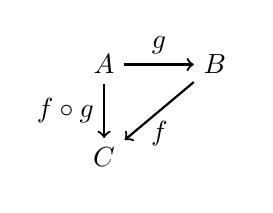
\begin{tikzpicture}[every node/.style={midway}] \matrix[column sep={4em,between origins},         row sep={2em}] at (0,0) { \node(A)   {$A$}  ; & \node(B) {$B$}; \\   \node(C) {$C$};                   \\}; \draw[<-,thick] (C) -- (A) node[anchor=east]  {$f\circ g$}; \draw[->,thick] (B) -- (C) node[anchor=north]  {$f$}; \draw[->,thick] (A)   -- (B) node[anchor=south] {$g$}; \end{tikzpicture}\end{center}


\subsection{\label{sub:Operaciones-entre-proposiciones}Operaciones entre proposiciones}

En en sistema axiomático son importantes las operaciones que se pueden
realizar con sus elementos, pero en este punto es necesario definir
lo que es una operación.

\begin{definicionn}{Operación binaria} Dados tres conjuntos $A,B$
y $C$ no vacíos, una operación binaria es una aplicación de la forma
:

\begin{center}%
\begin{tabular}{cccc}
$\otimes$: & $A\times B$ & $\rightarrow$ & %
$C$%
\tabularnewline
 & $\left(x,y\right)$ & $\mapsto$ & $z$\tabularnewline
\end{tabular}\end{center}\vspace{-5pt}\end{definicionn}

\notacion Si $\left(\left(x,y\right),z\right)\in\otimes$ se denota
$x\otimes y=z.$

Si convenimos en considerar el conjunto $U$ de todas las posibles
proposiciones del lenguaje como conjunto universo, y además el conjunto
$V=\{v,f\}$ el conjunto de los valores de verdad de una proposición.
Entonces podemos definir las siguientes aplicaciones :

\begin{center} %
\begin{tabular}{cccc}
$P$: & $U$ & $\rightarrow$ & $V$\tabularnewline
 & $p$ & $\mapsto$ & $x$\tabularnewline
\end{tabular}, %
\begin{tabular}{cccc}
$\otimes$ : & $V\times V$ & $\rightarrow$ & %
$V$%
\tabularnewline
 & $\left(x,y\right)$ & $\mapsto$ & $z$\tabularnewline
\end{tabular}, %
\begin{tabular}{cccc}
$R_{\otimes}$ : & $U\times U$ & $\rightarrow$ & %
$U$%
\tabularnewline
 & $\left(p,q\right)$ & $\mapsto$ & $r$\tabularnewline
\end{tabular}y %
\begin{tabular}{cccc}
$O_{\otimes}$ : & $U\times U$ & $\rightarrow$ & %
$V\times V$%
\tabularnewline
 & $\left(p,q\right)$ & $\mapsto$ & $(x,y)$\tabularnewline
\end{tabular}\end{center}

\begin{lista}

\item La aplicación $P$ establece que a cada proposición se le puede
asignar un valor y sólo un valor de verdad, lo que está de acuerdo
con la definición, y que cada proposición tiene asignado un valor
de verdad.

\item La operación $\otimes$ establece que dados dos valores de
verdad estos se pueden operar y obtener un único valor de verdad

\item La operación $R_{\otimes}$ establece que dadas dos proposiciones
se pueden operar y obtener una única proposición.

\item La operación $O_{\otimes}$ establece que dadas dos proposiciones
se pueden operar y obtener una pareja ordenada de valores de verdad.

\end{lista}

Teniendo en cuenta las aplicaciones definidas podemos establecer las
siguientes estructuras 

\begin{center}
\begin{large}
 \begin{tikzcd}[row sep=2cm,column sep=2cm,inner sep=1ex]
    U\times U \arrow[thick,green!40!black]{dr}[green!40!black]{\times}\arrow[thick,red]{r}[thick,red]{R_\otimes} \arrow[thick,blue]{d}[swap]{O_\otimes} & U \arrow[thick,red]{d}{P} \\
    V\times V \arrow[thick,blue]{r}[swap]{\otimes} &V \\
  \end{tikzcd}
  \end{large}
  \end{center}



\begin{center} $\times\,:\, U\times U\overset{O_{\otimes}}{\rightarrow}V\times V\overset{\otimes}{\rightarrow}V$
\end{center}

de tal forma que dadas dos proposiciones se pueden operar sus valores
de verdad bajo la operación $\times$.

Usando ésta estructura podemos definir las siguientes operaciones
entre proposiciones.

\nota En este curso no demostraremos que las operaciones están bien
definidas, es decir que es una función y el conjunto de partida es
igual al conjunto de llegada.




\subsubsection{Conjunción}

La conjunción es la operación de la forma %
\begin{tabular}{cccc}
$O_{\wedge}$ : & $U\times U$ & $\rightarrow$ & %
$U$%
\tabularnewline
 & $\left(p,q\right)$ & $\mapsto$ & $p\wedge q$\tabularnewline
\end{tabular}de tal forma que se pueden operar sus valores de verdad usando la
definición %
\begin{tabular}{cccc}
\oper{$\wedge$}\,: & $V\times V$ & $\rightarrow$ & %
$V$%
\tabularnewline
 & $\left(x,y\right)$ & $\mapsto$ & $z$\tabularnewline
\end{tabular}, obtenemos una estructura de la forma: $\wedge:\: U\times U\overset{O_{\wedge}}{\rightarrow}V\times V\overset{\oper{\ensuremath{\wedge}}\,}{\rightarrow}V$.

\begin{definicionn}{ Conjunción} La ley que establece la conjunción
es la siguiente: la conjunción es verdadera, sólo si las dos proposiciones
son verdaderas.\end{definicionn} 
\begin{table}[H]
\centering

\caption{Tabla de verdad de la conjunción}


\setlength\arrayrulewidth{1pt}\arrayrulecolor{ptctitle} 

\begin{tabular}{c|c|c}
\arrayrulecolor{ptctitle}\hline\cellcolor{ptctitle!50}$p$ & \cellcolor{ptctitle!50}$q$ & \cellcolor{ptctitle!50}$p\wedge q$\tabularnewline
\hline\cellcolor{ptcbackground}$v$ & \cellcolor{ptcbackground} $v$ & \cellcolor{ptcbackground}$v$\tabularnewline
\hline\cellcolor{gray!50}$v$ & \cellcolor{gray!50} $f$ & \cellcolor{gray!50}$f$\tabularnewline
\hline\cellcolor{ptcbackground}$f$ & \cellcolor{ptcbackground} $v$ & \cellcolor{ptcbackground}$f$\tabularnewline
\hline\cellcolor{gray!50}$f$ & \cellcolor{gray!50} $f$ & \cellcolor{gray!50}$f$\tabularnewline
\end{tabular}
\end{table}


\begin{ejem}{Conjunción}Sí $p:\:4<7$ y $q:\ 6\,\mbox{ es número par}$.
Calcular el valor de verdad de $p\wedge q.$ \end{ejem}

\solucion 
\begin{table}[H]
\centering

\caption{Tabla de verdad}


\begin{tabular}{c|c|c}
\arrayrulecolor{ptctitle}\cellcolor{gray!50}$p$ & \cellcolor{gray!50}$q$ & \cellcolor{gray!50}$p\wedge q$\tabularnewline
\hline 
\cellcolor{ptcbackground}$v$ & \cellcolor{ptcbackground}$v$ & \cellcolor{ptcbackground}$v$\tabularnewline
\hline 
\end{tabular}
\end{table}



\subsubsection{Disyunción}

La disyunción es la operación de la forma %
\begin{tabular}{cccc}
$O_{\vee}$ : & $U\times U$ & $\rightarrow$ & %
$U$%
\tabularnewline
 & $\left(p,q\right)$ & $\mapsto$ & $p\vee q$\tabularnewline
\end{tabular}de tal forma que se pueden operar sus valores de verdad usando la
definición %
\begin{tabular}{cccc}
\oper{$\vee$}\,: & $V\times V$ & $\rightarrow$ & %
$V$%
\tabularnewline
 & $\left(x,y\right)$ & $\mapsto$ & $z$\tabularnewline
\end{tabular}, obtenemos una estructura de la forma: $\vee\::\, U\times U\overset{O_{\vee}}{\rightarrow}V\times V\overset{\oper{\ensuremath{\vee}}\,}{\rightarrow}V$.

\begin{definicionn}{ Conjunción} La ley que establece la disyunción
es la siguiente: la disyunción es falsa, sólo si las dos proposiciones
son falsas.\end{definicionn} 
\begin{table}[H]
\centering

\caption{Tabla de verdad de la disyunción}


\setlength\arrayrulewidth{1pt}\arrayrulecolor{ptctitle} 

\begin{tabular}{c|c|c}
\arrayrulecolor{ptctitle}\hline\cellcolor{ptctitle!50}$p$ & \cellcolor{ptctitle!50}$q$ & \cellcolor{ptctitle!50}$p\vee q$\tabularnewline
\hline\cellcolor{ptcbackground}$v$ & \cellcolor{ptcbackground} $v$ & \cellcolor{ptcbackground}$v$\tabularnewline
\hline\cellcolor{gray!50}$v$ & \cellcolor{gray!50} $f$ & \cellcolor{gray!50}$v$\tabularnewline
\hline\cellcolor{ptcbackground}$f$ & \cellcolor{ptcbackground} $v$ & \cellcolor{ptcbackground}$v$\tabularnewline
\hline\cellcolor{gray!50}$f$ & \cellcolor{gray!50} $f$ & \cellcolor{gray!50}$f$\tabularnewline
\end{tabular}
\end{table}


\begin{ejem}{Disyunción}Sí $p:\:7>9$ y $q:\ 4<5$. Calcular el
valor de verdad de $p\vee q.$ \end{ejem}

\solucion 
\begin{table}[H]
\centering

\caption{Tabla de verdad}


\begin{tabular}{c|c|c}
\arrayrulecolor{ptctitle}\cellcolor{gray!50}$p$ & \cellcolor{gray!50}$q$ & \cellcolor{gray!50}$p\vee q$\tabularnewline
\hline 
\cellcolor{ptcbackground}$f$ & \cellcolor{ptcbackground}$v$ & \cellcolor{ptcbackground}$v$\tabularnewline
\hline 
\end{tabular}
\end{table}



\subsubsection{Condicional}

La condicional es la operación de la forma %
\begin{tabular}{cccc}
$O_{\rightarrow}$ : & $U\times U$ & $\rightarrow$ & %
$U$%
\tabularnewline
 & $\left(p,q\right)$ & $\mapsto$ & $p\rightarrow q$\tabularnewline
\end{tabular}de tal forma que se pueden operar sus valores de verdad usando la
definición %
\begin{tabular}{cccc}
\oper{$\rightarrow$}\,: & $V\times V$ & $\rightarrow$ & %
$V$%
\tabularnewline
 & $\left(x,y\right)$ & $\mapsto$ & $z$\tabularnewline
\end{tabular}, obtenemos una estructura de la forma: $\rightarrow\,:\, U\times U\overset{O_{\rightarrow}}{\rightarrow}V\times V\overset{\oper{\ensuremath{\rightarrow}}\,}{\rightarrow}V$.

\nota En la condicional a la proposición $p$ se le llama antecedente
y a $q$ consecuente.

\begin{definicionn}{ Condicional} La ley que establece la condicional
es la siguiente: la bicondicional es verdadera cuando las dos proposiciones
tienen el mismo valor de verdad.\end{definicionn}

\begin{table}[H]
\centering

\caption{Tabla de verdad de la bicondicional}


\setlength\arrayrulewidth{1pt}\arrayrulecolor{ptctitle} 

\begin{tabular}{c|c|c}
\arrayrulecolor{ptctitle}\hline\cellcolor{ptctitle!50}$p$ & \cellcolor{ptctitle!50}$q$ & \cellcolor{ptctitle!50}$p\longleftrightarrow q$\tabularnewline
\hline\cellcolor{ptcbackground}$v$ & \cellcolor{ptcbackground} $v$ & \cellcolor{ptcbackground}$v$\tabularnewline
\hline\cellcolor{gray!50}$v$ & \cellcolor{gray!50} $f$ & \cellcolor{gray!50}$f$\tabularnewline
\hline\cellcolor{ptcbackground}$f$ & \cellcolor{ptcbackground} $v$ & \cellcolor{ptcbackground}$f$\tabularnewline
\hline\cellcolor{gray!50}$f$ & \cellcolor{gray!50} $f$ & \cellcolor{gray!50}$v$\tabularnewline
\end{tabular}
\end{table}


\begin{ejem}{Condicional}Sea $p:$ Cristóbal Colón descubrió América.
; $q:\,6+3=8$ Hallar el valor de verdad de $p\rightarrow q$ \end{ejem}

\solucion 
\begin{table}[H]
\centering

\caption{Tabla de verdad}


\begin{tabular}{c|c|c}
\arrayrulecolor{ptctitle}\cellcolor{gray!50}$p$ & \cellcolor{gray!50}$q$ & \cellcolor{gray!50}$p\leftrightarrow q$\tabularnewline
\hline 
\cellcolor{ptcbackground}$v$ & \cellcolor{ptcbackground}$f$ & \cellcolor{ptcbackground}$f$\tabularnewline
\hline 
\end{tabular}
\end{table}



\subsubsection{Bicondicional}

La bicondicional es la operación de la forma %
\begin{tabular}{cccc}
$O_{\longleftrightarrow}$ : & $U\times U$ & $\rightarrow$ & %
$U$%
\tabularnewline
 & $\left(p,q\right)$ & $\mapsto$ & $p\leftrightarrow q$\tabularnewline
\end{tabular}de tal forma que se pueden operar sus valores de verdad usando la
definición %
\begin{tabular}{cccc}
\oper{$\leftrightarrow$}\,: & $V\times V$ & $\rightarrow$ & %
$V$%
\tabularnewline
 & $\left(x,y\right)$ & $\mapsto$ & $z$\tabularnewline
\end{tabular}, obtenemos una estructura de la forma: $\leftrightarrow\,:\, U\times U\overset{O_{\leftrightarrow}}{\rightarrow}V\times V\overset{\oper{\ensuremath{\leftrightarrow}}\,}{\rightarrow}V$.

\begin{definicionn}{ Bicondicional} La ley que establece la bicondicional
es la siguiente: la bicondicional es verdadera cuando las dos proposiciones
tienen el mismo valor de verdad.\end{definicionn}

\begin{table}[H]
\centering

\caption{Tabla de verdad de la bicondicional}


\setlength\arrayrulewidth{1pt}\arrayrulecolor{ptctitle} 

\begin{tabular}{c|c|c}
\arrayrulecolor{ptctitle}\hline\cellcolor{ptctitle!50}$p$ & \cellcolor{ptctitle!50}$q$ & \cellcolor{ptctitle!50}$p\longleftrightarrow q$\tabularnewline
\hline\cellcolor{ptcbackground}$v$ & \cellcolor{ptcbackground} $v$ & \cellcolor{ptcbackground}$v$\tabularnewline
\hline\cellcolor{gray!50}$v$ & \cellcolor{gray!50} $f$ & \cellcolor{gray!50}$f$\tabularnewline
\hline\cellcolor{ptcbackground}$f$ & \cellcolor{ptcbackground} $v$ & \cellcolor{ptcbackground}$f$\tabularnewline
\hline\cellcolor{gray!50}$f$ & \cellcolor{gray!50} $f$ & \cellcolor{gray!50}$v$\tabularnewline
\end{tabular}
\end{table}


\begin{ejem}{Bicondicional}Sea $p:$ Cristóbal Colón descubrió América.
; $q:\,6+3=8$ Hallar el valor de verdad de $p\rightarrow q$ \end{ejem}

\solucion

\begin{table}[H]
\centering

\caption{Tabla de verdad}


\begin{tabular}{c|c|c}
\arrayrulecolor{ptctitle}\cellcolor{gray!50}$p$ & \cellcolor{gray!50}$q$ & \cellcolor{gray!50}$p\rightarrow q$\tabularnewline
\hline 
\cellcolor{ptcbackground}$v$ & \cellcolor{ptcbackground}$f$ & \cellcolor{ptcbackground}$f$\tabularnewline
\hline 
\end{tabular}
\end{table}



\subsubsection{Disyunción exclusiva}

La disyunción exclusiva es la operación de la forma %
\begin{tabular}{cccc}
$O_{\veebar}$ : & $U\times U$ & $\rightarrow$ & %
$U$%
\tabularnewline
 & $\left(p,q\right)$ & $\mapsto$ & $p\veebar q$\tabularnewline
\end{tabular}de tal forma que se pueden operar sus valores de verdad usando la
definición %
\begin{tabular}{cccc}
\oper{$\veebar$}\,: & $V\times V$ & $\rightarrow$ & %
$V$%
\tabularnewline
 & $\left(x,y\right)$ & $\mapsto$ & $z$\tabularnewline
\end{tabular}, obtenemos una estructura de la forma: $\veebar\,:\, U\times U\overset{O_{\veebar}}{\rightarrow}V\times V\overset{\oper{\ensuremath{\veebar}}\,}{\rightarrow}V$.

\begin{definicionn}{ Disyunción exclusiva} La ley que establece
la disyunción exclusiva es la siguiente: la disyunción exclusiva es
falsa cuando las dos proposiciones tienen el mismo valor de verdad.\end{definicionn}

\begin{table}[H]
\centering

\caption{Tabla de verdad de la bicondicional}


\setlength\arrayrulewidth{1pt}\arrayrulecolor{ptctitle} 

\begin{tabular}{c|c|c}
\arrayrulecolor{ptctitle}\hline\cellcolor{ptctitle!50}$p$ & \cellcolor{ptctitle!50}$q$ & \cellcolor{ptctitle!50}$p\veebar q$\tabularnewline
\hline\cellcolor{ptcbackground}$v$ & \cellcolor{ptcbackground} $v$ & \cellcolor{ptcbackground}$f$\tabularnewline
\hline\cellcolor{gray!50}$v$ & \cellcolor{gray!50} $f$ & \cellcolor{gray!50}$v$\tabularnewline
\hline\cellcolor{ptcbackground}$f$ & \cellcolor{ptcbackground} $v$ & \cellcolor{ptcbackground}$v$\tabularnewline
\hline\cellcolor{gray!50}$f$ & \cellcolor{gray!50} $f$ & \cellcolor{gray!50}$f$\tabularnewline
\end{tabular}
\end{table}


\begin{ejem}{Disyunción exclusiva}Sea $p:$ Cristóbal Colón descubrió
América. ; $q:\,6+3=8$ Hallar el valor de verdad de $p\veebar q$
\end{ejem}

\nota Ésta operación se llama excluyente porque porque sólo se puede
dar ambas pero no una sola. 

\solucion

\begin{table}[H]
\centering

\caption{Tabla de verdad}


\begin{tabular}{c|c|c}
\arrayrulecolor{ptctitle}\cellcolor{gray!50}$p$ & \cellcolor{gray!50}$q$ & \cellcolor{gray!50}$p\veebar q$\tabularnewline
\hline 
\cellcolor{ptcbackground}$v$ & \cellcolor{ptcbackground}$f$ & \cellcolor{ptcbackground}$v$\tabularnewline
\hline 
\end{tabular}
\end{table}



\subsubsection{Negación}

La negación es la operación de la forma %
\begin{tabular}{cccc}
$O_{\sim}$ : & $U$ & $\rightarrow$ & %
$U$%
\tabularnewline
 & $p$ & $\mapsto$ & $q$\tabularnewline
\end{tabular}de tal forma que se pueden operar su valor de verdad usando la definición
\begin{tabular}{cccc}
$\sim$ : & $V$ & $\rightarrow$ & %
$V$%
\tabularnewline
 & $x$ & $\mapsto$ & $z$\tabularnewline
\end{tabular}.

\begin{definicionn}{Negación} La ley que establece la negación es
la siguiente: La negación cambia el valor de verdad de una proposición.\end{definicionn}

\begin{table}[H]
\centering

\caption{Tabla de verdad de la negación.}


\begin{tabular}{c|c}
\arrayrulecolor{ptctitle}\cellcolor{ptctitle!50}$p$ & \cellcolor{ptctitle!50}$\sim p$\tabularnewline
\hline 
\cellcolor{ptcbackground}$v$ & \cellcolor{ptcbackground}$f$\tabularnewline
\hline 
\cellcolor{gray!50}$f$ & \cellcolor{gray!50} $v$\tabularnewline
\end{tabular}
\end{table}



\subsection{\label{sub:Relaciones-entre-proposiciones}Relaciones entre proposiciones}

En esta sección trabajaremos con tautologías y falacias por lo que
presentaremos algunos ejemplos para aprender a determinar cuando una
proposición es una tautología, contingencia ó falacia.

\begin{ejems}{Tautológias}
\begin{enumerate}
\item $p\vee\sim p$ (principio del tercio excluido) 
\item $\left[(p\rightarrow q)\wedge p\right]\rightarrow q$
\item $\sim\left(p\wedge\sim p\right)$
\end{enumerate}
\end{ejems}

\solucion
\begin{enumerate}
\item Vemos que en la última columna de la tabla de verdad (\ref{tau1})
nos muestra que $p\vee\sim p$ es una tautología. 
\begin{table}[H]
\centering

\caption{Tabla de verdad.}
\label{tau1}

\begin{tabular}{c|c|c}
\arrayrulecolor{ptctitle}\cellcolor{ptctitle!50}$p$ & \cellcolor{ptctitle!50}$\sim p$ & \cellcolor{ptctitle!50}$p\vee\sim p$\tabularnewline
\hline 
\cellcolor{ptcbackground} $v$ & \cellcolor{ptcbackground}$f$ & \cellcolor{ptcbackground}$v$\tabularnewline
\hline 
\cellcolor{gray!50}$f$ & \cellcolor{gray!50} $v$ & \cellcolor{gray!50}$v$\tabularnewline
\hline 
\end{tabular}
\end{table}

\item Si observamos en la tabla de verdad (\ref{tau2}) nos queda demostrado
que $\left[(p\rightarrow q)\wedge p\right]\rightarrow q$ es una tautología.
\begin{table}[H]
\centering

\caption{Tabla de verdad.}
\label{tau2}

\begin{tabular}{c|c|c|c|c}
\arrayrulecolor{ptctitle}\cellcolor{ptctitle!50}$p$ & \cellcolor{ptctitle!50}$q$ & \cellcolor{ptctitle!50}$p\rightarrow q$ & \cellcolor{ptctitle!50}$\left(p\rightarrow q\right)\wedge p$ & \cellcolor{ptctitle!50}$\left[\left(p\rightarrow p\right)\wedge p\right]\rightarrow q$\tabularnewline
\hline 
\cellcolor{ptcbackground} $v$ & \cellcolor{ptcbackground}$v$ & \cellcolor{ptcbackground}$v$ & \cellcolor{ptcbackground}$v$ & \cellcolor{ptcbackground}$v$\tabularnewline
\hline 
\cellcolor{gray!50}$v$ & \cellcolor{gray!50} $f$ & \cellcolor{gray!50}$f$ & \cellcolor{gray!50}$f$ & \cellcolor{gray!50}$v$\tabularnewline
\hline 
\cellcolor{ptcbackground}$f$ & \cellcolor{ptcbackground} $v$ & \cellcolor{ptcbackground} $v$ & \cellcolor{ptcbackground}$f$ & \cellcolor{ptcbackground}$v$\tabularnewline
\hline 
\cellcolor{gray!50} $f$ & \cellcolor{gray!50} $f$ & \cellcolor{gray!50} $v$ & \cellcolor{gray!50}$f$ & \cellcolor{gray!50}$v$\tabularnewline
\hline 
\end{tabular}
\end{table}

\item Este queda de ejercicio al lector.
\end{enumerate}
\begin{ejems}{Falacias}
\begin{enumerate}
\item $p\wedge\sim p$ (principio de contradicción) 
\item $(p\rightarrow q)\wedge\left(p\wedge\sim q\right)$
\item $\sim\left(p\vee\sim p\right)$
\end{enumerate}
\end{ejems}

\solucion
\begin{enumerate}
\item Vemos que en la última columna de la tabla de verdad (\ref{fal1})
nos muestra que $p\wedge\sim p$ es una falacia. 
\begin{table}[H]
\centering

\caption{Tabla de verdad.}
\label{fal1}

\begin{tabular}{c|c|c}
\arrayrulecolor{ptctitle}\cellcolor{ptctitle!50}$p$ & \cellcolor{ptctitle!50}$\sim p$ & \cellcolor{ptctitle!50}$p\wedge\sim p$\tabularnewline
\hline 
\cellcolor{ptcbackground} $v$ & \cellcolor{ptcbackground}$f$ & \cellcolor{ptcbackground}$f$\tabularnewline
\hline 
\cellcolor{gray!50}$f$ & \cellcolor{gray!50} $v$ & \cellcolor{gray!50}$f$\tabularnewline
\hline 
\end{tabular}
\end{table}

\item Si observamos en la tabla de verdad (\ref{fal2}) nos queda demostrado
que $(p\rightarrow q)\wedge\left(p\wedge\sim q\right)$ es una falacia.
\begin{table}[H]
\centering

\caption{Tabla de verdad.}
\label{fal2}

\begin{tabular}{c|c|c|c|c}
\arrayrulecolor{ptctitle}\cellcolor{ptctitle!50}$p$ & \cellcolor{ptctitle!50}$q$ & \cellcolor{ptctitle!50}$p\rightarrow q$ & \cellcolor{ptctitle!50}$p\wedge\sim q$ & \cellcolor{ptctitle!50}$(p\rightarrow q)\wedge\left(p\wedge\sim q\right)$\tabularnewline
\hline 
\cellcolor{ptcbackground} $v$ & \cellcolor{ptcbackground}$v$ & \cellcolor{ptcbackground}$v$ & \cellcolor{ptcbackground}$f$ & \cellcolor{ptcbackground}$f$\tabularnewline
\hline 
\cellcolor{gray!50}$v$ & \cellcolor{gray!50} $f$ & \cellcolor{gray!50}$f$ & \cellcolor{gray!50}$v$ & \cellcolor{gray!50}$f$\tabularnewline
\hline 
\cellcolor{ptcbackground}$f$ & \cellcolor{ptcbackground} $v$ & \cellcolor{ptcbackground} $v$ & \cellcolor{ptcbackground}$f$ & \cellcolor{ptcbackground}$f$\tabularnewline
\hline 
\cellcolor{gray!50} $f$ & \cellcolor{gray!50} $f$ & \cellcolor{gray!50} $v$ & \cellcolor{gray!50}$f$ & \cellcolor{gray!50}$f$\tabularnewline
\hline 
\end{tabular}
\end{table}

\item Este queda de ejercicio al lector
\end{enumerate}

\subsubsection{Implicación}

\begin{definicionn}{Implicación} Se dice que una proposición $q$
se deduce de $p$ o que una proposición $p$ implica una proposición
$q$ cuando $p\rightarrow q$ es una tautología.\end{definicionn}

\notacion  Si una proposición $p$ implica a una proposición $q$
se denota $p\Rightarrow q.$

\begin{ejem}{Implicación}

Determinar si $\left[\left(\sim p\vee q\right)\wedge\sim q\right]\Rightarrow\sim p$
\end{ejem}

\solucion 
\begin{table}[H]
\centering

\caption{Tabla de verdad.}


\begin{tabular}{c|c|c|c|c|c|c}
\arrayrulecolor{ptctitle}\cellcolor{ptctitle!50}$p$ & \cellcolor{ptctitle!50}$q$ & \cellcolor{ptctitle!50}$\sim p$ & \cellcolor{ptctitle!50}$\sim p\vee q$ & \cellcolor{ptctitle!50}$\sim q$ & \cellcolor{ptctitle!50}\foreignlanguage{english}{$\left(\sim p\vee q\right)\wedge\sim q$} & \cellcolor{ptctitle!50}$\left[\left(\sim p\vee q\right)\wedge\sim q\right]\rightarrow\sim p$ \tabularnewline
\hline 
\cellcolor{ptcbackground} $v$ & \cellcolor{ptcbackground}$v$ & \cellcolor{ptcbackground}$f$ & \cellcolor{ptcbackground}$f$ & \cellcolor{ptcbackground}$v$ & \cellcolor{ptcbackground}$v$ & \cellcolor{ptcbackground}$v$\tabularnewline
\hline 
\cellcolor{gray!50}$v$ & \cellcolor{gray!50} $f$ & \cellcolor{gray!50}$f$ & \cellcolor{gray!50}$f$ & \cellcolor{gray!50}$v$ & \cellcolor{gray!50}$f$ & \cellcolor{gray!50}$v$\tabularnewline
\hline 
\cellcolor{ptcbackground}$f$ & \cellcolor{ptcbackground} $v$ & \cellcolor{ptcbackground} $v$ & \cellcolor{ptcbackground}$f$ & \cellcolor{ptcbackground}$v$ & \cellcolor{ptcbackground}$v$ & \cellcolor{ptcbackground}$v$\tabularnewline
\hline 
\cellcolor{gray!50} $f$ & \cellcolor{gray!50} $f$ & \cellcolor{gray!50} $v$ & \cellcolor{gray!50}$f$ & \cellcolor{gray!50}$v$ & \cellcolor{gray!50}$v$ & \cellcolor{gray!50}$v$\tabularnewline
\hline 
\end{tabular}
\end{table}


\begin{ejem}{Implicación}

Determinar si $\left(p\wedge\sim p\right)\Rightarrow q$ \end{ejem}

\solucion 
\begin{table}[H]
\centering

\caption{Tabla de verdad.}


\begin{tabular}{c|c|c|c|c}
\arrayrulecolor{ptctitle}\cellcolor{ptctitle!50}$p$ & \cellcolor{ptctitle!50}$q$ & \cellcolor{ptctitle!50}$\sim p$ & \cellcolor{ptctitle!50}$p\wedge\sim p$ & \cellcolor{ptctitle!50}$\left(p\wedge\sim p\right)\rightarrow q$\tabularnewline
\hline 
\cellcolor{ptcbackground} $v$ & \cellcolor{ptcbackground}$v$ & \cellcolor{ptcbackground}$f$ & \cellcolor{ptcbackground}$f$ & \cellcolor{ptcbackground}$v$\tabularnewline
\hline 
\cellcolor{gray!50}$v$ & \cellcolor{gray!50} $f$ & \cellcolor{gray!50}$f$ & \cellcolor{gray!50}$f$ & \cellcolor{gray!50}$v$\tabularnewline
\hline 
\cellcolor{ptcbackground}$f$ & \cellcolor{ptcbackground} $v$ & \cellcolor{ptcbackground} $v$ & \cellcolor{ptcbackground}$f$ & \cellcolor{ptcbackground}$v$\tabularnewline
\hline 
\cellcolor{gray!50} $f$ & \cellcolor{gray!50} $f$ & \cellcolor{gray!50} $v$ & \cellcolor{gray!50}$f$ & \cellcolor{gray!50}$v$\tabularnewline
\hline 
\end{tabular}
\end{table}



\subsubsection{Equivalencia lógica}

\begin{definicionn}{Equivalencia lógica} Se dice que una proposición
$q$ es equivalente a $p$, cuando $p\leftrightarrow q$ es una tautología.\end{definicionn}

\notacion  Si una proposición $p$ es equivalente a una proposición
$q$ se denota $p\Leftrightarrow q$ ó $p\equiv q.$

\begin{ejem}{Equivalencia lógica}Analice el valor de verdad de la
proposición compuesta \ensuremath{(p\rightarrow q)\leftrightarrow(\sim q\rightarrow\sim p)}
\end{ejem}

\solucion

%
\begin{tabular}{ccccccc} \ensuremath{p} &  \ensuremath{q} &  \ensuremath{p\rightarrow q} &  \ensuremath{\sim q} &  \ensuremath{\sim p} &  \ensuremath{\sim q\rightarrow\sim p} &  \ensuremath{(p\rightarrow q)\leftrightarrow(\sim q\rightarrow\sim p)}\\V  &  V  &  V  &  F  &  F  &  V  &  V\\V  &  F  &  F  &  V  &  F  &  F  &  V\\F  &  V  &  V  &  F  &  V  &  V  &  V\\F  &  F  &  V  &  V  &  V  &  V  &  V \end{tabular}\ 

%
Es decir las proposiciones: $p\rightarrow q$ y $\sim q\rightarrow\sim p$\ son
equivalentes.

\begin{ejem}{Equivalencia lógica}

Probar usando las tablas de verdad que las proposiciones $(p\rightarrow q)$
y $(\sim q\rightarrow\sim p)$, son lógicamente equivalentes. 

\end{ejem}

\solucion Para probar que las proposiciones $(p\rightarrow q)$ y
$(\sim q\rightarrow\sim p)$ son lógicamente equivalentes debemos
probar que $(p\rightarrow q)$ $\leftrightarrow$ $(\sim q\rightarrow\sim p)$
es una tautología. 
\begin{table}[H]
\centering

\caption{Tabla de verdad.}
\label{equil1}

\begin{tabular}{c|c|c|c|c|c|c}
\arrayrulecolor{ptctitle}\cellcolor{ptctitle!50}$p$ & \cellcolor{ptctitle!50}$q$ & \cellcolor{ptctitle!50}$\sim p$ & \cellcolor{ptctitle!50}$\sim q$ & \cellcolor{ptctitle!50}$p\rightarrow q$ & \cellcolor{ptctitle!50}\foreignlanguage{english}{$\sim q\rightarrow\sim p$} & \cellcolor{ptctitle!50}$(p\rightarrow q)$ $\leftrightarrow$ $(\sim q\rightarrow\sim p)$\tabularnewline
\hline 
\cellcolor{ptcbackground} $v$ & \cellcolor{ptcbackground}$v$ & \cellcolor{ptcbackground}$f$ & \cellcolor{ptcbackground}$f$ & \cellcolor{ptcbackground}$v$ & \cellcolor{ptcbackground}$v$ & \cellcolor{ptcbackground}$v$\tabularnewline
\hline 
\cellcolor{gray!50}$v$ & \cellcolor{gray!50} $f$ & \cellcolor{gray!50}$f$ & \cellcolor{gray!50}$v$ & \cellcolor{gray!50}$f$ & \cellcolor{gray!50}$f$ & \cellcolor{gray!50}$v$\tabularnewline
\hline 
\cellcolor{ptcbackground}$f$ & \cellcolor{ptcbackground} $v$ & \cellcolor{ptcbackground} $v$ & \cellcolor{ptcbackground}$f$ & \cellcolor{ptcbackground}$v$ & \cellcolor{ptcbackground}$v$ & \cellcolor{ptcbackground}$v$\tabularnewline
\hline 
\cellcolor{gray!50} $f$ & \cellcolor{gray!50} $f$ & \cellcolor{gray!50} $v$ & \cellcolor{gray!50}$v$ & \cellcolor{gray!50}$v$ & \cellcolor{gray!50}$v$ & \cellcolor{gray!50}$v$\tabularnewline
\hline 
\end{tabular}
\end{table}


\nota Para verificar si dos proposiciones son lógicamente equivalentes
basta comprobar que las dos proposiciones tienen la misma tabla de
verdad. Como se observa en la tabla (\ref{equil1}) al comparar las
columnas $5$ y $6$.


\subsection{Cuantificadores y otras formas de expresar la implicación}

En algunos casos las condicionales, vienen expresadas de tal forma
que cada proposición simple se puede representar como un conjunto,
por ejemplo 
\begin{equation}
\mbox{Los polígonos de cuatro lados son cuadriláteros.}\label{ec1}
\end{equation}
 En este caso llamaremos $P_{x}=\{x:x\ \mbox{es un polígono}\}$\ y
$Q_{x}=\{x:x\ \mbox{es un cuadrilátero}\}$ %
\footnote{A las proposiciones que dependen de una variable y de un conjunto
referencia, como es el caso de $P_{x}$\
y $Q_{x}$ se llaman proposiciones abiertas. %
} y representamos la proposición (\ref{ec1}) como $P_{x}\rightarrow Q_{x}$,
pero a nosotros nos interesan son las implicaciones, por tanto veamos
cuando está proposición es verdadera. Para ello tomaremos otro conjunto
$U_{x}=\{x:x\ \mbox{es una figura plana}\}$, a este conjunto lo llamaremos
universal o de referencia. Ahora realizaremos un diagrama de Venn
mostrado en la figura(\ref{impli})

\begin{figure}[H]
\definecolor{qqqqff}{rgb}{0,0,1}
\definecolor{ffttww}{rgb}{1,0.2,0.4}
\definecolor{ttttff}{rgb}{0.2,0.2,1}
\definecolor{zzttqq}{rgb}{0.6,0.2,0} 
\definecolor{cqcqcq}{rgb}{0.75,0.75,0.75}
\centering
\begin{tikzpicture}[line cap=round,font=\fontsize{6}{6}\selectfont,line join=round,>=triangle 45,x=1.0cm,y=1.0cm]
\clip(1,0.42) rectangle (9.53,3.71);
\fill[color=zzttqq,fill=zzttqq,fill opacity=0.1] (1.5,3.5) -- (1.5,1) -- (5,1) -- (5,3.5) -- cycle; \fill[color=zzttqq,fill=zzttqq,fill opacity=0.1] (5.5,3.5) -- (5.5,1) -- (9,1) -- (9,3.5) -- cycle;
\draw [color=zzttqq] (1.5,3.5)-- (1.5,1);
\draw [color=zzttqq] (1.5,1)-- (5,1);
\draw [color=zzttqq] (5,1)-- (5,3.5);
\draw [color=zzttqq] (5,3.5)-- (1.5,3.5);
\draw [color=zzttqq] (5.5,3.5)-- (5.5,1);
\draw [color=zzttqq] (5.5,1)-- (9,1);
\draw [color=zzttqq] (9,1)-- (9,3.5);
\draw [color=zzttqq] (9,3.5)-- (5.5,3.5);
\draw [rotate around={-20.14:(3.26,2.23)},line width=2pt,color=ttttff,fill=ttttff,fill opacity=0.1] (3.26,2.23) ellipse (1.58cm and 0.87cm);
\draw [rotate around={-17.08:(7.14,2.21)},line width=2pt,color=ttttff,fill=ttttff,fill opacity=0.1] (7.14,2.21) ellipse (1.48cm and 0.88cm);
\draw [line width=2pt,color=ffttww,fill=ffttww,fill opacity=0.1] (3.22,2.23) circle (0.64cm);
\draw [line width=2pt,color=ffttww,fill=ffttww,fill opacity=0.1] (7.27,2.07) circle (0.63cm); \draw (4.00,3.41) node[anchor=north west] {$\mathbf{U_x}$};
\draw (2.07,3.07) node[anchor=north west] {$\mathbf{P_x}$};
\draw (3.12,2.79) node[anchor=north west] {$\mathbf{Q_x}$};
\draw (4.0,2.26) node[anchor=north west] {$\mathbf{x_1}$}; 
\draw (5.99,2.94) node[anchor=north west] {$\mathbf{P_x}$};
\draw (7.63,3.47) node[anchor=north west] {$\mathbf{U_x}$};
\draw (7.18,2.11) node[anchor=north west] {$\mathbf{x_2}$};
\draw (6.96,2.64) node[anchor=north west] {$\mathbf{Q_x}$};
\draw (2.81,0.84) node[anchor=north west] {Diagrama 1};
\draw (6.76,0.83) node[anchor=north west] {Diagrama 2};
\fill [color=qqqqff] (7.22,1.86) circle (1.5pt);
\fill [color=qqqqff] (4.16,1.86) circle (1.5pt);
\end{tikzpicture}\caption{Proposiciones abiertas}\label{impli}
\end{figure}


Si tomamos un polígono, el cual representaremos con el símbolo $x_{1}$,\
observamos en el diagrama 1 que $x_{2}$\ no está en el conjunto
de los cuadriláteros, por tanto en este caso $P_{x}\rightarrow Q_{x}$\ es
falsa, mientras en el diagrama 2 tomaremos un polígono representado
por $x_{2}$\ el cual está en $Q_{x}$,\ por tanto $P_{x}\rightarrow Q_{x}$\ es
verdadera, de lo que podemos concluir que para que $P_{x}\rightarrow Q_{x}$\ sea
una tautología debe cumplirse la relación. 
\[
Q_{x}\subseteq P_{x}
\]
 Para indicar que $P_{x}\rightarrow Q_{x}$\ es una tautología utilizamos
unos operadores lógicos de existencia, los cuales son: \begin{lista} 

\item Existe algún: Se representa $\exists x$\ y se lee existe
algún $x.$ 

\item Para todo: se representa $\forall x$\ y se lee para todo
$x.$ 

\item Existe un único: Se representa $\exists\,!x$\ y se lee existe
uno y sólo un $x.$ 

\item Ningún: Se representa $\sim\exists x$\ y se lee no existe
ningún $x.$ \end{lista} En nuestro caso la proposición quedaría:
\[
\forall x\in U,\,(p_{x}\Longrightarrow q_{x})
\]
 De aquí en adelante el conjunto que representa a la proposición se
representará con letras mayúsculas y las proposiciones con letras
minúsculas con la variable como subíndice: 

Analicemos nuevamente el diagrama 2 de la figura (\ref{impli}) Como,
$x_{2}$\ está en el conjunto, entonces podemos decir que $P$ es
condición suficiente para que $x_{2}$\ esté en el conjunto $Q$.
En este sentido, se dice que $p_{x}$ es condición suficiente para
$q_{x}$. Además es claro que para que un elemento $x_{2}$ esté en
$P$\ se necesita que $x_{2}$ esté en en $Q$. De aquí que se diga
que $q_{x}$ es condición necesaria para $p_{x}.$ También se observa
que un elemento $x_{2}$ está en el conjunto $Q$ si está en el conjunto
$P$. Este análisis precedente sugiere otras maneras de expresar la
implicación 
\[
p_{x}\Longrightarrow q_{x}
\]
 éstas son:
\begin{enumerate}
\item $p_{x}$ implica a $q_{x}$
\item $p_{x}$ es condición suficiente para $q_{x}$
\item $q_{x}$ es condición necesaria para $p_{x}$
\item $q_{x},$ si $p_{x}$ 
\end{enumerate}

\subsubsection{Negación de los cuantificadores}

La regla general para construir la negación de una proposición abierta
es la siguiente: Los $\forall$ se cambian por o $\exists$ y los
$\exists$ se cambian por \foreignlanguage{english}{$\forall$} y
después se niega la proposición abierta. 

La negación de la proposición se construye mecánicamente del mismo
modo como se o a realiza la negación de una proposición . 


\section{Inferencia y esquemas de razonamiento}


\subsection{Principales leyes lógicas o tautológicas}

Siguiendo las construcción axiomática de la lógica nos queda establecer
los axiomas y los teoremas, cual estableceremos en ésta sección. 

\begin{ideas}{Leyes de inferencia lógica}

Dadas dos proposiciones $p$ y $q$ al término $p\equiv q$ se le
llama ley de inferencia.

\end{ideas}

En la lógica los teoremas son leyes de inferencia.


\subsubsection{Axiomas}

Estableceremos tres axiomas,

\begin{axioma}{ Toda proposición es idéntica a si misma, es decir
$p\equiv p$}{Identidad}\end{axioma}

\begin{axioma}{ una proposición no puede ser cierta y falsa a la
vez, es decir $\sim\left(p\wedge\sim p\right)\equiv v.$}{Contradicción}\end{axioma}

\begin{axioma}{ Toda proposición es cierta ó es falsa , es decir
$p\vee\sim p\equiv v.$}{Tercer excluido}\end{axioma}


\subsubsection{Leyes de inferencia}

\begin{ley}{Involutiva}

$\sim\left(\sim p\right)\equiv p$

\end{ley}

\begin{ley}{Indempotencia}
\begin{enumerate}
\item $p\wedge p\equiv p$
\item $p\vee p\equiv p$
\end{enumerate}
\end{ley}

\begin{ley}{Comutativas}
\begin{enumerate}
\item $\left(p\wedge q\right)\equiv\left(q\wedge p\right)$
\item $\left(p\vee q\right)\equiv\left(q\vee p\right)$
\item $p\leftrightarrow q\equiv q\leftrightarrow p$
\end{enumerate}
\end{ley}

\begin{ley}{Asociativas}
\begin{enumerate}
\item $p\wedge\left(q\wedge r\right)\equiv\left(p\wedge q\right)\wedge r$
\item $p\vee\left(q\vee r\right)\equiv\left(p\vee q\right)\vee r$
\item $p\leftrightarrow\left(q\leftrightarrow r\right)\equiv\left(p\leftrightarrow q\right)\leftrightarrow r$
\end{enumerate}
\end{ley}

\begin{ley}{Distributivas}
\begin{enumerate}
\item $p\wedge\left(q\vee r\right)\equiv\left(p\wedge q\right)\vee\left(p\wedge r\right)$
\item $p\vee\left(q\wedge r\right)\equiv\left(p\vee q\right)\wedge\left(p\vee r\right)$
\item $p\rightarrow\left(q\vee r\right)\equiv\left(p\rightarrow q\right)\vee\left(p\rightarrow r\right)$
\item $p\rightarrow\left(q\wedge r\right)\equiv\left(p\rightarrow q\right)\wedge\left(p\rightarrow r\right)$
\end{enumerate}
\end{ley}

\begin{ley}{Morgan}
\begin{enumerate}
\item $\sim\left(p\wedge q\right)\equiv\sim p\vee\sim q$
\item $\sim\left(p\vee q\right)\equiv\sim p\wedge\sim q$
\end{enumerate}
\end{ley}

\begin{ley}{Del condicional}
\begin{enumerate}
\item $p\rightarrow q\equiv\sim p\vee q$
\item $\sim\left(p\rightarrow q\right)\equiv p\wedge\sim q$
\end{enumerate}
\end{ley}

\begin{ley}{Del bicondicional}
\begin{enumerate}
\item $p\leftrightarrow q\equiv\left(p\rightarrow q\right)\wedge\left(q\rightarrow p\right)$
\item $p\leftrightarrow q\equiv\left(p\wedge q\right)\vee\left(\sim p\vee\sim q\right)$
\end{enumerate}
\end{ley}

\begin{ley}{De la absorción}
\begin{enumerate}
\item $p\wedge\left(p\text{\ensuremath{\vee}\ensuremath{q}}\right)\equiv p$
\item $p\wedge\left(\sim p\vee q\right)\equiv p\wedge q$
\item $p\vee\left(p\wedge q\right)\equiv p$
\item $p\vee\left(\sim p\wedge q\right)\equiv p\vee q$
\end{enumerate}
\end{ley}

\begin{ley}{De transposición}
\begin{enumerate}
\item $\left(p\rightarrow q\right)\equiv\sim q\rightarrow\sim p$ contrareciproco
\item $p\leftrightarrow q\equiv\sim q\leftrightarrow\sim p$
\end{enumerate}
\end{ley}

\begin{ley}{De exportación}
\begin{enumerate}
\item $\left(p\wedge q\right)\rightarrow r\equiv p\rightarrow\left(q\rightarrow r\right)$
\item $\left(p_{1}\wedge p_{2}\wedge p_{3}\wedge\cdots\wedge p_{n}\right)\rightarrow r\equiv\left(p_{1}\wedge p_{2}\wedge p_{3}\wedge\cdots\wedge p_{n-1}\right)\rightarrow\left(p_{n}\rightarrow r\right)$
\end{enumerate}
\end{ley}

\begin{ley}{De los modulos}
\begin{enumerate}
\item $p\wedge v\equiv p$ 
\item $p\vee f\equiv p$
\end{enumerate}
\end{ley}

\begin{ley}{De la simplificación}
\begin{enumerate}
\item $\left(p\vee q\right)\wedge\left(p\vee\sim q\right)\equiv p$
\item $\left(p\wedge q\right)\vee\left(p\wedge\sim q\right)\equiv p$
\end{enumerate}
\end{ley}

\nota Estas Leyes son muy útiles para simplificar los problemas,
puesto que es válido reemplazar una proposición por su equivalente
sin alterar el resultado. 

\begin{ejems}{}

Simplificar las proposiciones siguientes aplicando las leyes lógicas 
\begin{enumerate}
\item $\left[\left(p\vee\sim q\right)\wedge q\right]\rightarrow p$
\item $\sim\left[\sim\left(p\wedge q\right)\rightarrow\sim q\right]\vee q$
\item $\left[\left(\sim p\wedge q\right)\rightarrow\left(r\wedge\sim r\right)\right]\wedge\sim q$
\end{enumerate}
\end{ejems}

\solucion
\begin{enumerate}
\item Apliquemos las leyes de inferencia 
\begin{eqnarray*}
\left[\left(p\vee\sim q\right)\wedge q\right]\rightarrow p & \equiv & \sim\left[\left(p\vee\sim q\right)\wedge q\right]\vee p\\
 & \equiv & \left[\sim\left(p\vee\sim q\right)\vee\sim q\right]\vee p\\
 & \equiv & \left[\sim\left(p\vee\sim q\right)\right]\vee\left(p\vee\sim q\right)\\
 & \equiv & \left(\sim\left(p\vee\sim q\right)\vee p\right)\vee\sim q\\
 & \equiv & \left(\left[\sim p\wedge\sim q\right]\vee p\right)\vee\sim q\\
 & \equiv & \left[\left(\sim p\vee p\right)\wedge\left(\sim q\vee p\right)\right]\vee\sim q\\
 & \equiv & \left[v\wedge\left(\sim q\vee p\right)\right]\vee\sim q\\
 & \equiv & \left(\sim q\vee p\right)\vee\sim q\\
 & \equiv & \left(p\vee\sim q\right)\vee\sim q\\
 & \equiv & p\vee\left(\sim q\vee\sim q\right)\\
 & \equiv & p\vee\sim q
\end{eqnarray*}

\item Apliquemos las leyes de inferencia
\begin{eqnarray*}
\sim\left[\sim\left(p\wedge q\right)\rightarrow\sim q\right]\vee q & \equiv & \left[\sim\left(p\wedge q\right)\wedge\sim\left(\sim q\right)\right]\vee q\\
 & \equiv & \left[\left(\sim p\vee\sim q\right)\wedge q\right]\vee q\\
 & \equiv & \left[\left(\sim p\wedge q\right)\vee\left(\sim q\wedge q\right)\right]\vee q\\
 & \equiv & \left[\left(\sim p\wedge\sim q\right)\vee f\right]\vee q\\
 & \equiv & \left(\sim p\wedge\sim q\right)\vee q\\
 & \equiv & \left(\left(\sim p\vee q\right)\wedge\left(\sim q\vee q\right)\right)\\
 & \equiv & \left(\sim p\vee q\right)\wedge v\\
 & \equiv & \sim p\vee q
\end{eqnarray*}

\item Queda de tarea al lector.
\end{enumerate}

\subsection{\label{sub:Esquemas-de-razonamiento}Esquemas de razonamiento}


\subsubsection{Método inductivo}

El razonamiento inductivo es el proceso mediante el cual se obtienen
conclusiones a partir de nuestras propias observaciones o a partir
de ejemplos particulares, es decir al observar que una acción o propiedad
se repite se concluye en general que esa acción o propiedad siempre
es cierta 

\begin{ideas}{Conjetura}

Es la conclusión que se obtiene a partir de un proceso inductivo 

\end{ideas}

\nota Al utilizar el razonamiento inductivo debemos tener cuidado
de no construir conjeturas o generalizaciones falsas, por lo siempre
hay que tratar de encontrar casos donde no se cumpla la conjetura,
en caso de que no se consiga, no quiere decir que la conjetura es
cierta, sólo nos indica que no hemos encontrado un caso donde no se
cumple. A continuación mostraremos un ejemplo para explicar paso a
paso como podemos obtener una conjetura a partir de una secuencia
de casos o fenómenos. Aunque en ese ejemplo no trataremos de verificar
si la conjetura es siempre cierta, el objetivo es de aprender a construir
conjeturas. 

\begin{ejem}{} Suponga que una persona mide los lados de cuatro triángulos
como muestra la figura(\ref{dest}). Establezca una conjetura sobre
los lados de un triángulo

\end{ejem}

\begin{figure}[H]


\centering\caption{Desigualdad triangular}
\label{dest}

 \definecolor{xdxdff}{rgb}{0.49,0.49,1}
\definecolor{qqqqff}{rgb}{0,0,1}
\begin{tikzpicture}[scale=2.0, font=\fontsize{8}{9}\selectfont,line cap=round,line join=round,>=triangle 45,x=1.0cm,y=1.0cm] 
\clip(-2.49,3.16) rectangle (4.47,5.53);
\draw (-1.92,3.96)-- (-1.15,3.96); 
\draw (-1.92,3.96)-- (-1.38,4.5); 
\draw (-1.38,4.5)-- (-1.15,3.96);
\draw (0.2,4.68)-- (-0.07,3.97);
\draw (0.2,4.68)-- (0.51,3.98); 
\draw (0.51,3.98)-- (-0.07,3.97);
\draw (1.42,4.22)-- (2.03,4.22);
\draw (1.07,4.72)-- (1.42,4.22); 
\draw (1.07,4.72)-- (2.03,4.22); 
\draw (3.44,4.72)-- (3.02,4.27);
\draw (3.44,4.72)-- (3.89,4.3); 
\draw (3.89,4.3)-- (3.02,4.27);
\begin{scriptsize} 
\fill [color=qqqqff] (-1.92,3.96) circle (1.5pt);
\draw[color=qqqqff] (-2.04,3.97) node {$A$};
\fill [color=xdxdff] (-1.15,3.96) circle (1.5pt);
\draw[color=xdxdff] (-1.06,3.88) node {$B$};
\draw[color=black] (-1.56,3.84) node {$0.77$};
\fill [color=xdxdff] (-1.38,4.5) circle (1.5pt);
\draw[color=xdxdff] (-1.4,4.75) node {$C$}; 
\draw[color=black] (-1.88,4.43) node {$0.77$};
\draw[color=black] (-0.96,4.29) node {$0.59$};
\fill [color=qqqqff] (0.2,4.68) circle (1.5pt);
\draw[color=qqqqff] (0.19,4.85) node {$D$}; \fill [color=xdxdff] (-0.07,3.97) circle (1.5pt); \draw[color=xdxdff] (-0.22,3.97) node {$E$};
\draw[color=black] (-0.2,4.51) node {$0.76$};
\fill [color=xdxdff] (0.51,3.98) circle (1.5pt);
\draw[color=xdxdff] (0.67,4) node {$F$};
\draw[color=black] (0.58,4.4) node {$0.75$};
\draw[color=black] (0.26,3.84) node {$0.58$};
\fill [color=qqqqff] (1.42,4.22) circle (1.5pt);
\draw[color=qqqqff] (1.39,4.03) node {$G$};
\fill [color=xdxdff] (2.03,4.22) circle (1.5pt);
\draw[color=xdxdff] (2.14,4.39) node {$H$};
\draw[color=black] (1.71,4.11) node {$0.61$}; 
\fill [color=xdxdff] (1.07,4.72) circle (1.5pt);
\draw[color=xdxdff] (1.14,4.89) node {$I$};
\draw[color=black] (1.12,4.32) node {$0.61$};
\draw[color=black] (1.66,4.68) node {$1.08$};
\fill [color=xdxdff] (3.02,4.27) circle (1.5pt);
\draw[color=xdxdff] (2.9,4.29) node {$K$}; 
\draw[color=black] (2.99,4.64) node {$0.62$};
\fill [color=qqqqff] (3.44,4.72) circle (1.5pt);
\draw[color=qqqqff] (3.43,4.91) node {$J$};
\fill [color=xdxdff] (3.89,4.3) circle (1.5pt);
\draw[color=xdxdff] (4.11,4.31) node {$L$};
\draw[color=black] (3.46,4.16) node {$0.62$};
\draw[color=black] (3.84,4.64) node {$0.88$};
\end{scriptsize}
\end{tikzpicture}

\end{figure}


De acuerdo con la figura \ref{dest} tenemos que en $\triangulo ABC $ se tiene: \begin{eqnarray} 
AC+AB & = & 1.54 > BC = 0.31 \\
AB + BC & = & 1.36> AC =  0.77 \end{eqnarray}
En el $\triangulo DEF$ se tiene que  
\begin{eqnarray}
DE+DF & = & 1.51 > EF=0.58 \\
DE + EF &=& 1.48> AC =0.75 \end{eqnarray}
En el $\triangulo IGH$ se tiene que 
\begin{eqnarray} IG+GH & = & 1.22 > HI=1.08 \\
IG + IH &=& 1.69> GH=0.61 \end{eqnarray} 
En el $\triangulo JKL$ se tiene que 
\begin{eqnarray}
JK+KL & = & 1.29 > JL=0.88 \\
JK + JL &=& 1.50> KL=0.75 
\end{eqnarray}

De los anteriores resultados , a pesar que los triángulos $ABC$,
$HIG$ y $JKL$ son isósceles, podemos concluir. \textquotedbl{} Que
la suma de las longitudes de dos lados de un triángulo siempre es
menor que la longitud de su tercer lado\textquotedbl{}


\subsubsection{Método del contraejemplo}

Hay ocasiones donde después de un razonamiento inductivo obtenemos
una conjetura que no se cumple para todos los casos, es decir obtenemos
una generalización falsa, entonces para indicar que esa generalización
es falsa buscamos un ejemplo donde no se cumpla la acción o la propiedad. 

\begin{ideas}{Contraejemplo}Es el método que se usa para demostrar
que una generalización es falsa, utilizando un ejemplo que la contradiga.
\end{ideas}

\nota\ Los ejemplos sólo son validos para demostrar que una proposición
es falsa, nunca demuestra que una proposición es verdadera. \begin{ejem}{Contraejemplo}Si
un cuadrilátero tiene sus diagonales perpendiculares, entonces es
un rombo.\end{ejem}

\begin{figure}[H]
\centering

\caption{Cometa}
\label{com}\definecolor{qqwuqq}{rgb}{0.13,0.13,0.13}
\definecolor{uququq}{rgb}{0.25,0.25,0.25}
\definecolor{xdxdff}{rgb}{0.66,0.66,0.66}
\definecolor{qqqqff}{rgb}{0.33,0.33,0.33}
\begin{tikzpicture}[scale=1.2,line cap=round,line join=round,>=triangle 45,x=1.0cm,y=1.0cm]
\clip(-3.42,-1.42) rectangle (2.68,5.54);
\draw[color=qqwuqq,fill=qqwuqq,fill opacity=0.1] (0.59,2.02) -- (0.58,2.44) -- (0.16,2.44) -- (0.16,2.01) -- cycle; 
\draw (0.12,4.92)-- (0.2,-0.54);
\draw (0.12,4.92)-- (2.1,2.04);
\draw (2.1,2.04)-- (0.2,-0.54);
\draw (0.12,4.92)-- (-2.96,1.97);
\draw (-2.96,1.97)-- (0.2,-0.54);
\draw (-2.96,1.97)-- (2.1,2.04);
\begin{scriptsize}
\fill [color=qqqqff] (0.12,4.92) circle (1.5pt);
\draw[color=qqqqff] (0.12,5.24) node {$A$};
\fill [color=qqqqff] (0.2,-0.54) circle (1.5pt);
\draw[color=qqqqff] (0.22,-0.74) node {$B$};
\fill [color=qqqqff] (2.1,2.04) circle (1.5pt);
\draw[color=qqqqff] (2.26,2.3) node {$C$}; 
\draw[color=black] (1.66,3.54) node {$3.49$}; 
\fill [color=xdxdff] (-2.96,1.97) circle (1.5pt);
\draw[color=xdxdff] (-3.08,2.22) node {$D$};
\draw[color=black] (-1.9,3.58) node {$4.27$};
\fill [color=uququq] (0.16,2.01) circle (1.5pt);
\draw[color=uququq] (-0.1,1.84) node {$E$};
\draw[color=qqwuqq] (0.46,2.72) node {$90\degre$};
\end{scriptsize} 
\end{tikzpicture}

\end{figure}


En el cuadrilátero podemos observar que $AD=6.29$ y $AC=6$ y por
definición de rombo el cuadrilátero $ABCD$ no puede ser un rombo
porque no tiene sus lados congruentes.


\subsubsection{Razonamiento deductivo}

El método deductivo consiste en partir de un número reducido de información
(hipótesis) y mediante un proceso lógico deducir otros conocimientos
o proposiciones nuevas. Para profundizar y entender este método explicaremos
a continuación cuales son los procesos lógicos. 


\subsubsection{Prueba indirecta (Tollendo-tollens)}

Es un razonamiento de la forma: 

\begin{center}
\begin{tabular}{c}
$p\longrightarrow q$\tabularnewline
$\sim q$ \tabularnewline
\hline\tabularnewline
$\sim p$ \tabularnewline
\end{tabular}
\par\end{center}

\begin{ejem}{}
\[
\begin{tabular}[t]{rl}
 \ensuremath{p\rightarrow q:} &  Si dos rectas son paralelas, entonces no tienen puntos en común.\medskip\\
\ensuremath{\sim q:} &  Las rectas \ensuremath{\overleftrightarrow{l_{1}}}y \ensuremath{\overleftrightarrow{l_{2}}}tienen un punto en común.\medskip\medskip\\
\hline \medskip\\
\ensuremath{\sim p:} &  Las rectas \ensuremath{\overleftrightarrow{l_{1}}}y \ensuremath{\overleftrightarrow{l_{2}}}no son paralelas. 
\end{tabular}\ 
\]
 \vspace{-10pt}\end{ejem}

Como la condicional debe ser una implicación, entonces tenemos que
para que ella sea una tautología, solo existen dos posibilidades,
que las dos proposiciones $p$ y $q$ tengan el mismo valor de verdad.
Por tanto si $q$ es falsa se deduce que $p$ también es falsa.\foreignlanguage{english}{ }


\subsubsection{Modus ponendus ponens (Directa)}

Este es un razonamiento de la forma: 

\begin{center}
\begin{tabular}{c}
$p\longrightarrow q$\tabularnewline
$p$ \tabularnewline
\hline\tabularnewline
$p$ \tabularnewline
\end{tabular}
\par\end{center}

La argumentación es la misma de la prueba indirectas decir para que
$p\longleftrightarrow q$ sea una implicación si $p$ es verdadera,
se tiene que $q$ también lo es. 

\begin{ejem}{}

%
\[
\begin{tabular}[t]{rl}
 \ensuremath{p\rightarrow q:} &  Si un triángulo tiene tres ángulos congruentes, entonces es equilátero.\medskip\\
\ensuremath{p:} &  El triángulo \ensuremath{\triangle ABC}tiene tres ángulos congruentes\medskip\\
\hline \\
\ensuremath{q:} &  El triangulo \ensuremath{\triangle ABC}es equilátero. 
\end{tabular}\ \ 
\]


%
\end{ejem}


\subsubsection{Regla de la cadena}

Este razonamiento es el más usado en matemáticas consiste en construir
una cadena de implicaciones partiendo de la hipótesis hasta obtener
la conclusión y es de la forma: 

\begin{center}
\begin{tabular}{c}
$p\longrightarrow r$\tabularnewline
$r\longrightarrow q$\tabularnewline
\hline\tabularnewline
$p\longrightarrow q$.\tabularnewline
\end{tabular}
\par\end{center}

\begin{ejem}{}
\[
\begin{tabular}{lll}
 \ensuremath{p\rightarrow q:} &  \ensuremath{\text{Si dos rectas son perpendiculares, entonces se intersecan.}}\medskip\  &  \\
\ensuremath{q\rightarrow r:} &  \ensuremath{\text{Si dos rectas se intersecan, entonces no son paralelas.}}\medskip\  &  \\
\hline \\
\ensuremath{p\rightarrow r:} &  \ensuremath{\text{Si dos rectas son perpendiculares, entonces no son paralelas.}} &  
\end{tabular}\ \ 
\]
 \end{ejem} Otra forma de interpretar este razonamiento es: 
\[
\left(p\longrightarrow r\wedge r\longrightarrow q\right)\longrightarrow\left(p\longrightarrow q\right),
\]
 mirándola de esta forma el razonamiento es equivalente si la conjunción
es cierta entonces la conclusión también lo es decir $p\longrightarrow q$
es una tautología. 

\begin{ejem}{}Sea $\overleftrightarrow{ED}$ una mediatriz del segmento
$\overline{AB}$ en el $\triangulo{ABC}$, si el punto $F$ es la
intersección de lado $AB$ y la mediatriz, entonces $\overline{AF}\cong\overline{FB}.$
\end{ejem}

\begin{figure}[H]


\centering\caption{Regla de la cadena}
\label{Pmedio}

\definecolor{xdxdff}{rgb}{0.49,0.49,1} \definecolor{uququq}{rgb}{0.25,0.25,0.25} \definecolor{qqqqff}{rgb}{0,0,1} \begin{tikzpicture}[scale=0.9,font=\fontsize{9}{8}\selectfont,line cap=round,line join=round,>=triangle 45,x=1.0cm,y=1.0cm,line width=1.2pt] \clip(-0.59,-1.42) rectangle (4.72,2.48); \draw (0.37,-0.25)-- (3.55,-0.27); \draw[<->] (1.96,-1.42) -- (1.96,2.48); \draw (0.37,-0.25)-- (3.08,1.35); \draw (3.08,1.35)-- (3.55,-0.27); \fill [color=qqqqff] (0.37,-0.25) circle (1.5pt); \draw[color=qqqqff] (0.22,-0.19) node {$A$}; \fill [color=qqqqff] (3.55,-0.27) circle (1.5pt); \draw[color=qqqqff] (3.71,-0.17) node {$B$}; \fill [color=qqqqff] (3.08,1.35) circle (1.5pt); \draw[color=qqqqff] (3.18,1.51) node {$C$}; \draw[color=black] (2.12,3.96) node {$b$}; \draw[color=black] (1.86,0.47) node {$c$}; \draw[color=black] (3.16,0.58) node {$d$}; \fill [color=uququq] (1.96,-0.26) circle (1.5pt); \draw[color=uququq] (2.11,-0.38) node {$F$}; \fill [color=xdxdff] (1.97,1.91) circle (1.5pt); \draw[color=xdxdff] (2.07,2.07) node {$E$}; \fill [color=xdxdff] (1.96,-1.14) circle (1.5pt); \draw[color=xdxdff] (2.06,-0.97) node {$D$}; \end{tikzpicture}

\end{figure}


\solucion Para demostrar que ésta proposición es una implicación
vamos a utilizar el método de razonamiento deductivo, de la si\-gui\-ente
manera:

\begin{figure}[H]
\centering

\caption{Solución}
\label{solej}

\definecolor{zzttqq}{rgb}{0.6,0.2,0} \definecolor{cqcqcq}{rgb}{0.75,0.75,0.75} \begin{tikzpicture}[scale=2.0,font=\fontsize{6}{6}\selectfont,line cap=round,line join=round,>=triangle 45,x=1.0cm,y=1.0cm,line width=1.2pt] \clip(-1.11,-1.66) rectangle (5.96,2.71); \fill[color=zzttqq,fill=zzttqq,fill opacity=0.1] (-1,2) -- (-1,1) -- (1,1) -- (1,2) -- cycle; \fill[color=zzttqq,fill=zzttqq,fill opacity=0.1] (3,2) -- (3,1) -- (5.3,1) -- (5.31,2) -- cycle; \fill[color=zzttqq,fill=zzttqq,fill opacity=0.1] (3,0) -- (5.39,0.01) -- (5.39,-1.02) -- (3,-1) -- cycle; \draw [color=zzttqq] (-1,2)-- (-1,1); \draw [color=zzttqq] (-1,1)-- (1,1); \draw [color=zzttqq] (1,1)-- (1,2); \draw [color=zzttqq] (1,2)-- (-1,2); \draw [color=zzttqq,->] (1,1)-- (3,0); \draw (-0.95,1.65) node[anchor=north west] {$\overline{ED}$ es mediatriz de $\overline{AB}$}; \draw [->] (1,1.48) -- (2.99,1.5); \draw [color=zzttqq] (3,2)-- (3,1); \draw [color=zzttqq] (3,1)-- (5.3,1); \draw [color=zzttqq] (5.3,1)-- (5.31,2.01); \draw [color=zzttqq] (5.31,2.01)-- (3,2); \draw (3.05,1.61) node[anchor=north west] {$F$ es el punto medio de $\overline{AB}$}; \draw [->] (4.21,1) -- (4.22,0.03); \draw [color=zzttqq] (3,0)-- (5.39,0.01); \draw [color=zzttqq] (5.39,-1.02)-- (3,-1); \draw (3.9,-0.4) node[anchor=north west] {$\overline{AF}\cong \overline{FB}$}; \draw (-0.15,2.33) node[anchor=north west] {Dato}; \draw (3.3,2.3) node[anchor=north west] {Definición de mediatrz}; \draw (3.26,-1.15) node[anchor=north west] {Definición de punto medio}; \end{tikzpicture}

\end{figure}


La estructura para redactar una demostración que usaremos es la sigui\-ente. 

\begin{center}\begin{prueba}{\protect$\overline{ED}$\ es la mediatriz de \protect$\overline{AB}$}{2.& \protect$F$\ es punto medio de \protect$\overline{AB}$ & Definici\'on de punto mediatriz\\ 3. & \protect$AF\cong FB$ & Definici\'on de punto medio\\ } \end{prueba}\end{center}

Es decir en este ejemplo usamos la regla de la cadena.


\subsubsection{Ley modus tollendo-ponens }

Este razonamiento es de la forma: 

\begin{center}
\begin{tabular}{c}
$p\vee q$\tabularnewline
$\sim p$\tabularnewline
\hline\tabularnewline
$q$.\tabularnewline
\end{tabular}
\par\end{center}


\subsubsection{Ley del silogismo disyuntivo}

Es un razonamiento con la siguiente estructura 

\begin{center}
\begin{tabular}{c}
$p\vee q$\tabularnewline
$p\longrightarrow r$\tabularnewline
$q\longrightarrow s$\tabularnewline
\hline\tabularnewline
$r\vee s$.\tabularnewline
\end{tabular}
\par\end{center}

\nota\ Existen tres reglas básicas de validez que se aplican continuamente
en una demostración.\\
 Regla 1: las definiciones, los postulados y los teoremas demostrados
pueden aparecer en cualquier paso de la demostración.\\
 Regla 2: las proposiciones equivalentes se pueden sustituir entre
sí en cualquier parte de una demostración.\\
 Regla 3: una proposición verdadera se puede introducir en cualquier
punto de la demostración.

\vspace{20pt}
 \nota\ Antes de terminar la sección mostraremos, en la figura \ref{demos},
como es el esquema que se debe emplear en una demostración sin importar
como la redactemos. 

\begin{figure}[H]
\centering\caption{Esquema de una demostración}
\label{demos}

\definecolor{zzccff}{rgb}{0.6,0.8,1}
\definecolor{cqcqcq}{rgb}{0.75,0.75,0.75}
\begin{tikzpicture}[scale=1.1,line cap=round,font=\fontsize{7}{7}\selectfont,line join=round,>=triangle 45,x=1.0cm,y=1.0cm] %
%\draw [color=cqcqcq,dash pattern=on 1pt off 1pt, xstep=2.0cm,ystep=2.0cm] %(-0.27,1.66) %grid (12.29,5.02);
\clip(-0.27,1.66) rectangle (12.29,5.02); \fill[color=zzccff,fill=zzccff,fill opacity=0.1] (0,4) -- (4,4) -- (4,2) -- (0,2) -- cycle; \fill[color=zzccff,fill=zzccff,fill opacity=0.1] (4.5,3.5) -- (6.5,3.5) -- (6.5,4) -- (7.5,3) -- (6.5,2) -- (6.5,2.5) -- (4.5,2.5) -- cycle; \fill[color=zzccff,fill=zzccff,fill opacity=0.1] (8,4) -- (12,4) -- (12,2) -- (8,2) -- cycle; \draw [color=zzccff] (0,4)-- (4,4); \draw [color=zzccff] (4,4)-- (4,2); \draw [color=zzccff] (4,2)-- (0,2); \draw [color=zzccff] (0,2)-- (0,4); \draw [color=zzccff] (4.5,3.5)-- (6.5,3.5); \draw [color=zzccff] (6.5,3.5)-- (6.5,4); \draw [color=zzccff] (6.5,4)-- (7.5,3); \draw [color=zzccff] (7.5,3)-- (6.5,2); \draw [color=zzccff] (6.5,2)-- (6.5,2.5); \draw [color=zzccff] (6.5,2.5)-- (4.5,2.5); \draw [color=zzccff] (4.5,2.5)-- (4.5,3.5); \draw [color=zzccff] (8,4)-- (12,4); \draw [color=zzccff] (12,4)-- (12,2); \draw [color=zzccff] (12,2)-- (8,2); \draw [color=zzccff] (8,2)-- (8,4); \draw (0.61,3.69) node[anchor=north west] {\parbox{3.78 cm}{Términos no definidos \\ Definiciones  \\  Postulados \\  Otros  teoremas}}; \draw (1.16,4.54) node[anchor=north west] {Hipótesis}; \draw (4.48,4.52) node[anchor=north west] {Razonamieto lógico}; \draw (9.47,4.57) node[anchor=north west] {Tesis}; \draw (9.31,3.09) node[anchor=north west] {Conclusión}; \draw (4.7,3.36) node[anchor=north west] {\parbox{2.71 cm}{Esquema de  \\  razonamiento}}; \end{tikzpicture}

\end{figure}


\label{sec:problema} \problemas{ 
\begin{enumerate}
\item En los incisos del \textbf{a)} al \textbf{e)}, escriba las proposiciones
como implicaciones, luego decida si es falso o verdadero 

\begin{enumerate}
\item \textbf{Hipótesis} $p:$ Un hombre vive en Barranquilla, \textbf{Conclusión}
$q:$ Vive en Antioquía. 
\item \textbf{Hipótesis} $p:$ Algunas manzanas son rojas, \textbf{Conclusión}
$q:$ Los caballos tienen cuatro patas. 
\item \textbf{Hipótesis} $p:$ Dos rectas se intersecan, \textbf{Conclusión}
$q:$ Las dos rectas no son paralelas. 
\item \textbf{Conclusión} $q:$ Dos rectas son perpendiculares, \textbf{Hipótesis}
$p:$ Las rectas se intersecan. 
\item \textbf{Hipótesis} $p:$ Dos ángulos tienen la misma medida, \textbf{Conclusión}
$q:$ Los ángulos son congruentes. 
\end{enumerate}
\item \textbf{Analice la siguiente conjetura}: Si un triángulo tiene un
ángulo recto, tiene dos lados congruentes.\textbf{ Comentario:} Para
demostrar que la conjetura es falsa, debe presentar un contraejemplo,
para explicar que es verdadera use las definiciones. 
\item Demuestre la siguiente conjetura: Si dos ángulos son congruentes sus
complementos son congruentes. 
\item En los incisos del a) al e) identifique la hipótesis y la conclusión
y determine si es una implicación. 

\begin{enumerate}
\item un número es par si termina en 4. 
\item Dos rectas son perpendiculares si forman un ángulo recto. 
\item Un triángulo con dos lados congruentes, tiene los tres ángulos congruentes, 
\item Si Un número es impar, termina en cinco. 
\item Una recta que biseca un segmento contiene su punto medio. 
\end{enumerate}
\item Formule la recíproca, contraria y contra-reciproca , de las siguientes
proposiciones. 

\begin{enumerate}
\item Si una persona camina se acalora. 
\item Si dos rectas se intersecan, son paralelas. 
\item Si una persona es adinerada, entonces puede viajar. 
\item si $a=0$ y $b=0$, entonces $a.b=0$, para todo $a$ y $b$ reales. 
\item Si un polinomio es un triángulo, entonces una región plana. 
\item Dos planos paralelos si intersecan. 
\end{enumerate}
\item Determine en cada inciso si la proposición representa una equivalencia,
en caso de no ser lo encuentre un contra ejemplo. 

\begin{enumerate}
\item Un triángulo tiene sus lados congruentes si y sólo si tiene sus ángulos
interiores congruentes. 
\item Un ángulo es recto si y sólo si es congruente a uno que tiene medida
igual a $90\degre$. 
\item Dos rectas son paralelas si y solo si no se intersecan. 
\item Un cuadrilátero tiene sus lados opuestos paralelos, si y sólo si un
par de lados opuestos son congruentes. 
\item Dos ángulos son complementarios si y sólo si la suma de sus mediadas
es igual a $90\degre$ 
\end{enumerate}
\item Incluya la información omitida para formular un esquema de razonamiento
correcto, además indique que tipo de prueba se esta realizando. 

\begin{enumerate}
\item \scalebox{0.9}{%
\begin{tabular}{rl}
$p\Longrightarrow q:$  & Dos rectas perpendiculares se intersecan.\medskip{}
\tabularnewline
$q\Longrightarrow r:$  & Las rectas no son paralelas \medskip{}
\tabularnewline
 & ni se intersecan. \medskip{}
\tabularnewline
\hline 
\medskip{}
 & \tabularnewline
 & \tabularnewline
\end{tabular}}
\item \scalebox{0.9}{%
\begin{tabular}{rl}
$p\Longrightarrow q:$  & Si dos rectas son paralelas no \medskip{}
\tabularnewline
 & se intersecan.\medskip{}
\tabularnewline
$\sim q:$  & Las rectas no se intersecan. \medskip{}
\tabularnewline
\hline 
\medskip{}
 & \tabularnewline
 & \tabularnewline
\end{tabular}}
\item \scalebox{0.9}{%
\begin{tabular}{rl}
$p\Longrightarrow q:$  & Si un punto está en la mediatriz de un \medskip{}
\tabularnewline
 & segmento, entonces equidista de sus\medskip{}
\tabularnewline
 & extremos.\medskip{}
\tabularnewline
 & El punto no está en la mediatriz. \medskip{}
\tabularnewline
\hline 
\medskip{}
 & \tabularnewline
 & \tabularnewline
\end{tabular}}
\item \scalebox{0.9}{%
\begin{tabular}{rl}
 & \medskip{}
\tabularnewline
$p:$  & $\angle ABC$ mide más de $90\degre$ \medskip{}
\tabularnewline
\hline 
\medskip{}
 & \tabularnewline
 & El $\angle ABC$ es un ángulo obtuso \tabularnewline
\end{tabular}}
\item \scalebox{0.9}{%
\begin{tabular}{rl}
 & \medskip{}
\tabularnewline
$\sim q:$  & La temperatura aumenta. \medskip{}
\tabularnewline
\hline 
\medskip{}
 & \tabularnewline
 & No llovió. \tabularnewline
\end{tabular}}
\end{enumerate}
\item Probar la veracidad de la implicación 
\[
\text{Si }ab=0,\text{ entonces }a=0\text{ }\vee\text{ }b=0,
\]
 es equivalente a probar la veracidad de la implicación
\[
\text{Si }ab=0\text{ }\wedge\text{ }a\neq0,\text{ entonces }b=0.
\]

\item Determine el valor de verdad de la siguiente afirmación. Si es falsa,
dé un contraejemplo:
\[
\text{“Si }\overline{AB}\cong\overline{BC}\text{, entonces }B\text{ es el punto medio de }\overline{AC}\text{”.}
\]

\item ¿Será condición suficiente que $x^{2}=81$ par que $x=9$?
\item Dada la proposición ``Una condición necesaria para que $B$ sea el
punto medio de $\overline{AC}$ es que $B$ está entre los punto $A$
y $C$”.

\begin{enumerate}
\item Escr\'{i}bala de la forma \textit{si..., entonces...} sin alterar
su significado y obtenga su valor de verdad.
\item Escr\'{i}ba el condicional en términos de condición suficiente.
\item Haga el recíproco del condicional y determine su valor de verdad.
Si es falsa, dé un contraejemplo. 
\end{enumerate}
\item Dada la proposición ``Si $ab=0$, entonces $a=0$ o $b=0$”, escriba
su recíproca, su contraria y su contrarecíproca. Además determine
sus correspondientes valores de verdad.
\item ¿ Es posible que existan dos recta que no se intersecan y están en
planos diferentes? Si la respuesta es afirmativa, dé un ejemplo.
\item Tomando como conjunto universal el conjunto de los números reales,
determine si las proposiciones $p_{x}:$ $x^{2}-4=0$ y $q_{x}:$
$\left(x-2\right)\left(x+2\right)=0$ son equivalentes. Argumente
su respuesta.
\item Complete los siguientes esquemas de razonamiento:

\begin{enumerate}
\item \begin{flushleft}
\[
\begin{tabular}[t]{lll}
  &  \ensuremath{:} &  \mbox{Si un número entero termina en dos, }\medskip\\
 &   &  entonces\mbox{es par}.\medskip\\
 &  \ensuremath{:} &  \ensuremath{32}\mbox{ es un entero que termina en dos}.\medskip\\
\hline \medskip\\
\mbox{}  &  \ensuremath{:} &  ...... 
\end{tabular}\ 
\]

\par\end{flushleft}
\item \begin{flushleft}
\[
\begin{tabular}[t]{lll}
  &  \ensuremath{:} &  Si dos tectas son paralelas, \medskip\\
 &   &  entonces están en un\medskip\\
 &   &  mismo plano y no se intersecan.\medskip\\
 &  \ensuremath{:} &  .........\medskip\\
\hline \medskip\\
\mbox{}  &  \ensuremath{:} &  Las rectas \ensuremath{\overleftrightarrow{l_{1}}}y \ensuremath{\overleftrightarrow{l_{2}}}no son paralelas. 
\end{tabular}
\]

\par\end{flushleft}
\item \begin{flushleft}
$\begin{tabular}[t]{lll}
  &  \ensuremath{:} &  Dos rectas perpendiculares se \medskip\\
 &   &  intersecan. \medskip\\
 &  \ensuremath{:} &  Las rectas no son paralelas, si se \medskip\\
 &   &  intersecan.\medskip\\
\hline \medskip\mbox{}  &  \ensuremath{:} &  ........ 
\end{tabular}$ 
\par\end{flushleft}
\end{enumerate}
\item Demuestre que si $x$ e $y$ son enteros impares, entonces $xy$ también
es un entero impar.
\item Haga una demostración por reducción al absurdo del siguiente teorema:
Si $x^{2}$ es un entero par, entonces $x$ es par. \textit{Sugerencia:}
Utilice el ejercicio anterior.
\item Siendo $p:$ los precios son bajos y $q:$ los precios no suben, escribir
en lenguaje corriente las siguientes expresiones simbólicas : 

\begin{enumerate}
\item $\sim q$
\item $p\wedge q$
\item $p\wedge\sim q$
\item $\sim p\wedge\sim q$
\item $\sim\left(p\wedge\sim q\right)$
\end{enumerate}
\item Sean $p:$ tengo un loro y $q:$ tengo un gato, escribir en lenguaje
corriente y luego simplificar, 
\[
\sim\left(\sim p\vee\sim q\right)\wedge\sim\left(\sim p\right)
\]

\item Pruebe que: 

\begin{enumerate}
\item $\left(p\wedge q\right)\Leftrightarrow\sim\left(p\rightarrow\sim q\right)$
\item $\left[p\rightarrow\left(q\vee r\right)\right]\Leftrightarrow\left[\left(p\wedge\sim q\right)\rightarrow r\right]$
\end{enumerate}
\item Pruebe que: 

\begin{enumerate}
\item $\left[\left(a\rightarrow b\right)\wedge\left(b\rightarrow c\right)\right]\Rightarrow\left(a\rightarrow c\right)$
\item $\left(a\rightarrow b\right)\Rightarrow\left[\left(c\vee a\right)\rightarrow\left(c\vee b\right)\right]$
\end{enumerate}
\item Siendo $p$ y $q$ proposiciones cualesquiera, la proposición ,$(p\rightarrow q)\leftrightarrow[(p\vee q)\leftrightarrow q]$
, 

\begin{enumerate}
\item ¿Es siempre verdadera?
\item ¿Es verdadera si y sólo si $p$ lo es? 
\item ¿Es verdadera si y sólo si $q$ es falsa? 
\item ¿Es verdadera si y sólo si $p$ y $q$ lo son? 
\end{enumerate}
\item Pruebe, sin hacer uso de tablas de verdad, que: 

\begin{enumerate}
\item $p\wedge\sim q\rightarrow r\equiv\sim p\vee\left(q\vee r\right)$
\item $\left[\left(p\wedge q\right)\vee r\right]\wedge\sim q\equiv\left(r\wedge\sim q\right)$
\end{enumerate}
\item ¿ Cuál es la relación que existe entre las proposiciones siguientes?
\[
p\rightarrow\left[p\wedge\sim\left(q\vee r\right)\right]\mbox{ y \ensuremath{\sim p\vee\left(\sim q\wedge\sim r\right)}}
\]

\item Se define $\triangle$ como la conjunción negativa, es decir, $p\triangle q$
se lee ni $p$ ni o $q$. 

\begin{enumerate}
\item Construya la tabla de verdad de $p\triangle q$.
\item Pruebe que:

\begin{enumerate}
\item $\sim p\equiv p\triangle p$
\item $p\vee q\equiv\left(p\triangle q\right)\triangle\left(p\triangle q\right)$
\item $p\wedge q\equiv\left(p\triangle p\right)\triangle\left(q\triangle q\right)$
\item $\left(p\leftrightarrow q\right)\wedge\sim\left(p\wedge q\right)\equiv p\triangle q$
\end{enumerate}
\end{enumerate}
\item Simplifique la expresión:
\[
\left[\sim q\vee\left(\sim q\leftrightarrow p\right)\right]\rightarrow q
\]

\item Simplifique las siguientes expresiones

\begin{enumerate}
\item $\sim\left(p\vee q\right)\rightarrow\left(\sim p\wedge\sim q\right)$
\item $\left[\left(p\wedge q\right)\vee r\right]\wedge\sim p$
\item $\left[\left(p\rightarrow q\right)\rightarrow q\right]\rightarrow\left(p\vee q\right)$
\end{enumerate}
\item Sea $A={1,2,3,4}$ el conjunto universal. Determinar el valor de verdad
de cada enunciado: 

\begin{enumerate}
\item $\forall x:x+3<6$
\item $\forall x:x^{2}-10\leq8$
\item $\exists x:2x^{2}+x=15$
\item $\exists x:x^{2}>1\rightarrow x+2=0$
\end{enumerate}
\item Negar los siguientes enunciados

\begin{enumerate}
\item $\left[\exists y\in U:p\left(y\right)\right]\rightarrow\left[\forall x\in U:\left(\sim q\left(x\right)\right)\right]$
\item $\left[\exists x\in U:\left(\sim p\left(x\right)\right)\right]\vee\left[\forall x\in U:q\left(x\right)\right]$
\item $\exists x\forall y\in U$:$\left[\left(p\left(x,y\right)\rightarrow q\left(x,y\right)\right)\right]$
\end{enumerate}
\item Se sabe que: \medskip{}
Si Pedro no es alumno de la U.A. o Juan es alumno de la U.A., entonces
Juan es alumno de la U. Costa. \medskip{}
Si Pedro es alumno de la U.A. y Juan no es alumno de la U. A., entonces
Juan es alumno de la U.Costa. \medskip{}
Se desea saber en que universidad estudia Juan. 
\item Negar la siguiente expresión:
\[
\mbox{\ensuremath{\left(\forall\epsilon>0\right)\left(\exists\delta>0\right)\left(0<\left|x-x_{0}\right|<\delta\vee\left|f\left(x\right)-l\right|<\epsilon\right)}}
\]

\item A partir del álgebra proposicional, demostrar la validez del siguiente
a argumento:\medskip{}
 Si 2 es par, entonces 5 no es divisor de 9 por otra parte 11 no es
primo o 5 es divisor de 9. Además, 11 es primo. Por tanto, 2 es impar. 
\item Demuestre:

\begin{enumerate}
\item $p\veebar q\equiv\left(p\vee q\right)\wedge\sim\left(p\wedge q\right)$
\item $\sim\left[p\rightarrow\sim\left(q\veebar\sim p\right)\right]\leftrightarrow\left(p\wedge q\right)$
\end{enumerate}
\item Siendo $p:$ José es estudioso y $q:$ Juan es estudioso, escribir
en forma e simbólica:

\begin{enumerate}
\item José es estudioso y Juan no es estudioso.
\item Jos\'{é} no es estudioso y Juan es estudioso.
\item Jos\'{é} y Juan, no son estudiosos.
\item No es cierto que Juan o Jos\'{é} sean estudiosos. 
\end{enumerate}
\item En cual de sus significados est\'{á} “o”(no excluyente) en las siguientes
a proposiciones: 

\begin{enumerate}
\item a) Si ganase mucho dinero o ganara la lotería, haría un viaje.
\item El lunes ir\'{é} a la estaci\'{ó}n de trenes o al terminal de buses.
\item $x=3$ ó $x=2$
\end{enumerate}
\item Verificar, utilizando tablas de verdad, cuáles de las siguientes proposiciones
son equivalentes:

\begin{enumerate}
\item $p\veebar\sim q;$
\item $\sim p\vee q;$
\item $\left(p\vee\sim q\right)\wedge\left(\sim p\vee q\right);$
\item $\left(p\wedge q\right)\vee\left(\sim p\wedge\sim q\right);$
\end{enumerate}
\item Encuentre el valor de verdad de 
\[
\left[\sim\left(p\rightarrow q\right)\wedge\left(\sim p\wedge q\right)\right]\vee\left(r\rightarrow\sim p\right)
\]
\medskip{}
si $p:$ el número e es par, $q\equiv f$ y $r:$ los gatos tienen
5 patas
\item Construya las tablas de verdad de las siguientes proposiciones:

\begin{enumerate}
\item $\left[\left(p\rightarrow q\right)\rightarrow\left(q\rightarrow p\right)\right]\leftrightarrow\left(p\vee\sim q\right)$
\item $p\veebar\left(q\vee r\right)$
\item $\sim\left(\sim p\leftrightarrow q\right)$
\item $\sim\left(\sim q\leftrightarrow p\right)$
\item $\left(p\wedge\sim q\right)\rightarrow\left(\sim p\vee q\right)$
\item $\left[p\wedge\left(\sim q\rightarrow p\right)\right]\wedge\left[\left(p\leftrightarrow\sim q\right)\rightarrow\left(q\vee\sim p\right)\right]$
\end{enumerate}
\item Pruebe que son tautologías:

\begin{enumerate}
\item $\left[p\vee\left(p\wedge q\right)\leftrightarrow p\right]$
\item $\left(p\wedge q\right)\rightarrow\sim\left(\sim p\wedge\sim q\right)$
\item $q\rightarrow\left(p\rightarrow q\right)$
\item $\left(p\wedge q\right)\rightarrow r\leftrightarrow\left(p\rightarrow r\right)\vee\left(q\rightarrow r\right)$
\item $p\rightarrow\left[q\rightarrow\left(p\wedge q\right)\right]$
\item $\left(\left(p\rightarrow\left(q\wedge r\right)\right)\right)\leftrightarrow\left(\left(p\rightarrow q\right)\wedge\left(p\rightarrow r\right)\right)$
\item $\left[p\vee\left(p\wedge q\right)\right]\leftrightarrow p$
\end{enumerate}
\item Probar las siguientes equivalencias: 

\begin{enumerate}
\item $p\veebar\left(q\veebar r\right)\equiv\left(p\veebar q\right)\veebar r$
\item $p\wedge\left(q\veebar r\right)\equiv\left(p\wedge v\right)\veebar\left(p\wedge r\right)$
\item $p\vee q\equiv\left(p\veebar q\right)\veebar\left(p\wedge q\right)$
\item $p\wedge q\equiv p\veebar\left(p\wedge\sim q\right)$
\item $p\wedge\left(p\vee q\right)\equiv p$
\item $\sim\left(p\wedge q\right)\equiv\sim p\vee\sim q$
\item $p\wedge\left(q\vee r\right)\equiv\left(p\wedge q\right)\vee\left(p\wedge r\right)$
\end{enumerate}
\item 	 	 Averiguar si son equivalentes las proposiciones: \medskip{}
$(p\wedge q)\rightarrow r$ y $\left(p\rightarrow r\right)\wedge\left(q\rightarrow r\right)$
	
\item Encuentre el valor de verdad de: $\left[\left(p\rightarrow q\right)\vee\left(\sim p\wedge q\right)\right]\wedge\left(r\rightarrow q\right)$si

\begin{enumerate}
\item $p$ es $v$, $q$ es $v$, $r$ es $f$
\item $p,\, r$ son $f$, $q$ es $v$	
\item $p$ es $f$, $q$ es $f$ y $r$ es $f$
\item si todas son verdaderas 	
\end{enumerate}
\item Simplificar las siguientes proposiciones:

\begin{enumerate}
\item $p\wedge$$\left(q\wedge\sim p\right)$ 
\item $\left(p\wedge q\right)\vee p$
\item $\left(p\rightarrow q\right)\vee\text{\ensuremath{\sim}}p$
\item $\left(p\rightarrow q\right)\vee q$
\item $\left(p\rightarrow q\right)\wedge p$
\item $\left(p\rightarrow q\right)\rightarrow p$
\item $\left(p\rightarrow\sim q\right)\vee q$
\item $p\wedge\sim\left(q\rightarrow p\right)$
\item $\left[p\vee\left(q\leftrightarrow\sim p\right)\right]\rightarrow\sim q$
\item $\left[\text{\ensuremath{\sim\left(p\rightarrow q\right)}}\wedge\left(\sim p\wedge q\right)\right]\vee\left[r\rightarrow\left(p\vee r\right)\right]$
\item $\sim p\wedge\left(q\wedge p\right)$
\item $\left\{ p\rightarrow\left(\sim p\vee r\right)\right\} \wedge\left\{ r\rightarrow\sim p\right\} $
\item $\left\{ \sim\left(p\rightarrow q\right)\rightarrow\sim\left(q\rightarrow p\right)\right\} \wedge\left(p\vee q\right)$
\end{enumerate}
\item Derive a partir de las equivalencias básicas, las siguientes equivalencias: 

\begin{enumerate}
\item $\left(\left(p\wedge q\right)\rightarrow r\right)\equiv\left(\left(p\rightarrow r\right)\vee\left(q\rightarrow r\right)\right)$
\item $\left(\left(p\rightarrow q\right)\wedge q\right)\rightarrow\sim p\equiv q\rightarrow\sim p$
\end{enumerate}
\item Demostrar sin el uso de tablas de verdad: 

\begin{enumerate}
\item $p\vee\left(p\wedge q\right)\equiv p$
\item $p\wedge\left(p\vee q\right)\equiv p$
\item $\sim\left(p\vee q\right)\vee\left(\sim p\wedge q\right)\equiv\sim p$
\item $\sim\left(p\rightarrow\sim q\right)\leftrightarrow\left(p\wedge q\right)$
\item $\left(p\wedge\sim q\right)\rightarrow r\equiv\sim p\vee\left(q\vee r\right)$
\item $\left[\left\{ \left(p\rightarrow q\right)\wedge\left(p\rightarrow t\right)\right\} \vee\left\{ \left(r\rightarrow q\right)\wedge\left(r\rightarrow t\right)\right\} \right]\equiv\left[\left(p\wedge r\right)\rightarrow\left(q\wedge t\right)\right]$
\end{enumerate}
\item Exprese en símbolos lógicos y después niegue las siguientes oraciones: 

\begin{enumerate}
\item Todo múltiplo de 4 es número primo. 
\item Si 2 es par entonces todos los números son pares. 
\item Todo número mayor que 2 es la suma de dos números primos.
\end{enumerate}
\item Sea $A={0,1,2,3,4,5,6}$. Escribir en símbolos y averiguar el valor
de verdad de:

\begin{enumerate}
\item Hay un elemento que es mayor que todos. 
\item Existe un único elemento cuyocuadrado es 4. 
\item Para todos los elementos de $A$, sea $x$ el elemento que sumado
1 unidad, siempre es mayor que cero entonces su cuadrado es menor
que 35.
\item Para cada elemento existe otro que es menor o igual qué él 
\end{enumerate}
\item Si las proposiciones $a$ y $b$ son tales que la proposición $\sim(a\wedge b)\rightarrow(a\vee b)$
o es verdadera, determinar el valor de verdad de $(a\wedge b)\vee(a\vee b)$. 
\item Sea $A={1,2,3,4,5}$. Negar hallar el valor de verdad de los siguientes
enunciados 

\begin{enumerate}
\item $(\exists x\in A)(x+3=10)$
\item $\forall x\in A)(x+3<10)$
\item $(\exists x\in A)(x+3<5)$
\item $(\forall x\in A)(x+3\le7)$
\item $(\exists!x\in A)(x2\lyxmathsym{−}3x+2=0)$
\end{enumerate}
\item Si el conjunto universal es conjunto de los números naturales. Escribir
en símbolos las siguientes expresiones.

\begin{enumerate}
\item ) Todo número es mayor o igual que sí mismo.
\item Si el número  $x$ es menor que $y$, entonces no es mayor que 9.
\item Cualquier $x$ sumado con algún número resulta $x$.
\item El producto de $x$ con $y$ es mayor que $x$, y mayor que $y$. 
\end{enumerate}
\item ¿Cuáles de las siguientes proposiciones son verdaderas? 

\begin{enumerate}
\item Si $p\vee q\equiv F$ entonces $[\sim(\sim q\rightarrow p)\wedge\sim p]$
es una tautología. 
\item Es suficiente que $p\veebar q$ sea falsa para que $p$ y $q$ sean
equivalentes.
\item No es necesario que  $p$ sea verdadera y $q$ sea falsa para que
$[p\vee(q\wedge\sim p)]\wedge\sim q$ sea verdadero. 
\end{enumerate}
\item Demuestre las siguientes equivalencias sin uso de tablas de verdad. 

\begin{enumerate}
\item $(p\rightarrow q)\equiv{(p\wedge\sim q)\rightarrow q}$
\item $(p\leftrightarrow q)\equiv(\sim p\leftrightarrow\sim q)$
\item ${p\rightarrow(q\wedge r)}\equiv{(p\rightarrow q)\wedge(p\rightarrow r)}$
\item ${(p\wedge q)\rightarrow r}\equiv{(p\wedge\sim\lyxmathsym{∼}r)\rightarrow\sim q}$
\item ${p\rightarrow(p\wedge\sim(q\vee r))}\equiv\sim p\vee(\sim q\wedge\sim r)$
\item $[(\sim p\vee q)\vee(\sim r\wedge\sim p)]\equiv(q\vee\sim p)$
\end{enumerate}
\item Indique en cuáles de los siguientes casos $p$ es condición suficiente
para $q$; y en cuáles $p$ es condición necesaria y suficiente para
$q$.

\begin{enumerate}
\item $p:$ $A$ es múltiplo de 4, $q:\,\, A$es número par 
\item $p$: $A$ y $B$ son pares, $q$: $A+B$ es par.
\end{enumerate}
\item Si las proposiciones compuestas 

\begin{enumerate}
\item $p\leftrightarrow(\sim q\vee\sim r)$ y
\item $\sim p\vee q$ son siempre verdaderas. Demuestre que la proposición
$[\sim r\wedge(p\vee s)]\rightarrow s\vee q$ es también verdadera. 
\end{enumerate}
\item Negar las siguientes afirmaciones:

\begin{enumerate}
\item $\left(\forall x\exists y\in I\!\! R\right)(x+y=5\rightarrow y=\lyxmathsym{−}x)$
\item $\left(\forall x\forall y\in I\!\! R\right)[(x+y\mbox{ es impar})\rightarrow(x\mbox{ es impar}\vee y\mbox{ es impar})]$
\item $\left(\exists x\forall y\in I\!\! R\right)(x<y\wedge x^{2}\geq y)$
\item $\left(\exists z\forall y\forall x\in I\!\! R\right)(x<y\rightarrow x+z=y)$
\end{enumerate}
\item Averiguar el valor de verdad siendo $U=I\!\! R$. 

\begin{enumerate}
\item $\left(x\in I\!\! R\right)(x<0\rightarrow x<3)$ 
\item $\mbox{\mbox{\ensuremath{\left(\lyxmathsym{∃}x\lyxmathsym{∈}I\!\!\ R\right)}}}(x2\ge0\rightarrow x4=x3)$
\item $\left(\forall x\lyxmathsym{∈}I\!\! R,\lyxmathsym{∃}y\lyxmathsym{∈}I\!\! R\right)(x2+y2=1)$
\item $\left(\forall x\lyxmathsym{∈}I\!\! R,\forall y\lyxmathsym{∈}I\!\! R\right)(y<x\rightarrow2y<10$) 
\end{enumerate}
\item Dada la proposición, 8 no es impar divisible por 2, porque 9 no es
o múltiplo de 3.Niegue la proposición y Determine su valor de verdad
.
\item Dadas las proposiciones abiertas $p(x):x^{2}\ge x$ y $q(x):x\ge0$.
Determine el valor de verdad de las siguientes proposiciones: 

\begin{enumerate}
\item $[p(\frac{11}{2})\rightarrow q(1)]\rightarrow[p(x)\wedge q(x)]$
\item $\forall x\lyxmathsym{∈}I\!\! R:\lyxmathsym{∼}p(x)\rightarrow\lyxmathsym{∼}q(x)$ 
\end{enumerate}
\item Si la proposición $(p\wedge\lyxmathsym{∼}q)\rightarrow(\lyxmathsym{∼}r\rightarrow\lyxmathsym{∼}t)$
es falsa, determine el valor o de verdad de la proposición $(p\wedge t)\rightarrow(r\vee q)\rightarrow(u\leftrightarrow v)$.
\item Demostrar: 

\begin{enumerate}
\item Si $n$ es par y $m$ es impar, entonces $(n+m)$ es impar, $n,m\lyxmathsym{∈}I\!\! N)$. 
\item Si  $xy=0$ entonces $x=0\vee y=0$. 
\item Si $ab$ es impar, entonces $a$ es par y $b$ es impar. 
\end{enumerate}
\item Determine el valor de verdad de las siguientes proposiciones:

\begin{enumerate}
\item $\forall x\lyxmathsym{∈}I\!\! R:x2\ge x$
\item $\lyxmathsym{∃}x\lyxmathsym{∈}I\!\! R:2x=x$
\item $\forall x\lyxmathsym{∈}I\!\! R:\frac{{\displaystyle 2x\text{−}1}}{{\displaystyle 4x\text{−}2}}=12$
\item $\lyxmathsym{∃}x\lyxmathsym{∈}I\!\! R:x^{2}+2x+1\le0$
\item $\forall x\lyxmathsym{∈}I\!\! R:\lyxmathsym{−}x^{2}+4x\lyxmathsym{−}5>0$ 
\end{enumerate}
\end{enumerate}
					 

}


